\documentclass[10pt,aspectratio=1610,compress,dvipsnames]{beamer}

% \input@path lets \input{tex/foo} and \input{chapters/foo} resolve without
% explicit subdirectory paths in chapter files.
\makeatletter
\def\input@path{{tex/}{chapters/}}
\makeatother

\usetheme[
%%% option passed to the outer theme
%    progressstyle=fixedCircCnt,   % fixedCircCnt, movingCircCnt (default)
]{CodingTealArc}

% To override theme colors, uncomment and edit:
%\setbeamercolor{CodingTealArc}{fg=red!20,bg=red}
%\setbeamercolor{structure}{fg=red}
%\setbeamercolor{frametitle}{fg=blue}
%\setbeamercolor{normal text}{fg=black,bg=gray!10}

%-------------------------------------------------------
% PACKAGES
%-------------------------------------------------------

%\usepackage{helvet}
%\usepackage[T1]{fontenc}
%\usepackage[utf8]{inputenc}
%\usepackage{textcomp}
%\renewcommand{\ttdefault}{lmtt}

\usepackage{helvet}
\usepackage{fontspec}
\usepackage{unicode-math}
\setmainfont{TeX Gyre Termes}
%\setmathfont{TeX Gyre Termes Math}
\setmathfont{TeX Gyre Pagella Math}

\setsansfont[
Path = fonts/,
UprightFont = *Medium.ttf,
BoldFont    = *Bold.ttf
]{GmarketSansTTF}
\usepackage{textcomp}
\renewcommand{\ttdefault}{lmtt} %

% colored hyperlinks using theme color
\newcommand{\chref}[2]{
  \href{#1}{{\usebeamercolor[bg]{CodingTealArc} #2}}
}

\makeatletter
\def\blfootnote{\gdef\@thefnmark{}\@footnotetext}
\makeatother

\usepackage{listings}

\usepackage{tikz}
\usepackage{pgfplots, pgfplotstable}
\pgfplotsset{compat=1.18}
\usetikzlibrary{
	3d, % For 3D drawing
	angles,
	arrows,
	arrows.meta,
	backgrounds,
	bending,
	calc,
	decorations.pathmorphing,
	decorations.pathreplacing,
	decorations.markings,
	fit,
	matrix,
	patterns,
	patterns.meta,
	positioning,
	shadows,
	shapes,
	shapes.geometric,
	tikzmark,
	quotes
}
\usetikzlibrary{positioning, shapes.geometric, arrows}
\usetikzlibrary{patterns}
\usetikzlibrary{decorations.markings, arrows.meta}
\usetikzlibrary{decorations.pathmorphing}
\usetikzlibrary{bending, shadows.blur}
\usetikzlibrary{fit, calc, shapes}
\usetikzlibrary{mindmap}
\usetikzlibrary{tikzmark}

\usepackage{multicol}
\renewcommand{\lstlistingname}{Code}
\usepackage{array}
\usepackage{booktabs}
\usepackage{adjustbox}
\usepackage{kotex}

\usepackage{soul}
\usepackage{colortbl}
\usepackage{booktabs}

\usepackage{pdfrender}
%-------------------------------------------------------
% TITLE PAGE INFORMATION
%-------------------------------------------------------


\definecolor{myteal}{HTML}{008C8C}
\definecolor{mydarkteal}{HTML}{003F46}

\title[Coding Theory and Mathematics]
{
  \textbf{\Huge\color{myteal!70!black} Coding Theory and Mathematics}
}
\subtitle[Linear, Hamming, and Cyclic Codes]
{
  \text{\LARGE -- Linear, Hamming, and Cyclic Codes --}
%  \vspace{2cm}
}


\author[Ji, Yong-hyeon]
{\texorpdfstring{
		\vspace{.5cm}
		{\centering
			
\includegraphics[scale=1.5]{tikzs/jyh.pdf}
		}\\ [-.2cm]
	}{Ji, Yong-hyeon}}

\institute[PQC Hard Problem Colloquium]
{
	\vspace{-.5cm}
	\textbf{\Large PQC Hard Problem Colloquium}\\
	\vspace{-0.5cm}
	\vspace{1cm}
	\textbf{\large\it 2026 Spring}\\
	\vspace{-1cm}
}

\date{\today}

\usepackage{tcolorbox}
\tcbset{colback=white, arc=5pt}

% teal-family colors for math boxes
\definecolor{axiomcolor}{HTML}{00646A}
\definecolor{defcolor}{HTML}{007575}
\definecolor{procolor}{HTML}{00575E}
\definecolor{thmcolor}{HTML}{003F46}
\definecolor{lemcolor}{HTML}{006F73}
\definecolor{corcolor}{HTML}{00615F}
\definecolor{execolor}{HTML}{004F54}

\newcommand{\axiombox}[2][]{%
  \begin{tcolorbox}[colframe=axiomcolor, title={\color{white}\bfseries #1}]
    #2
  \end{tcolorbox}
}
\newcommand{\defbox}[2][]{%
  \begin{tcolorbox}[colframe=defcolor, title={\color{white}\bfseries #1}]
    #2
  \end{tcolorbox}
}
\newcommand{\lembox}[2][]{%
  \begin{tcolorbox}[colframe=lemcolor, title={\color{white}\bfseries #1}]
    #2
  \end{tcolorbox}
}
\newcommand{\probox}[2][]{%
  \begin{tcolorbox}[colframe=procolor, title={\color{white}\bfseries #1}]
    #2
  \end{tcolorbox}
}
\newcommand{\thmbox}[2][]{%
  \begin{tcolorbox}[colframe=thmcolor, title={\color{white}\bfseries #1}]
    #2
  \end{tcolorbox}
}
\newcommand{\corbox}[2][]{%
  \begin{tcolorbox}[colframe=corcolor, title={\color{white}\bfseries #1}]
    #2
  \end{tcolorbox}
}
\newcommand{\exebox}[2][]{%
  \begin{tcolorbox}[colframe=execolor, title={\color{white}\bfseries #1}]
    #2
  \end{tcolorbox}
}

\usepackage{listings}
%\definecolor{type}{HTML}{4EC9B0} %  A turquoise or teal.
\definecolor{atompurple}{rgb}{0.7, 0.4, 0.8}
\definecolor{keyword}{HTML}{8e4e9e}
\definecolor{myblue}{HTML}{3471d8}
\definecolor{type}{HTML}{4EC9B0}
\definecolor{golden}{HTML}{d19a66}

% Change "Listing" to another name, e.g., "Code"
\renewcommand{\lstlistingname}{Code}
\lstdefinestyle{normal}{
	frame=single, % Border
	basicstyle=\tt\small, % Code font style
	breaklines=true, % Break long lines into multiple lines automatically
	aboveskip=1.5\baselineskip, % Vertical whitespace before the listing
	tabsize=3, % How many space to a tab
}
\lstdefinestyle{shell}{
	keywordstyle={\bfseries\color{JungleGreen}},
	morekeywords={jasminc, -ec},
	%	numbers=left, % Line numbers location
	%	numbersep=6pt, % Whitespace to the right of line numbers
	%	numberstyle=\tiny\it, % Line numbers font style
	linewidth=\textwidth,  % Sets the listing width to match the text width
	frame=single, % Border
	basicstyle=\tt\scriptsize, % Code font style
	breaklines=true, % Break long lines into multiple lines automatically
	aboveskip=1.5\baselineskip, % Vertical whitespace before the listing
	tabsize=2, % How many space to a tab
}
\lstdefinestyle{c}{
	language=C,
	basicstyle=\ttfamily\small,        % Basic font style
	keywordstyle=\color{keyword}\bfseries,       % Keywords in bold blue
	keywordstyle=[2]\color{myblue}\bfseries,
	keywordstyle=[3]\color{magenta}\bfseries,
	keywordstyle=[4]\color{purple}\bfseries,
	stringstyle=\color{red!70},               % Strings in reddish color
	commentstyle=\color{green!50!black}\itshape, % Comments in italic green-black
	numberstyle=\tiny\color{gray},            % Line numbers in tiny gray font
	numbers=left,                             % Line numbers on the left
	stepnumber=1,                             % Number every line
	numbersep=8pt,                            % Space between line numbers and code
%	backgroundcolor=\color{gray!10},          % Light gray background
	frame=single,                             % Single-line frame around the code
	rulecolor=\color{gray},                   % Frame color
	tabsize=4,                                % Tab space width
	showstringspaces=false,                   % Don't show spaces in strings
	breaklines=true,                          % Line breaking enabled
	breakatwhitespace=true,                   % Break lines at whitespace
	captionpos=b,                             % Caption below the code
	escapeinside={\%*}{*)},                   % Allow LaTeX within code
	morekeywords={printf, scanf, main, size_t, uint8_t, uint16_t, uint32_t, uint64_t},
	morekeywords=[2]{randomSeed, hashArray,
	expandChallenge, expandATF_vec_copy, expandColumns, expandSeeds,
	invertingOnATF, actingOnATFS, columnsMatrix, columnsDecomposition,
	multiplicationModuloP, addmul_P32_into_64, reductionModuloP,
	reductionStrict, inversionModuloP},
	morekeywords=[3]{crypto_sign_keypair, crypto_sign},
	morekeywords=[4]{lu}
}
% Command to Include Rust Code
\newcommand{\ccode}[2][]{%
	\lstinputlisting[style=c,#1]{#2}
}

% Inline Code Highlighting
\newcommand{\cinline}[1]{%
	\lstinline[style=c]|#1|%
}
\lstdefinestyle{asm}{
	%	language=[x86masm]Assembler,
	language=C,
	basicstyle=\ttfamily\small,
	keywordstyle=\color{blue},
	commentstyle=\color{gray!50},
	stringstyle=\color{orange},
	morekeywords={.data, .align, .asciz, .text, .global, .type, .size, .extern, stp, mov, adr, ldr, add, bl, ret, ldp, and,
	movk, lsr, mul, sub, uxtw, cmp, blt, str, cbnz},
	numbers=none,
	frame=single,                             % Single-line frame around the code
	rulecolor=\color{gray},                   % Frame color
}

%\lstdefinestyle{jasmin}{
%	language=[x86masm]Assembler, % Closest to Jasmin syntax
%	basicstyle=\ttfamily\small, % Monospace font for code
%	keywordstyle=\color{blue}\bfseries, % Keywords in blue and bold
%	stringstyle=\color{orange}, % Strings in orange
%	commentstyle=\color{green!60!black}\itshape, % Comments in green
%	numbers=left, % Line numbers on the left
%	numberstyle=\tiny\color{gray}, % Line number style
%	stepnumber=1, % Show every line number
%	numbersep=5pt, % Space between numbers and code
%	frame=single, % Single frame around code
%	tabsize=4, % Tab width
%	showstringspaces=false, % Don't underline spaces in strings
%	breaklines=true, % Wrap long lines
%	captionpos=b, % Caption at the bottom
%	morekeywords={mov, add, sub, mul, xor, and, or, shl, shr, call, ret, lea}, % Add Jasmin-specific keywords
%	escapeinside={(*@}{@*)} % For embedding LaTeX inside code
%}



%
%% --------------------------------------------------------------------
%\newcommand{\dslash}{\mathbin{\mathsf{/\mkern-4mu/}}}
%\newcommand{\dslasheq}{\mathbin{\mathsf{/\mkern-4mu/\mkern-8mu=}}}
%\newcommand{\slasheq}{\mathbin{\mathsf{/\mkern-6mu=}}}

% --------------------------------------------------------------------
\definecolor{OliveGreen}{rgb}{0.33, 0.5, 0.18}
\definecolor{Blue}{rgb}{0.06, 0.2, 0.65}
\definecolor{grey}{rgb}{0.43, 0.5, 0.5}
\lstdefinestyle{jasmin}{
	mathescape=true,
	columns=fullflexible,
	keepspaces=true,
	captionpos=b,
	frame=tb,
%	xleftmargin=.1\textwidth,
%	xrightmargin=.1\textwidth,
	rangebeginprefix={(**\ begin\ },
	rangeendprefix={(**\ end\ },
	rangesuffix={\ *)},
	includerangemarker=false,
	basicstyle=\small\sffamily,
	identifierstyle={},
	keywordstyle=[1]{\color{OliveGreen}},
	keywordstyle=[2]{\color{keyword}\bfseries},
	keywordstyle=[3]{\color{Blue}},
	keywordstyle=[4]{\bfseries\color{OliveGreen}},
	keywordstyle=[5]{\color{Red}},
	keywordstyle=[6]{\color{golden}},
	keywordstyle=[7]{\bfseries\color{magenta}},
%	morekeywords=[7]{xor, aes, enc, dec},
	morekeywords=[2]{fn,for,to,downto,if,else,do,while,return,param},
	morekeywords=[3]{u256,u128,u64,u32,u16,u8,bool,int},
	morekeywords=[1]{reg,stack,inline,export},
	comment=[l][\color{grey}]{//},
	morecomment=[s][\color{grey}]{/*}{*/},
	alsoletter ={_},
	literate=
	{-}{-}{1}%
	{->}{$\rightarrow$}{1}%
	{4u64}{4u64}{1}%
	{>>}{$\gg$}{1}%
	{<<}{$\ll$}{1}%,
}[keywords,comments]
\newcommand{\jasmincode}[2][]{%
	\lstinputlisting[style=jasmin,#1]{#2}
}
\newcommand{\jasmininline}[1]{%
	\lstinline[style=jasmin]|#1|%
}

\newcommand{\dslash}{\mathbin{\mathsf{/\mkern-4mu/}}}
\newcommand{\dslasheq}{\mathbin{\mathsf{/\mkern-4mu/\mkern-8mu=}}}
\newcommand{\slasheq}{\mathbin{\mathsf{/\mkern-6mu=}}}
\newcommand{\drarrow}{\raisebox{.07em}{$\mathbin{\scriptstyle\mathsf{-\mkern-3mu>}}$}}
\newcommand{\dlarrow}{\raisebox{.07em}{$\mathbin{\scriptstyle\mathsf{<\mkern-3mu-}}$}}
\newcommand{\drrarrow}{\raisebox{.07em}{$\mathbin{\scriptstyle\mathsf{-\mkern-3mu>\mkern-3mu>}}$}}
\newcommand{\dllarrow}{\raisebox{.07em}{$\mathbin{\scriptstyle\mathsf{<\mkern-3mu<\mkern-3mu-}}$}}
\lstdefinestyle{easycrypt}{
	upquote=true,
	escapechar=\#,
	mathescape=false,
	columns=fullflexible,
	keepspaces=true,
	captionpos=b,
	frame=tb,
%	xleftmargin=.1\textwidth,
%	xrightmargin=.1\textwidth,
	rangebeginprefix={(**\ begin\ },
	rangeendprefix={(**\ end\ },
	rangesuffix={\ *)},
	includerangemarker=false,
	basicstyle=\small\ttfamily,
	identifierstyle={},
	keywordstyle=[1]{\bfseries\color{violet}},
	keywordstyle=[2]{\bfseries\color{olive}},
	keywordstyle=[3]{\bfseries\color{blue}},
	keywordstyle=[4]{\bfseries\color{blue}},
	keywordstyle=[5]{\bfseries\color{red}},
	keywordstyle=[6]{\bfseries\color{violet}},
	morekeywords=[1]{arg},
	morecomment=[n][\itshape]{(*}{*)},
	morecomment=[n][\bfseries]{(**}{*)},
	morekeywords=[1]{forall,exists,fun,glob,let,in,var,proc,if,then,else,elif,while,assert,return,res,equiv,hoare,phoare,islossless,async},
	morekeywords=[2]{axiom,axiomatized,lemma,realize,proof,qed,abort,goal,end,import,export,include,local,declare,hint,nosmt,module,of,const,op,pred,inductive,notation,abbrev,require,theory,abstract,section,type,class,instance,print,search,as,Pr,clone,with,rename,prover,timeout,why3,dump,remove,Top,Self},
	morekeywords=[3]{beta,iota,zeta,eta,logic,delta,simplify,congr,change,split,left,right,case,pose,cut,have,suff,elim,clear,wlog,apply,rewrite,rwnormal,subst,progress,trivial,auto,idtac,move,modpath,field,fieldeq,ring,ringeq,algebra,replace,transitivity,symmetry,seq,wp,sp,sim,skip,call,rcondt,rcondf,swap,cfold,rnd,pr_bounded,bypr,byphoare,byequiv,fel,conseq,exfalso,inline,alias,fission,fusion,unroll,splitwhile,kill,eager},
	morekeywords=[4]{try,first,last,do,strict,expect},
	morekeywords=[5]{exact,assumption,smt,by,reflexivity,done,solve},
	morekeywords=[6]{admit,admitted},
	literate=
	{tau}{$\tau$}1
	{sigma}{$\sigma$}1
	% note double "_" below
	% in actual EasyCrypt examples, do not use __
	% in specifications, these are rendered as subscripts
	{__1}{${}_{\!1}$}1
	{__2}{${}_{\!2}$}1
	{__3}{${}_{\!3}$}1
	{__n}{${}_{\!n}$}1
	{__p}{${}_{\!p}$}1
	{,,,}{$\mathrel{\ldots}$}1
	{...}{$\mathrel{\cdots}$}1
	{->}{$\drarrow$}1
	{<-}{$\dlarrow$}1
	{->>}{$\drrarrow$}2
	{<<-}{$\dllarrow$}2
}
\newcommand{\easycryptcode}[2][]{%
	\lstinputlisting[style=easycrypt,#1]{#2}
}
\newcommand{\easycryptinline}[1]{%
	\lstinline[style=easycrypt]|#1|%
}


%\lstdefinestyle{easycrypt}{
%	language=ML, % EasyCrypt syntax is close to ML
%	basicstyle=\ttfamily\small, % Monospace font for code
%	keywordstyle=\color{purple}\bfseries, % Keywords in purple and bold
%	commentstyle=\color{green!60!black}, % Comments in green
%	stringstyle=\color{orange}, % Strings in orange
%	numbers=left, % Line numbers on the left
%	numberstyle=\tiny\color{gray}, % Line number style
%	stepnumber=1, % Show every line number
%	numbersep=5pt, % Space between numbers and code
%	frame=single, % Single frame around code
%	tabsize=4, % Tab width
%	showstringspaces=false, % Don't underline spaces in strings
%	breaklines=true, % Wrap long lines
%	captionpos=b, % Caption at the bottom
%	morekeywords={module, axiom, lemma, theorem, proof, qed, fun, let, in, forall, exists, if, then, else, return, assume, while, do, match, with}, % EasyCrypt-specific keywords
%	escapeinside={(*@}{@*)} % For embedding LaTeX inside code
%}
%\newcommand{\easycryptcode}[2][]{%
%	\lstinputlisting[style=easycrypt,#1]{#2}
%}
%\newcommand{\easycryptinline}[1]{%
%	\lstinline[style=easycrypt]|#1|%
%}
% Pseudo-code
\usepackage[linesnumbered,ruled]{algorithm2e}
\usepackage{algorithmicx}
\usepackage{algpseudocode}
%\usepackage{setspace}
\SetKwComment{Comment}{/* }{ */}
\SetKwProg{Fn}{Function}{:}{end}
\SetKwProg{Procedure}{Procedure}{:}{end}
\SetKw{End}{end}
\SetKw{DownTo}{downto}
% ── math shorthands ───────────────────────────────────────────────────────────

\newcommand{\F}{\mathbb{F}}
\newcommand{\Z}{\mathbb{Z}}
\newcommand{\N}{\mathbb{N}}
\newcommand{\R}{\mathbb{R}}

\newcommand{\gen}[1]{\langle #1\rangle}
\newcommand{\ideal}[1]{\langle #1\rangle}
\newcommand{\code}{\mathcal{C}}
\newcommand{\set}[1]{\left\{#1\right\}}
\newcommand{\wt}{\operatorname{wt}}
\newcommand{\rank}{\operatorname{rank}}
\newcommand{\Span}{\operatorname{span}}
\newcommand{\Aut}{\operatorname{Aut}}
\newcommand{\supp}{\operatorname{supp}}
\newcommand{\ol}[1]{\overline{#1}}

\newcommand{\nkcode}[3]{[#1,#2]_{#3}}
\newcommand{\nkdcode}[4]{[#1,#2,#3]_{#4}}

\newcommand{\fullfunction}[5]{%
  \begin{array}{r@{\;}c@{\;}l}
    #1\colon #2 &\longrightarrow& #3 \\[2pt]
    #4 &\longmapsto& #5
  \end{array}
}

\newcommand{\vect}[1]{\mathbf{#1}}

\definecolor{accent}{HTML}{1F4E79}
\definecolor{softaccent}{HTML}{EAF2F8}
\definecolor{softgray}{HTML}{F6F7F9}
\definecolor{successdraw}{HTML}{27AE60}
\definecolor{successfill}{HTML}{EAFAF1}
\definecolor{errordraw}{HTML}{C0392B}
\definecolor{errorfill}{HTML}{FDEDEC}

%\definecolor{TealDarkCyan}{HTML}{003F46}
%\definecolor{AccentCyan}{HTML}{007575}
\definecolor{Ink}{HTML}{101A24}
\definecolor{Paper}{HTML}{F8FBFC}
\definecolor{Grid}{HTML}{DCEAEC}
\definecolor{BlueCode}{HTML}{3155A4}
\definecolor{AmberCode}{HTML}{B87511}
\definecolor{ErrorRed}{HTML}{D33F49}
\definecolor{GoodGreen}{HTML}{3C8D4F}
\definecolor{VioletCode}{HTML}{6E5AA8}

\tikzset{
	every picture/.style={
		font=\sffamily,
		line cap=round,
		line join=round
	},
	title text/.style={
		font=\sffamily\bfseries\large,
		text=TealDarkCyan
	},
	caption text/.style={
		font=\sffamily\small,
		text=Ink!72
	},
	tiny label/.style={
		font=\sffamily\scriptsize,
		text=Ink!72
	},
	bit/.style={
		draw=TealDarkCyan!55,
		fill=Paper,
		minimum width=0.46cm,
		minimum height=0.46cm,
		inner sep=0pt,
		font=\sffamily\scriptsize\bfseries
	},
	bit teal/.style={
		bit,
		fill=AccentCyan!13,
		draw=AccentCyan!75,
		text=TealDarkCyan
	},
	bit blue/.style={
		bit,
		fill=BlueCode!12,
		draw=BlueCode!72,
		text=BlueCode!85!black
	},
	bit amber/.style={
		bit,
		fill=AmberCode!15,
		draw=AmberCode!72,
		text=AmberCode!85!black
	},
	bit error/.style={
		bit,
		fill=ErrorRed!13,
		draw=ErrorRed!80,
		text=ErrorRed!85!black
	},
	panel/.style={
		draw=TealDarkCyan!26,
		fill=Paper,
		rounded corners=3pt,
		line width=0.8pt,
		inner sep=6pt
	},
	process/.style={
		draw=TealDarkCyan!68,
		fill=TealDarkCyan!7,
		rounded corners=3pt,
		line width=0.9pt,
		align=center,
		inner sep=6pt
	},
	process blue/.style={
		process,
		draw=BlueCode!70,
		fill=BlueCode!8,
		text=BlueCode!80!black
	},
	process amber/.style={
		process,
		draw=AmberCode!75,
		fill=AmberCode!10,
		text=AmberCode!80!black
	},
	process red/.style={
		process,
		draw=ErrorRed!75,
		fill=ErrorRed!9,
		text=ErrorRed!85!black
	},
	flow/.style={
		-{Stealth[length=3.0pt]},
		line width=0.95pt,
		draw=TealDarkCyan!80
	},
	flow blue/.style={
		flow,
		draw=BlueCode!80
	},
	flow amber/.style={
		flow,
		draw=AmberCode!82
	},
	flow red/.style={
		flow,
		draw=ErrorRed!80
	}
}


\begin{document}

%-------------------------------------------------------
% TITLE PAGE
%-------------------------------------------------------
\begin{frame}[plain,noframenumbering]
  \titlepage
\end{frame}

%-------------------------------------------------------
% TABLE OF CONTENTS
%-------------------------------------------------------
\section*{Contents}
\begin{frame}{\textbf{Contents}}
  \tableofcontents
\end{frame}

%-------------------------------------------------------
% I. INTRODUCTION
%-------------------------------------------------------
\section{I. Introduction}
%=======================================================
% CHAPTER 0: INTRODUCTION
%=======================================================

%--- Section Title Frame ---
\begin{frame}[plain]
  \begin{center}\bfseries\centering
    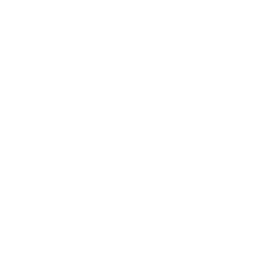
\includegraphics[scale=1]{assets/branding/opa0}
    \vspace{-5.75cm}\\
    {\adjustbox{scale=2.5}{\color{TealDarkCyan}\;I.\;Introduction}}
    \bigskip\bigskip
    {\ }\vspace{4cm}\\
    \bigskip
  \end{center}
\end{frame}

%--- Slide: Errors Are Everywhere ---
\begin{frame}[fragile]{\textbf{I. Introduction}}{Errors Are Everywhere}\small
\begin{columns}[T,onlytextwidth]
\begin{column}{.68\textwidth}
    \textcolor{TealDarkCyan}{\textbf{Physical world}}
    \begin{itemize}
      \item Scratches on a CD or DVD
    \end{itemize}
    \bigskip
    \textcolor{TealDarkCyan}{\textbf{Digital world}}
    \begin{itemize}
      \item Bit flips during internet transmission
    \end{itemize}
  \end{column}
  \begin{column}{.3\textwidth}
  	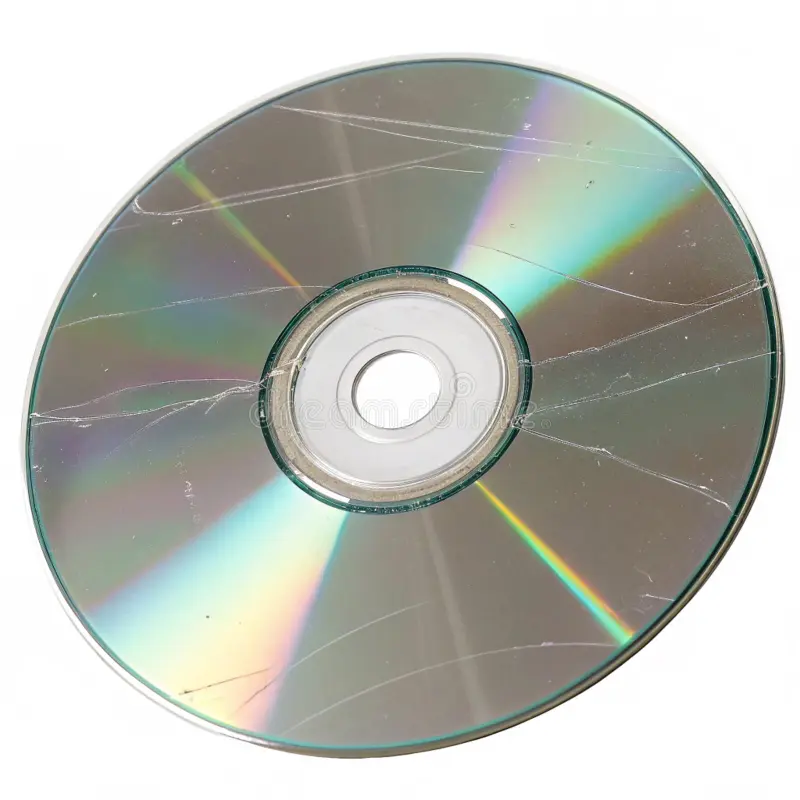
\includegraphics[scale=.1]{assets/image/scratched-cd}
\end{column}
\end{columns}
\vfill
\textbf{\color{red}Questions.} \begin{center}
	``How do we transmit (or store) data \textbf{reliably} in the presence of noise?''
\end{center}
\end{frame}

%--- Slide: Can We Make Noisy Data Reliable Again? ---
\begin{frame}[fragile]{\textbf{I. Introduction}}{Can We Make Noisy Data Reliable Again?}\small
\begin{center}
\begin{tikzpicture}[scale=0.92]
	% A simple "bit flip" picture
	\node[font=\ttfamily\large] at (0,3.0) {%
  $\cdots$1\,1\,1\,1\,0\,1\,1\,0\,1\,0\,1\,0\,1\,1\,0\,0\,1$\cdots$};
	\draw[-Stealth, thick, AccentCyan!70!black, dashed]
	(0,2.55) -- node[right=2pt,font=\footnotesize]{noise} (0,1.85);
	\node[font=\ttfamily\large] at (0,1.5) {%
  $\cdots$1\,1\,1\,1\,0\,1\,1\,0\,1\,0\,1\,0\,\textcolor{red!70!black}{0}\,1\,0\,0\,1$\cdots$};
\end{tikzpicture}
\end{center}
\bigskip
\begin{itemize}
	\item<2-> Can we \textbf{detect} it?
	\item[]
	\item<3-> Can we \textbf{fix} it?
\end{itemize}
\end{frame}

%%--- Slide: Familiar Example 1 — Check Digits ---
%\begin{frame}{\textbf{I. Introduction}}{A Familiar Example: Check Digits}
%\small
%Every ISBN-10 (International Standard Book Number) ends with a \textbf{check digit}.
%
%\medskip
%
%\textbf{Example.}\; ISBN $0\text{-}306\text{-}40615\text{-}2$: \begin{align*}
%&\; 1{\cdot}0 + 2{\cdot}3 + 3{\cdot}0 + 4{\cdot}6 + 5{\cdot}4 +\; 6{\cdot}0 + 7{\cdot}6 + 8{\cdot}1 + 9{\cdot}5 + 10{\cdot}2 \\
%=&\; 0+6+0+24+20+0+42+8+45+20 \\[2pt]
%=&\; 165 \;=\; 15\times11. \;\checkmark
%\end{align*}
%%\defbox[ISBN-10 check condition]{
%%For digits $d_1d_2\cdots d_{10}$ (where $d_{10}\in\{0,1,\ldots,9,X\}$, $X=10$), \[
%%  \sum_{i=1}^{10} i\cdot d_i \;\equiv\; 0 \pmod{11}.
%%\]}
%\textcolor{TealDarkCyan}{\textbf{What it guarantees}}
%\begin{itemize}
%	\item Detects \emph{every} single-digit error
%	\item Detects \emph{every} transposition of two adjacent digits
%\end{itemize}
%\bigskip
%\textcolor{AccentCyan!80!black}{\textbf{Limitation}}
%\begin{itemize}
%	\item One check digit $\Rightarrow$ detects errors, cannot \emph{correct} them
%\end{itemize}
%\end{frame}

%--- Slide: Repetition ---
\begin{frame}{\textbf{I. Introduction}}{Triple Repetition Code $\nkcode{3}{1}{2}$}
\small
The simplest way to correct errors: \textbf{say it three times}. \[
  \texttt{0} \;\longmapsto\; \texttt{000}, \qquad \texttt{1} \;\longmapsto\; \texttt{111}.
\]
%\medskip
%\defbox[Triple repetition code]{
%Encode one bit by repeating it three times:
%\[
%  0 \;\longmapsto\; 000, \qquad 1 \;\longmapsto\; 111.
%\]%\textbf{Decoding rule (majority vote):} decide the bit that appears most often.
%}
\begin{center}
\begin{minipage}{.49\textwidth}\centering
\begin{tabular}{c|c|c}
	\textbf{Received} & \textbf{Majority} & \textbf{Decision} \\\hline
	\rowcolor{TealDarkCyan!8} $\texttt{000}$ & $\texttt{0} \times 3$ & $\texttt{0}$ \\
	$\texttt{001}$ & $\texttt{0} \times 2$ & $\texttt{0}$ \\
	\rowcolor{TealDarkCyan!8} $\texttt{010}$ & $\texttt{0} \times 2$ & $\texttt{0}$ \\
	$\texttt{100}$ & $\texttt{0} \times 2$ & $\texttt{0}$ \\
	\rowcolor{AccentCyan!10} $\texttt{011}$ & $\texttt{1} \times 2$ & $\texttt{1}$ \\
	$\texttt{101}$ & $\texttt{1} \times 2$ & $\texttt{1}$ \\
	\rowcolor{AccentCyan!10} $\texttt{110}$ & $\texttt{1} \times 2$ & $\texttt{1}$ \\
	$\texttt{111}$ & $\texttt{1} \times 3$ & $\texttt{1}$ \\
\end{tabular}
\end{minipage}
\begin{minipage}{.49\textwidth}\centering
\begin{tikzpicture}[scale=0.92, font=\scriptsize]
	\node[circle,draw=TealDarkCyan,fill=TealDarkCyan!22,minimum size=.56cm] (c0) at (0,0) {$\texttt{000}$};
	\node[circle,draw=TealDarkCyan,fill=AccentCyan!20,minimum size=.56cm] (c1) at (3,0) {$\texttt{111}$};
	
	\draw[TealDarkCyan!60,thick,dashed] (c0) circle (1cm);
	\draw[AccentCyan!60,thick,dashed] (c1) circle (1cm);
	
	\node[circle,draw=black,fill=white,minimum size=.56cm] (r1) at (0,1) {$\texttt{100}$};
	\node[circle,draw=black,fill=white,minimum size=.56cm] (r2) at (-1,0) {$\texttt{010}$};
	\node[circle,draw=black,fill=white,minimum size=.56cm] (r3) at (0,-1) {$\texttt{001}$};
	\node[circle,draw=black,fill=red!12,minimum size=.56cm] (w110) at (2,0) {$\texttt{110}$};
	
	\draw[black!50, thin] (c0) -- (r1) node[midway,right, font=\tiny]{$1$};
	\draw[black!50, thin] (c0) -- (r2) node[midway,above, font=\tiny]{$1$};
	\draw[black!50, thin] (c0) -- (r3) node[midway,right, font=\tiny]{$1$};
	\draw[red!60!black, thick] (c0) -- (w110) node[midway, above, font=\tiny]{$2$};
	\draw[red!60!black, thick] (w110) -- (c1) node[midway, above, font=\tiny]{$1$};
	
%	\node[font=\tiny] at (1.5,-1.75) {\textbf{2-bit flips from \(000\): \(110,101,011\notin\{000,111\}\)}};
%	\node[font=\tiny,TealDarkCyan] at (1.5,-2) {\textbf{$001,101,011,110\notin C\Rightarrow$ detected (not a codeword)}};
%	\node[font=\tiny,red!70!black] at (1.5,-2.25) {\textbf{$110$ is decoded to $111$}};
	
	\node[font=\tiny,TealDarkCyan!80!black,align=center] at (1.5,-1.75)
	{\textbf{2-bit errors are detectable, but not always correctable.}};
\end{tikzpicture}
\end{minipage}
\end{center}
\begin{columns}[T,onlytextwidth]
\begin{column}{.375\textwidth}
\textcolor{TealDarkCyan}{\textbf{Performance}}
\begin{itemize}
	\item Detects any two-bit flips
	\item Corrects any single-bit flip
\end{itemize}
\end{column}
\begin{column}{.55\textwidth}
\textcolor{AccentCyan!80!black}{\textbf{Cost}}
\begin{itemize}
	\item Rate $R = 1/3$: send $3$ bits to convey $1$ bit
	\item Very inefficient!
\end{itemize}
\end{column}
\end{columns}
\vfill
\textbf{\color{red}Question.}\; Can we do much better?
\end{frame}

%--- Slide: Distance Intuition ---
\begin{frame}{\textbf{I. Introduction}}{The Key Idea: Distance}
\small
Why does the triple repetition code work? The two codewords are \textbf{far apart}.

\medskip
\begin{center}
\begin{minipage}{.49\textwidth}\centering
\begin{tikzpicture}[scale=0.95]
	% 3-cube nodes — explicit (no \foreach with color params to avoid xcolor whitespace bug)
	\node[circle,draw=TealDarkCyan,fill=TealDarkCyan!20,minimum size=.56cm,font=\scriptsize,inner sep=1pt] (v000) at (0.0, 0.0) {$000$};
	\node[circle,draw=TealDarkCyan,fill=white,           minimum size=.56cm,font=\scriptsize,inner sep=1pt] (v100) at (2.0, 0.0) {$100$};
	\node[circle,draw=TealDarkCyan,fill=white,           minimum size=.56cm,font=\scriptsize,inner sep=1pt] (v010) at (1.0, 0.9) {$010$};
	\node[circle,draw=TealDarkCyan,fill=white,           minimum size=.56cm,font=\scriptsize,inner sep=1pt] (v110) at (3.0, 0.9) {$110$};
	\node[circle,draw=TealDarkCyan,fill=white,           minimum size=.56cm,font=\scriptsize,inner sep=1pt] (v001) at (0.5, 1.6) {$001$};
	\node[circle,draw=TealDarkCyan,fill=white,           minimum size=.56cm,font=\scriptsize,inner sep=1pt] (v101) at (2.5, 1.6) {$101$};
	\node[circle,draw=TealDarkCyan,fill=white,           minimum size=.56cm,font=\scriptsize,inner sep=1pt] (v011) at (1.5, 2.5) {$011$};
	\node[circle,draw=TealDarkCyan,fill=TealDarkCyan!20,minimum size=.56cm,font=\scriptsize,inner sep=1pt] (v111) at (3.5, 2.5) {$111$};
	% Edges
	\foreach \a/\b in {v000/v001,v111/v011,v111/v101,v001/v011,v001/v101,v101/v100,v110/v110}
	\draw[TealDarkCyan!40] (\a)--(\b);
	\foreach \a/\b in {v000/v100,v111/v110,v100/v110}
	\draw[red] (\a)--(\b);
	\foreach \a/\b in {v000/v010,v010/v110,v010/v011}
	\draw[TealDarkCyan!40,dashed] (\a)--(\b);
	% Labels
	\node[above=2pt of v000,font=\scriptsize,TealDarkCyan]{\textbf{codeword}};
	\node[above=2pt of v111,font=\scriptsize,TealDarkCyan]{\textbf{codeword}};
\end{tikzpicture}
\end{minipage}\hfill
\begin{minipage}{.49\textwidth}
\begin{tikzpicture}[scale=0.92, font=\scriptsize]
	\tikzset{
		bitnode/.style={circle,draw=TealDarkCyan,minimum size=.56cm,fill=white},
		codeword/.style={circle,draw=TealDarkCyan,minimum size=.68cm,fill=TealDarkCyan!18}
	}
	%\draw[TealDarkCyan!40, very thick] (0,0.75) ellipse (4cm and 2.25cm);
	\node[codeword] (v000) at (-1.5,0.45) {\(000\)};
	\node[codeword] (v111) at (1.5,0.45) {\(111\)};
	
	\draw[TealDarkCyan!75, very thick, dashed] (v000) circle (1cm);
	\draw[TealDarkCyan!75, very thick, dashed] (v111) circle (1cm);
	
	\node[bitnode] (v001) at (-2.5,.45) {\(001\)};
	\node[bitnode] (v010) at (-1.5,1.45) {\(010\)};
	\node[bitnode] (v100) at (-1.5,-0.5) {\(100\)};
	
	\node[bitnode] (v110) at (1.5,-0.5) {\(110\)};
	\node[bitnode] (v101) at (1.5,1.45) {\(101\)};
	\node[bitnode] (v011) at (2.5,.45) {\(011\)};
	
	\draw[green!60!black,-Latex] (v001) -- (v000);
	\draw[green!60!black,-Latex] (v010) -- (v000);
	\draw[green!60!black,-Latex] (v100) -- (v000);
	\draw[green!60!black,-Latex] (v110) -- (v111);
	\draw[green!60!black,-Latex] (v101) -- (v111);
	\draw[green!60!black,-Latex] (v011) -- (v111);
	
	\node[font=\tiny,green!70!black,align=center,text width=2.8cm] at (-1.5,2.25)
	{\textbf{1-bit errors\\correct to \(000\)}};
	\node[font=\tiny,green!70!black,align=center,text width=2.8cm] at (1.5,2.25)
	{\textbf{1-bit errors\\correct to \(111\)}};
	\draw[red,Latex-Latex] (v000) -- (v111) node[midway,above] {$3$};
\end{tikzpicture}
\end{minipage}
\end{center}
\vfill
\defbox[Minimum distance]{
A code with minimum distance $d$ corrects all errors of weight $\displaystyle\le\left\lfloor\frac{(d-1)}{2}\right\rfloor$.
}
\end{frame}


%--- Slide: Distance Meaning I ---
\begin{frame}{\textbf{I. Introduction}}{Hamming Distance}
\small
Hamming distance counts how many coordinates differ. For any $\mathbf{x},\mathbf{y}\in\F_2^n$, \[
  d_H(\mathbf{x},\mathbf{y})=
  w_H(\mathbf{x}\oplus\mathbf{y})=\#\{i:\ x_i\neq y_i\}
\] where \(w_H\) is Hamming weight (number of ones).
\medskip

\begin{center}
\begin{tikzpicture}[scale=0.95]
	% Two strings with differences highlighted
	\foreach \i/\a/\b in {1/1/1, 2/0/1, 3/1/0, 4/1/1, 5/0/0, 6/0/1, 7/1/1} {
		\pgfmathsetmacro{\xpos}{(\i-1)*0.9}
		\ifnum\a=\b
		\node[minimum size=0.75cm, draw=TealDarkCyan!40, rounded corners=3pt,
		fill=TealDarkCyan!8, font=\small] at (\xpos, 0.6) {$\a$};
		\node[minimum size=0.75cm, draw=TealDarkCyan!40, rounded corners=3pt,
		fill=TealDarkCyan!8, font=\small] at (\xpos,-0.6) {$\b$};
		\else
		\node[minimum size=0.75cm, draw=AccentCyan, thick, rounded corners=3pt,
		fill=AccentCyan!18, font=\small\bfseries] at (\xpos, 0.6) {$\a$};
		\node[minimum size=0.75cm, draw=AccentCyan, thick, rounded corners=3pt,
		fill=AccentCyan!18, font=\small\bfseries] at (\xpos,-0.6) {$\b$};
		\draw[AccentCyan, thick, <->] (\xpos,0.22) -- (\xpos,-0.22)
		node[midway,right=1pt,font=\tiny]{$\neq$};
		\fi
	}
	\node[left=4pt, font=\small] at (-0.4, 0.6) {$x=$};
	\node[left=4pt, font=\small] at (-0.4,-0.6) {$y=$};
	\node[right=4pt, font=\small, TealDarkCyan] at (6, 0) {$d(x,y)=3$};
\end{tikzpicture}
\end{center}

\noindent
\textbf{Example 1.}\; \(d_H(0101,1100)=2\).
\medskip

\textbf{Example 2.}\; \(d_H(000,101)=2\).

\vfill

\textcolor{TealDarkCyan}{\textbf{Hamming distance is a metric}.} 
%\begin{enumerate}[(i)]
%	\item $d_H(\mathbf{x},\mathbf{y})\ge 0,
%	\ d_H(\mathbf{x},\mathbf{y})=0 \iff \mathbf{x}=\mathbf{y},$
%	\item $  d_H(\mathbf{x},\mathbf{y}) = d_H(\mathbf{y},\mathbf{x}),$
%	\item $d_H(\mathbf{x},\mathbf{z}) \le d_H(\mathbf{x},\mathbf{y}) + d_H(\mathbf{y},\mathbf{z}).$
%\end{enumerate}
\end{frame}

%--- Slide: Correction Balls ---
\begin{frame}{\textbf{I. Introduction}}{Correction Balls}
\small
\begin{center}
\begin{tikzpicture}[scale=0.95, font=\scriptsize]
\tikzset{
	cnode/.style={circle,draw=TealDarkCyan,fill=TealDarkCyan!18,minimum size=.64cm,very thick},
	grid/.style={line width=.6pt}
}
\foreach \i/\x/\y/\L in {
	1/-4/ 1.5/{$c_1$},
	2/-3/ -2/{$c_2$},
	3/0/ 0/{$c_3$},
	4/3/ 1.70/{$c_4$},
	5/4/-1.25/{$c_5$}
}{
	\node[cnode] (c\i) at (\x,\y) {\L};
}
\node[cnode, draw=red, fill=red!20] at (1,1) {};
\node[cnode, draw=red, fill=red!20] at (2,-1) {};
\node[cnode, draw=red, fill=red!20] at (-1.75,-.5) {};
\node[cnode, draw=red, fill=red!20] at (-2.75,.5) {};
\node[cnode, draw=red, fill=red!20] at (2,1.25) {};
\only<2>{\foreach \i in {1,...,5} {\draw[TealDarkCyan,dashed, thick] (c\i) circle (1cm);}}
\only<3>{\foreach \i in {1,...,5} {\draw[TealDarkCyan,dashed, very thick] (c\i) circle (1.5cm);}}
\only<4>{\foreach \i in {1,...,5} {\draw[Red!70!black,dashed, very thick] (c\i) circle (1.75cm);}}
\end{tikzpicture}
\end{center}
\only<4>{\textbf{Remark.}\; \textcolor{TealDarkCyan}{\textbf{No overlap of correction balls} $\;\Longleftrightarrow\;$ unique decoding is possible.}}
\end{frame}

%%--- Slide: QR Codes ---
%\begin{frame}{\textbf{I. Introduction}}{Real-World Example: QR Codes}
%\small
%\begin{columns}[T,onlytextwidth]
%  \begin{column}{.54\textwidth}
%    QR codes use \textbf{Reed--Solomon error correction} — a powerful algebraic code.
%
%    \bigskip
%    \defbox[Four error-correction levels]{
%    \begin{tabular}{c|l|l}
%      \textbf{Level} & \textbf{Recovery} & \textbf{Use case} \\\hline
%      L & up to $7\%$ & clean environments\\
%      M & up to $15\%$ & standard use\\
%      Q & up to $25\%$ & industrial\\
%      H & up to $30\%$ & high damage risk
%    \end{tabular}
%    }
%
%    \bigskip
%    \textcolor{TealDarkCyan}{\textbf{Why Reed--Solomon?}}
%    \begin{itemize}
%      \item Designed for \emph{burst errors} (adjacent damage)
%      \item Algebraic structure enables fast decoding
%      \item Same code used in CDs, DVDs, Blu-ray
%    \end{itemize}
%  \end{column}
%  \begin{column}{.43\textwidth}
%    \begin{center}
%    \begin{tikzpicture}[scale=0.85]
%      % Draw a schematic QR-code grid
%      \foreach \x in {0,...,6}
%        \foreach \y in {0,...,6}
%          \fill[TealDarkCyan!15] (\x*0.35, \y*0.35) rectangle ++(0.32,0.32);
%      % Finder patterns (top-left)
%      \fill[TealDarkCyan]    (0,6*0.35) rectangle ++(7*0.35,0.35);
%      \fill[TealDarkCyan]    (0,0) rectangle ++(7*0.35,0.35);
%      \fill[TealDarkCyan]    (0,0) rectangle ++(0.35,7*0.35);
%      \fill[TealDarkCyan]    (6*0.35,0) rectangle ++(0.35,7*0.35);
%      \fill[white]           (0.35,0.35) rectangle ++(5*0.35,5*0.35);
%      \fill[TealDarkCyan]    (0.7,0.7) rectangle ++(3*0.35,3*0.35);
%      % A "damage" patch
%      \fill[AccentCyan!35]   (1.2,1.15) rectangle ++(0.9,0.9);
%      \node[font=\tiny, AccentCyan!80!black] at (1.65,1.6) {damage};
%      % Label
%      \node[font=\footnotesize, TealDarkCyan] at (1.225,-0.3)
%        {still readable!};
%    \end{tikzpicture}
%    \end{center}
%    \bigskip
%    \begin{block}{}
%    \centering\small
%    Up to $30\%$ of a QR code can be destroyed and it still decodes correctly.
%    \end{block}
%  \end{column}
%\end{columns}
%\end{frame}

%--- Slide: The Communication Problem ---
\begin{frame}{\textbf{I. Introduction}}{The Communication Model}
\begin{center}
\begin{tikzpicture}[
>=Stealth,
block/.style={
	draw=TealDarkCyan, thick, fill=AccentCyan!80!black, rounded corners=2mm,
	minimum width=1.2cm, minimum height=1cm, align=center,
	font=\sffamily, drop shadow={opacity=0.15, shadow xshift=1mm, shadow yshift=-1mm}
},
adder/.style={
	circle, draw=TealDarkCyan, thick, fill=AccentCyan!80!black,
	minimum size=6mm, inner sep=0pt, align=center, font=\Large,
	drop shadow={opacity=0.15, shadow xshift=1mm, shadow yshift=-1mm}
},
arrow/.style={->, thick, TealDarkCyan},
mathlabel/.style={font=\normalsize, text=black},
sublabel/.style={font=\small\sffamily, text=magenta},
scale=.75
]

% Invisible nodes to act as the start and end points of the signals
\node (start) at (0,0) {};
\node (end)   at (19,0) {};

% Main operational blocks
\node[block, align=center, font=\color{white}] (enc) at (4.5,0) {Encoder\\ $\F_2^k\to\F_2^n$};
\onslide<2->\node[adder, font=\color{white}] (add) at (9.5,0) {$+$};
\onslide<3->\node[block, align=center, font=\color{white}] (dec) at (14.5,0) {Decoder\\ $\F_2^n\to\F_2^k$};

% Noise entry point
\onslide<2->\node (noise) at (9.5, 2) {\small \texttt{Noise} $\vect{e}$};

% --- Signal Paths & Labels ---

% Source to Encoder
\onslide<1->\draw[arrow] (start) -- 
node[midway, mathlabel, draw=TealDarkCyan, fill=white, align=center] {\texttt{message}\\ [-1.25mm] $\vect{x}$} node[below=5mm, sublabel] {$k$-bit} (enc);

% Encoder to Channel (Adder)
% We use a standard label below the arrow to replace the underbrace in the equation
\onslide<1->\draw[arrow] (enc) -- 
node[midway, mathlabel, draw=TealDarkCyan, fill=white, align=center] {\texttt{codeword}\\ [-1.25mm] $\vect{c}$} node[below=5mm, sublabel] {$n$-bit ($n>k$)} (add);

% Noise entering the Channel
\onslide<2->\draw[arrow] (noise) -- (add);

% Channel to Decoder
\onslide<2->\draw[arrow] (add) -- 
node[midway, mathlabel, draw=TealDarkCyan, fill=white, align=center] {\texttt{received}\\ [-1.25mm]  \texttt{vector} $\vect{y}$} node[below=5mm, sublabel] {$n$-bit} (dec);

% Decoder to Destination
\onslide<3->\draw[arrow] (dec) -- 
node[midway, mathlabel, draw=TealDarkCyan, fill=white, align=center] {\texttt{message}\\ [-1.25mm] $\widehat{\vect{x}}$} node[below=5mm, sublabel] {$k$-bit} (end);

\onslide<2->\draw[dashed, red] (8.7,-1.2) rectangle (10.3,2.5);
\onslide<2->\node[red] at (9.5,3) {channel};
\end{tikzpicture}
\end{center}
%\begin{center}
%\begin{tikzpicture}[
%  cbox/.style   = {draw, thick, rounded corners=4pt, minimum height=.85cm,
%                   minimum width=1.8cm, align=center},
%  arr/.style    = {-Stealth, thick, color=TealDarkCyan},
%  noise/.style  = {-Stealth, thick, color=AccentCyan!80!black},
%  lbl/.style    = {font=\small}
%]
%  \node[cbox, fill=TealDarkCyan!15] (src) {\small Source\\[-2pt]$\mathbf{m}$};
%  \node[cbox, fill=TealDarkCyan!25, right=1.1cm of src]  (enc) {\small Encoder};
%  \node[cbox, fill=AccentCyan!18,    right=1.1cm of enc]  (ch)  {\small Noisy\\[-2pt]\small Channel};
%  \node[cbox, fill=TealDarkCyan!25, right=1.1cm of ch]   (dec) {\small Decoder};
%  \node[cbox, fill=TealDarkCyan!15, right=1.1cm of dec]  (dst) {\small Receiver\\[-2pt]$\hat{\mathbf{m}}$};
%  \node[above=.55cm of ch, AccentCyan!80!black]    (err) {\small $\mathbf{e}$\; (noise)};
%
%  \draw[arr] (src) -- (enc) node[midway,above,lbl]{$\mathbf{m}$};
%  \draw[arr] (enc) -- (ch)  node[midway,above,lbl]{$\mathbf{c}$};
%  \draw[arr] (ch)  -- (dec) node[midway,above,lbl]{$\mathbf{v}=\mathbf{c}+\mathbf{e}$};
%  \draw[arr] (dec) -- (dst) node[midway,above,lbl]{$\hat{\mathbf{m}}$};
%  \draw[noise] (err) -- (ch);
%\end{tikzpicture}
%\end{center}
\bigskip
\begin{columns}[T,onlytextwidth]
\begin{column}{.4\textwidth}
\textbf{Setup}
\begin{itemize}\small
	\item Message $\mathbf{x}\in\F_q^k$
	\item Encoder : $\mathbf{x}\mapsto\mathbf{c}\in\F_q^n$,\; $n>k$
	\item Channel : $\mathbf{y}=\mathbf{c}\oplus\mathbf{e}$
\end{itemize}
\end{column}
\begin{column}{.58\textwidth}
\textbf{Goal}
	\begin{itemize}\small
	\item Recover $\hat{\mathbf{x}}=\mathbf{x}$ even when $\mathbf{e}\neq\mathbf{0}$
	\item Keep rate $R = k/n$ as large as possible
	\end{itemize}
\end{column}
\end{columns}
\end{frame}

%--- Slide: The Rate--Distance Tradeoff ---
\begin{frame}{\textbf{I. Introduction}}{The Fundamental Tradeoff}\small
\begin{center}\renewcommand{\arraystretch}{1.25}
\begin{tabular}{l|ccc}
	\textbf{Code} & \textbf{Rate} & \textbf{Detects} & \textbf{Corrects} $t$\\\hline
	$\nkdcode{n}{k}{d}{q}$-code & $k/n$&  $d-1$ & $\left\lfloor(d-1)/2\right\rfloor$\\\hline
	Repetition $\nkdcode{3}{1}{3}{2}$ & $1/3\approx0.33$ & 2 & 1 \\
	Hamming $[7,4,3]_2$ & $4/7\approx 0.57$ & 2 & 1 \\
	BCH $[15,7,5]_2$ & $7/15\approx 0.47$ & 4 & 2 \\
	Reed-Solomon $[15,11,5]_{16}$ & $11/15\approx 0.73$ & 4 & 2 \\
	Reed-Solomon $[255,223,33]_{256}$ & $223/255\approx 0.87$ & 32 & 16 \\
\end{tabular}
\end{center}
\begin{itemize}
	\item high rate $\implies$ efficiency
	\item correct many errors $\implies$ powerful
\end{itemize}
%\vspace{-2pt}
%\begin{center}
%\begin{tikzpicture}[x=7.6cm, y=1.25cm, font=\scriptsize]
%	% light grid
%	\draw[thin,gray!22] (0,0) grid[xstep=0.2,ystep=1] (1.0,2.7);
%	% axes
%	\draw[-Stealth,thick,TealDarkCyan] (-0.018,0) -- (1.10,0)
%	node[right,font=\small]{Rate $R=k/n$};
%	\draw[-Stealth,thick,TealDarkCyan] (0,-0.18) -- (0,3.05)
%	node[above,font=\small]{Correctable errors $t$};
%	% x ticks
%	\foreach \x in {0.2,0.4,0.6,0.8,1.0}
%	\draw[gray!60] (\x,0)--++(0,-0.12)
%	  node[below=1pt,font=\tiny]{\pgfmathprintnumber[fixed,precision=1]{\x}};
%	% y ticks
%	\foreach \y in {1,2}
%	\draw[gray!60] (0,\y)--++(-0.016,0) node[left=1pt,font=\tiny]{$\y$};
%%	% Singleton bound for n=15: t = 7.5(1-R)
%%	% enters plot at R=1-2.7/7.5=0.64; hits zero at R=1
%%	\draw[AccentCyan!75!black, dashed, thick] (0.64,2.7) -- (1.0,0);
%%	\node[AccentCyan!75!black, font=\tiny, rotate=-73, anchor=center] at (0.845,1.35)
%%	{Singleton ($n\!=\!15$)};
%	% ---- binary code points (TealDarkCyan) ----
%	% Repetition [3,1,3]_2  R=1/3, t=1
%	\fill[TealDarkCyan] (0.3333,1) circle (2.6pt);
%	\node[above=3pt, TealDarkCyan, align=center] at (0.3333,1)
%	{Rep.\ $[3,1,3]_2$};
%	% BCH [15,7,5]_2  R=7/15, t=2
%	\fill[TealDarkCyan] (0.4667,2) circle (2.6pt);
%	\node[left=4pt, TealDarkCyan, align=right] at (0.4667,2)
%	{BCH $[15,7,5]_2$};
%	% Hamming [7,4,3]_2  R=4/7, t=1
%	\fill[TealDarkCyan] (0.5714,1) circle (2.6pt);
%	\node[below=3pt, TealDarkCyan, align=center] at (0.5714,1)
%	{Ham.\ $[7,4,3]_2$};
%  % ---- RS [15,11,5]_{16}  R=11/15, t=2  (MDS: sits on Singleton line) ----
%  \fill[AccentCyan!80!black] (0.7333,2) circle (3.2pt);
%%  \draw[AccentCyan!80!black, thick] (0.7333,2) circle (4.8pt);
%  \node[right=4pt, AccentCyan!80!black, align=center] at (0.7333,2)
%    {RS $[15,11,5]_{16}$\;%\textbf{(MDS)}
%    };
%%  % tradeoff arrow annotation
%%  \draw[-Stealth,gray!55,thin] (0.16,2.55) -- (0.90,0.25);
%%  \node[gray!65, font=\tiny, rotate=-68, anchor=center] at (0.47,1.55)
%%    {more redundancy $\to$ more correction};
%\end{tikzpicture}
%\end{center}
\end{frame}

%%--- Slide: Shannon's Theorem ---
%\begin{frame}{\textbf{I. Introduction}}{Shannon's Channel Coding Theorem (1948)}
%
%\defbox[Shannon's Channel Coding Theorem]{
%For any discrete memoryless channel with capacity $C$ and any rate $R<C$, there exists a sequence of codes of rate $\to R$ whose block error probability $\to 0$.
%}
%
%\bigskip
%\begin{columns}[T,onlytextwidth]
%  \begin{column}{.48\textwidth}
%    \textcolor{TealDarkCyan}{\textbf{What it guarantees}}
%    \begin{itemize}\small
%      \item Reliable communication \emph{is} possible below capacity
%      \item Error probability can be made arbitrarily small
%      \item A fundamental \emph{existence} result
%    \end{itemize}
%  \end{column}
%  \begin{column}{.48\textwidth}
%    \textcolor{AccentCyan!80!black}{\textbf{What it does not provide}}
%    \begin{itemize}\small
%      \item \emph{How} to construct such codes explicitly
%      \item \emph{How} to decode efficiently
%      \item The proof uses random codes!
%    \end{itemize}
%  \end{column}
%\end{columns}
%
%\bigskip
%\begin{alertblock}{The Central Challenge of Coding Theory}
%\centering
%Construct \textbf{explicit algebraic codes} that are both \textbf{efficient} (high rate) and \textbf{powerful} (correct many errors).
%\end{alertblock}
%\end{frame}

%%--- Slide: History Overview ---
%\begin{frame}{\textbf{I. Introduction}}{A Brief History of Error-Correcting Codes}
%\small
%\begin{columns}[T,onlytextwidth]
%\begin{column}{.56\textwidth}
%\begin{tikzpicture}[x=1cm, y=0.60cm, font=\scriptsize]
%  \draw[thick, gray!35] (0,8.8)--(0,0);
%  % Classical era sidebar (1948--1970)
%  \draw[TealDarkCyan!55, line width=2.8pt] (-0.22,8.7)--(-0.22,3.55);
%  \node[rotate=90, font=\tiny, TealDarkCyan!70] at (-0.44,6.15) {Classical era};
%  % Modern era sidebar
%  \draw[AccentCyan!65, line width=2.8pt] (-0.22,3.3)--(-0.22,0.0);
%  \node[rotate=90, font=\tiny, AccentCyan!80!black] at (-0.44,1.65) {Modern era};
%  % 1948
%  \fill[AccentCyan!80!black] (0,8.5) circle (2.3pt);
%  \draw[thin,AccentCyan!80!black] (0,8.5)--(0.18,8.5);
%  \node[right=2pt, AccentCyan!80!black, align=left] at (0.18,8.5)
%    {\textbf{1948} \textit{Shannon} --- capacity theorem (Bell Labs)};
%  % 1950
%  \fill[TealDarkCyan] (0,7.5) circle (2.3pt);
%  \draw[thin,TealDarkCyan] (0,7.5)--(0.18,7.5);
%  \node[right=2pt, TealDarkCyan, align=left] at (0.18,7.5)
%    {\textbf{1950} \textit{Hamming} --- $[7,4,3]_2$, first perfect code};
%  % 1954
%  \fill[TealDarkCyan] (0,6.5) circle (2.3pt);
%  \draw[thin,TealDarkCyan] (0,6.5)--(0.18,6.5);
%  \node[right=2pt, TealDarkCyan, align=left] at (0.18,6.5)
%    {\textbf{1954} \textit{Reed, Muller} --- polynomial evaluation codes};
%  % 1959-60
%  \fill[TealDarkCyan] (0,5.5) circle (2.3pt);
%  \draw[thin,TealDarkCyan] (0,5.5)--(0.18,5.5);
%  \node[right=2pt, TealDarkCyan, align=left] at (0.18,5.5)
%    {\textbf{1959/60} \textit{BCH \& Reed--Solomon} --- designed distance};
%  % 1963
%  \fill[TealDarkCyan] (0,4.5) circle (2.3pt);
%  \draw[thin,TealDarkCyan] (0,4.5)--(0.18,4.5);
%  \node[right=2pt, TealDarkCyan, align=left] at (0.18,4.5)
%    {\textbf{1963} \textit{Gallager} --- LDPC (hardware not yet ready)};
%  % 1970
%  \fill[TealDarkCyan] (0,3.85) circle (2.3pt);
%  \draw[thin,TealDarkCyan] (0,3.85)--(0.18,3.85);
%  \node[right=2pt, TealDarkCyan, align=left] at (0.18,3.85)
%    {\textbf{1970} \textit{Goppa} --- classical Goppa codes; AG codes (1982)};
%  % 1993
%  \fill[AccentCyan!80!black] (0,3.2) circle (2.3pt);
%  \draw[thin,AccentCyan!80!black] (0,3.2)--(0.18,3.2);
%  \node[right=2pt, AccentCyan!80!black, align=left] at (0.18,3.2)
%    {\textbf{1993} \textit{Berrou et al.} --- Turbo codes; near-capacity; 3G/4G};
%  % 1995
%  \fill[AccentCyan!80!black] (0,2.2) circle (2.3pt);
%  \draw[thin,AccentCyan!80!black] (0,2.2)--(0.18,2.2);
%  \node[right=2pt, AccentCyan!80!black, align=left] at (0.18,2.2)
%    {\textbf{1995} \textit{MacKay \& Neal} --- LDPC revived; 5G/Wi-Fi};
%  % 2009
%  \fill[AccentCyan!80!black] (0,1.1) circle (2.3pt);
%  \draw[thin,AccentCyan!80!black] (0,1.1)--(0.18,1.1);
%  \node[right=2pt, AccentCyan!80!black, align=left] at (0.18,1.1)
%    {\textbf{2009} \textit{Ar{\i}kan} --- polar codes; first proven capacity-achieving};
%\end{tikzpicture}
%\end{column}
%\begin{column}{.41\textwidth}
%  \textcolor{TealDarkCyan}{\textbf{Classical era (1948--1970)}}
%  \begin{itemize}\small
%    \item Shannon's proof uses random codes — non-constructive
%    \item Algebra provides \emph{explicit} efficient constructions
%    \item Tools: finite fields, polynomial rings, algebraic geometry
%  \end{itemize}
%  \smallskip
%  \textcolor{AccentCyan!80!black}{\textbf{Modern era (1993--2009)}}
%  \begin{itemize}\small
%    \item \textbf{$\approx$30-year gap:} Goppa AG (1982) $\to$ near-capacity (1993)
%    \item Breakthrough: iterative belief-propagation on graphs
%    \item Polar codes (2009): \emph{provably} achieve capacity
%  \end{itemize}
%\end{column}
%\end{columns}
%\end{frame}
%
%%--- Slide: Classical Era ---
%\begin{frame}{\textbf{I. Introduction}}{The Classical Era (1948--1963)}\small
%\begin{columns}[T,onlytextwidth]
%\begin{column}{.49\textwidth}
%
%\defbox[Hamming Codes (1950)]{
%\scriptsize
%\begin{itemize}
%  \item[$\bullet$] \textbf{Context:} R.\,Hamming (Bell Labs) was frustrated that weekend batch jobs crashed on single parity errors — he automated the fix
%  \item[$\bullet$] $[7,4,3]_2$: 3 redundancy bits protect 4 data bits; a \emph{perfect code} — correction balls partition $\F_2^7$ exactly
%  \item[$\bullet$] Introduced Hamming distance $d_H$ and weight $w_H$, the core metrics of all coding theory
%\end{itemize}
%}
%
%\smallskip
%
%\defbox[BCH Codes (1959--60)]{
%\scriptsize
%\begin{itemize}
%  \item[$\bullet$] Hocquenghem (1959) and Bose--Ray-Chaudhuri (1960) independently
%  \item[$\bullet$] Roots $\alpha,\alpha^2,\ldots,\alpha^{d-1}$ of $g(X)$ guarantee $d_{\min}\ge d$: first family with \emph{designed} minimum distance
%  \item[$\bullet$] Berlekamp--Massey $O(n^2)$ decoder; \textbf{used in:} CDs, flash, QR codes
%\end{itemize}
%}
%
%\end{column}
%\begin{column}{.49\textwidth}
%
%\defbox[Reed--Muller Codes (1954)]{
%\scriptsize
%\begin{itemize}
%  \item[$\bullet$] Codewords = evaluations of degree-${\le}r$ polynomials over $\F_2^m$; length $2^m$, distance $2^{m-r}$
%  \item[$\bullet$] Recursive $(\mathbf{u}\mid\mathbf{u}{+}\mathbf{v})$ construction enables simple majority-logic decoding
%  \item[$\bullet$] \textbf{Application:} Mariner~9 (1972) used $\mathcal{R}(1,5)$ — rate $6/32$, corrects $\le 7$ errors — to transmit the first Mars photos; precursor of polar codes
%\end{itemize}
%}
%
%\smallskip
%
%\defbox[Reed--Solomon Codes (1960)]{
%\scriptsize
%\begin{itemize}
%  \item[$\bullet$] Codewords = evaluations of degree-$<k$ polynomials at $n$ distinct points over $\F_q$
%  \item[$\bullet$] \emph{MDS codes}: achieve Singleton bound $d=n{-}k{+}1$; optimal burst-error correction
%  \item[$\bullet$] \textbf{Used in:} CDs/DVDs, Voyager~1\&2, RAID, QR codes, DSL
%\end{itemize}
%}
%
%\end{column}
%\end{columns}
%\end{frame}
%
%%--- Slide: Goppa Codes ---
%\begin{frame}{\textbf{I. Introduction}}{Goppa Codes: From Polynomial Roots to Algebraic Curves}\small
%\begin{columns}[T,onlytextwidth]
%\begin{column}{.49\textwidth}
%
%\defbox[Classical Goppa Codes (V.\,D.\,Goppa, 1970)]{
%\scriptsize
%\begin{itemize}
%  \item[$\bullet$] Fix $g(z)\in\F_{q^m}[z]$ of degree $t$ and $L=\{\alpha_1,\ldots,\alpha_n\}\subset\F_{q^m}$. The Goppa code $\Gamma(L,g)$ consists of all $\mathbf{c}\in\F_q^n$ satisfying \[
%  \textstyle\sum_{i=1}^{n}\frac{c_i}{z-\alpha_i}\;\equiv\;0\pmod{g(z)}
%  \]
%  \item[$\bullet$] Parameters: $[n,\;k\ge n-mt,\;d\ge t+1]_q$; binary irreducible Goppa codes achieve $d\ge 2t+1$ (double the BCH guarantee)
%  \item[$\bullet$] Strictly generalise BCH (take $g=(z-\alpha)^t$) and Reed--Solomon codes
%  \item[$\bullet$] \textbf{McEliece (1978):} first code-based public-key cryptosystem using binary Goppa codes; quantum-resistant — a leading NIST post-quantum candidate
%\end{itemize}
%}
%
%\end{column}
%\begin{column}{.49\textwidth}
%
%\defbox[Algebraic Geometry Codes (1977--1982)]{
%\scriptsize
%\begin{itemize}
%  \item[$\bullet$] \textbf{Goppa (1977/1981):} encode information as evaluations of rational functions from the Riemann--Roch space $L(G)$ on an algebraic curve $\mathcal{X}/\F_q$; length $n = |\mathcal{X}(\F_q)|$
%  \item[$\bullet$] Parameters satisfy $k+d\ge n+1-g$ (Riemann--Roch lower bound), where $g$ = genus; genus 0 recovers Reed--Solomon
%  \item[$\bullet$] \textbf{Tsfasman--Vladut--Zink (1982):} using Shimura modular curves, first codes ever proven to \emph{exceed} the Gilbert--Varshamov bound (for $q=p^2\ge 49$)
%  \item[$\bullet$] Fused algebraic geometry with coding theory; opened an active research frontier
%\end{itemize}
%}
%
%\end{column}
%\end{columns}
%\end{frame}
%
%%--- Slide: Modern Era ---
%\begin{frame}{\textbf{I. Introduction}}{The Modern Era: Toward Shannon's Limit (1993--2009)}\small
%\begin{columns}[T,onlytextwidth]
%\begin{column}{.325\textwidth}
%
%\defbox[Turbo Codes (1993)]{
%\scriptsize
%\begin{itemize}
%  \item[$\bullet$] Berrou, Glavieux, Thitimajshima; announced at ICC 1993, met with initial skepticism
%  \item[$\bullet$] Two conv.\ codes + pseudo-random interleaver
%  \item[$\bullet$] Iterative soft (log-likelihood) belief exchange between two SISO decoders
%  \item[$\bullet$] First to reach within $0.5$ dB of Shannon limit
%  \item[$\bullet$] \textbf{Adopted in:} 3G (UMTS), 4G (LTE)
%\end{itemize}
%}
%
%\end{column}
%\begin{column}{.325\textwidth}
%
%\defbox[LDPC Codes (1963\,/\,1995)]{
%\scriptsize
%\begin{itemize}
%  \item[$\bullet$] \textbf{Gallager (1963):} sparse parity-check $H$; sum-product decoding conceived but ignored — 1960s computers too slow
%  \item[$\bullet$] \textbf{MacKay \& Neal (1995):} rediscovered; belief propagation on the Tanner graph now practical
%  \item[$\bullet$] Near-Shannon performance, low hardware complexity
%  \item[$\bullet$] \textbf{Adopted in:} 5G NR, Wi-Fi 802.11n, DVB-S2
%\end{itemize}
%}
%
%\end{column}
%\begin{column}{.325\textwidth}
%
%\defbox[Polar Codes (2009)]{
%\scriptsize
%\begin{itemize}
%  \item[$\bullet$] \textbf{Ar{\i}kan (2009):} \emph{channel polarization} — $n$ copies of $W$ split into ${\approx}nC$ near-perfect and ${\approx}n(1{-}C)$ near-useless sub-channels
%  \item[$\bullet$] First code \emph{proven} capacity-achieving for any symmetric channel; $O(n\log n)$ enc./dec.
%  \item[$\bullet$] SC decoding ($O(n\log n)$); SC-list improves finite-length performance
%  \item[$\bullet$] \textbf{Adopted in:} 5G NR control channel (eMBB)
%\end{itemize}
%}
%
%\end{column}
%\end{columns}
%\vfill
%\begin{alertblock}{}
%\centering\scriptsize
%\textbf{Common thread:} all three exploit iterative/belief-propagation decoding on graphical models to approach Shannon's bound.
%\end{alertblock}
%\end{frame}

%%--- Slide: Three Families We Study ---
%\begin{frame}{\textbf{I. Introduction}}{Three Beautiful Families}
%\small
%\begin{columns}[T,onlytextwidth]
%  \begin{column}{.47\textwidth}
%    \defbox[II. Linear Codes]{
%    \footnotesize
%    \begin{itemize}
%      \item[$\bullet$] Subspaces of $\F_q^n$; generator matrix $G$, parity-check $H$
%      \item[$\bullet$] Key bounds: Hamming, Singleton, Griesmer
%    \end{itemize}
%    }
%    \medskip
%    \defbox[III. Hamming Codes]{
%    \footnotesize
%    \begin{itemize}
%      \item[$\bullet$] Columns of $H$ = all nonzero points of $\mathrm{PG}(r-1,q)$
%      \item[$\bullet$] Perfect single-error-correcting codes
%    \end{itemize}
%    }
%    \medskip
%    \defbox[IV. Cyclic Codes]{
%    \footnotesize
%    \begin{itemize}
%      \item[$\bullet$] Ideals in $\F_q[X]/(X^n-1)$; generator polynomial $g(X)$
%      \item[$\bullet$] BCH codes: prescribed roots $\Rightarrow$ guaranteed distance
%    \end{itemize}
%    }
%  \end{column}
%\end{columns}
%\end{frame}

%--- Slide: Roadmap ---
\begin{frame}{\textbf{I. Introduction}}{Roadmap}
\defbox[II.\;Linear Codes]{
\small Structure via \textbf{linear algebra}
\begin{itemize}
	\item[$\bullet$] Subspaces of $\F_q^n$
	\item[$\bullet$] Generator Matrix $G$, parity-check $H$
	\item[$\bullet$] Hamming distance \& error correction
\end{itemize}}
%\defbox[III.\;Hamming Codes]{
%\small Perfect single-error correction
%Perfect codes via \textbf{projective geometry}
%\begin{itemize}
%	\item[$\bullet$] Parity checks from projective points
%	\item[$\bullet$] Syndrome decoding as geometry
%	\item[$\bullet$] Perfect single-error correction
%\end{itemize}
%}
\defbox[IV.\;Cyclic Codes]{
\small
Structure via \textbf{polynomial rings}
\begin{itemize}
	 \item[$\bullet$] Quotient $\F_q[X]/\langle X^n-1\rangle$
	 \item[$\bullet$] Ideals and generator polynomials
	 \item[$\bullet$] BCH design and cyclic Hamming codes
\end{itemize}
}
%    \begin{block}{Key Observation}
%    \small Coding theory is a meeting point of \textbf{linear algebra}, \textbf{finite geometry}, and \textbf{polynomial algebra}.
%    \end{block}
\end{frame}


%-------------------------------------------------------
% II. LINEAR CODES
%-------------------------------------------------------
\section{II. Linear Codes}
%=======================================================
% CHAPTER 1: LINEAR CODES
%=======================================================

\begin{frame}[plain]
  \begin{center}\bfseries\centering
    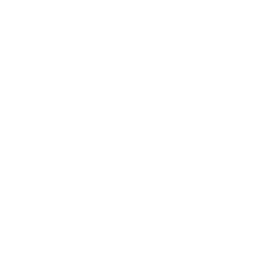
\includegraphics[scale=1]{assets/branding/opa0}
    \vspace{-5.75cm}\\
    {\adjustbox{scale=2.15}{\color{TealDarkCyan}\;II.\;Linear Codes}}
    \bigskip\bigskip
    {\ }\vspace{4cm}\\
    \bigskip
  \end{center}
\end{frame}


%%--- EXISTING FRAME RESTORED ---
%\begin{frame}{\textbf{II. Linear Codes}}{The ambient space}
%\small
%\defbox[Hamming space]{
%Fix a finite field $\F_q$. The set $\F_q^n$ is simultaneously a vector space and a metric space with
%\[
%  d(x,y)=\#\{i:x_i\ne y_i\}.
%\]
%}
%\begin{itemize}
%  \item The metric is translation invariant: $d(x+z,y+z)=d(x,y)$.
%  \item The spheres are combinatorial objects:
%  \[
%    |B_t(0)|=\sum_{i=0}^t \binom{n}{i}(q-1)^i.
%  \]
%  \item Coding theory asks for large subsets with large mutual distance.
%\end{itemize}
%\end{frame}

%\begin{frame}{\textbf{II. Linear Codes}}{Codes as metric subsets}
%\small
%\defbox[Code]{
%A code of length $n$ over $\F_q$ is a subset $\code\subseteq \F_q^n$. Its minimum distance is
%\[
%  d(\code)=\min\{d(x,y):x,y\in\code,\ x\ne y\}.
%\]
%}
%\begin{block}{Mathematician's viewpoint}
%The fundamental problem is an extremal problem in a finite metric space:
%\[
%  A_q(n,d)=\max\{|\code|:\code\subseteq\F_q^n,\ d(\code)\ge d\}.
%\]
%\end{block}
%\end{frame}

\begin{frame}{\textbf{II. Linear Codes}}{Linear Code}
\small
\defbox[Linear Encoding]{
\textbf{Definition.}\; A \textbf{linear encoding} over \(\F_q\) is a linear map
\[
\F_q^k \longrightarrow \F_q^n,
\qquad
\vect{x}\longmapsto \vect{c}.
\]}

\defbox[Linear code]{
\textbf{Definition.}\; A \textbf{linear $[n,k,d]_q$ code} is a $k$-dimensional subspace \[
\code\le \F_q^n
\] with minimum distance $d$. The elements of \(\code\) are called \textbf{codewords}.}
\end{frame}

%\begin{frame}{\textbf{II. Linear Codes}}{Weight}
%\small
%\defbox[Hamming weight]{
%For $x=(x_1,\ldots,x_n)\in\F_q^n$,
%\[
%  \wt(x)=|\supp(x)|,\qquad \supp(x)=\{i:x_i\ne0\}.
%\]
%}
%\begin{block}{Lemma}
%For a linear code $\code$,
%\[
%  d(\code)=\min_{0\ne c\in\code}\wt(c).
%\]
%\end{block}
%\textbf{Proof.} If $x,y\in\code$, then $x-y\in\code$ and $d(x,y)=\wt(x-y)$.
%\end{frame}

%--- Slide: Generator Matrices ---
\begin{frame}{\textbf{II. Linear Codes}}{Generator Matrices}
\small
\defbox[Generator matrix]{
\textbf{Definition.}\; A \textbf{generator matrix} for an $\nkcode{n}{k}{q}$ code is a matrix $\vect{G}\in\F_q^{k\times n}$ whose rows form a basis of $\code$. Encoding is the linear map \[
\F_q^k\longrightarrow \F_q^n,\qquad \vect{m}\longmapsto \vect{m}\vect{G}.
\]}
%\begin{itemize}
%  \item The code is the row space of $G$.
%  \item Different bases give different generator matrices for the same code.
%%  \item Replacing $G$ by $UG$, $U\in\operatorname{GL}_k(\F_q)$, changes coordinates on messages only.
%\end{itemize}
\vfill
\textbf{Example (The Hamming Code $[7,4,3]_2$).}\; 
%The $[7,4,3]_2$ code has $k=4$ message bits and $n=7$ codeword bits. 
Consider \[
\vect{G} = \begin{bmatrix}
	1&0&0&0&0&1&1\\
	0&1&0&0&1&0&1\\
	0&0&1&0&1&1&0\\
	0&0&0&1&1&1&1
\end{bmatrix}_{4\times 7}
\] Encode message $\vect{m} = (1,0,1,1)$:
\[
\vect{c} = \vect{m}\vect{G} = \begin{bmatrix}
	1 & 0 & 1 & 1
\end{bmatrix}
\cdot \vect{G} = \begin{bmatrix}
	1 & 0 & 1 & 1 & 0 & 1 & 0
\end{bmatrix}.
\]
%\begin{center}
%\begin{tikzpicture}[scale=0.82]
%	% Show the codeword as colored blocks
%	\foreach \i/\v/\type in {1/1/msg, 2/0/msg, 3/1/msg, 4/1/msg, 5/0/par, 6/1/par, 7/0/par} {
%		\pgfmathsetmacro{\xp}{(\i-1)*0.85}
%		\ifnum\i<5
%		\node[minimum size=0.78cm, draw=TealDarkCyan, thick, rounded corners=3pt,
%		fill=TealDarkCyan!15, font=\small\bfseries] at (\xp,0) {$\v$};
%		\else
%		\node[minimum size=0.78cm, draw=AccentCyan, thick, rounded corners=3pt,
%		fill=AccentCyan!18, font=\small\bfseries] at (\xp,0) {$\v$};
%		\fi
%		\node[font=\tiny, TealDarkCyan] at (\xp,-0.58) {$c_{\i}$};
%	}
%	\draw[TealDarkCyan,    decorate, decoration={brace,amplitude=5pt,raise=3pt}]
%	(-0.4,0.4) -- (2.95,0.4) node[midway,above=7pt,font=\scriptsize]{message ($k=4$)};
%	\draw[AccentCyan, decorate, decoration={brace,amplitude=5pt,raise=3pt}]
%	(3.4,0.4) -- (5.55,0.4) node[midway,above=7pt,font=\scriptsize]{parity ($r=3$)};
%\end{tikzpicture}
%\end{center}
%\begin{itemize}
%\item Rate $R = 4/7 \approx 57\%$ — sending 4 bits of info for every 7 bits transmitted
%\item The 3 parity bits are \emph{linear combinations} of the 4 message bits
%\end{itemize}
\end{frame}

%\begin{frame}{\textbf{II. Linear Codes}}{Equivalence of descriptions}
%\small
%\thmbox[Row-space equivalence]{
%Two full-rank matrices $G,G'\in\F_q^{k\times n}$ generate the same code if and only if
%\[
%  G'=UG
%\]
%for some $U\in\operatorname{GL}_k(\F_q)$.
%}
%\begin{itemize}
%  \item This is just change of basis in the subspace $\code$.
%  \item The code is the invariant object; the matrix is a coordinate choice.
%  \item Many computational algorithms are Gaussian elimination on this statement.
%\end{itemize}
%\end{frame}

\begin{frame}{\textbf{II. Linear Codes}}{Systematic Form}
\small
\defbox[Systematic Form]{
\textbf{Definition.}\;	A code is said to be in \textbf{systematic form} if it has a generator matrix of the form \[
	\mathbf{G}=[\mathbf{I}_k\mid \mathbf{A}]
\]}
\begin{itemize}
  \item The message appears visibly in the first $k$ coordinates.
  \item The remaining $n-k$ coordinates are parity symbols.
  \item Systematic form is convenient, but it is not an intrinsic property of the code.
\end{itemize}
\begin{center}
\begin{tikzpicture}[x=1cm,y=1cm]
	\node[process] (msg) at (-4.55,0) {$\vect{m}$\\[-1pt]\scriptsize message};
	\foreach \i/\b in {1/1,2/0,3/1,4/1}{
		\node[bit teal, right={-0.01cm of msg}, xshift={0.45*\i cm-0.2cm}] (m\i) at (-5.8+0.05*\i,-1) {$\b$};
	}
	
	\node[process blue, minimum width=2.35cm, minimum height=1.48cm] (G) at (0,0) {
		\large $\vect{G}=[\vect{I}_k\mid \vect{P}]$
%		\\[4pt] \scriptsize row space $=\mathcal C$
	};
	
	\node[process amber] (code) at (4.45,0) {$\vect{c}=\vect{m}\vect{G}$\\[-1pt]\scriptsize codeword};
	\foreach \i/\b/\sty in {
		1/1/teal,2/0/teal,3/1/teal,4/1/teal,
		5/0/amber,6/0/amber,7/1/amber
	}{
		\ifnum\i<5
		\node[bit teal] at (2.6+0.46*\i,-1) {$\b$};
		\else
		\node[bit amber] at (2.6+0.46*\i,-1) {$\b$};
		\fi
	}
	\draw[decorate, decoration={brace, amplitude=4pt}, TealDarkCyan!75, line width=0.7pt]
	(4.66,-1.35) -- (2.86,-1.35)
	node[midway, below=0.12cm, tiny label] {message};
	\draw[decorate, decoration={brace, amplitude=4pt}, AmberCode!85, line width=0.7pt]
	(6.06,-1.35) -- (4.66,-1.35)
	node[midway, below=0.12cm, tiny label] {parity};
	
	\draw[flow] (msg) -- (G)
	node[midway, above=0.12cm, tiny label] {linear map};
	\draw[flow blue] (G) -- (code)
	node[midway, above=0.12cm, tiny label] {redundancy};
\end{tikzpicture}
\end{center}
%\begin{block}{Caution}
%Coordinate permutations preserve distance, but they change the visible positions of message and parity symbols.
%\end{block}
\end{frame}

\begin{frame}[fragile]{\textbf{II. Linear Codes}}{Parity-check Matrices}
\small
\defbox[Parity-check Matrix]{
A \textbf{parity-check matrix} is a matrix $\vect{H}\in\F_q^{(n-k)\times n}$ such that \[
	\code=\ker(\vect{H})=\{\vect{c}\in\F_q^n:\vect{H}\vect{c}^T=0\}.
\]}
\begin{itemize}
  \item If $\vect{G}$ generates $\code$, then $\vect{G}\vect{H}^T=0$.
%  \item The rows of $\vect{H}$ generate the dual code $\code^\perp$.
%  \item The equation $\vect{H}\vect{c}^T=0$ is a system of homogeneous parity constraints.
\end{itemize}
\begin{center}
\begin{tikzpicture}
  \matrix[matrix of nodes,
nodes={bit blue},
column sep=-0.8pt,
row sep=-0.8pt,
%left delimiter={[},
%right delimiter={]},
] (H) at (-3.65,0.35) {
	0&1&1&1&1&0&0\\
	1&0&1&1&0&1&0\\
	1&1&0&1&0&0&1\\
%	1&0&1&0&1&0&1\\
%	0&1&1&0&0&1&1\\
%	0&0&0&1&1&1&1\\
};
\node[tiny label, above=0.18cm of H] {$\vect{H}$};

%\foreach \i/\b/\sty in {1/1/teal,2/0/teal,3/1/teal,4/1/teal,5/1/error,6/0/teal,7/1/teal}{
%	\ifnum\i=5
%	\node[bit error] (v\i) at (-1.1+0.46*\i,-1.45) {$\b$};
%	\else
%	\node[bit teal] (v\i) at (-1.1+0.46*\i,-1.45) {$\b$};
%	\fi
%}
%\node[tiny label, below=0.12cm of v4] {$\vect{v}$};
%\draw[ErrorRed, line width=0.9pt] (v5.north west) -- (v5.south east);
%\draw[ErrorRed, line width=0.9pt] (v5.south west) -- (v5.north east);
%\node[ErrorRed!85!black, font=\scriptsize\bfseries, below=0.12cm of v5] {error};

\node[process, minimum width=1.7cm] (mult) at (.5,0.35) {$\vect{H}\vect{c}^T$};
\matrix[matrix of nodes,
nodes={bit error},
row sep=-0.8pt,
left delimiter={(},
right delimiter={)}
] (s) at (3.4,0.35) {
	1\\0\\0\\
};
\node[tiny label, above=0.18cm of s] {$\vect{s}$};

%\node[process red, minimum width=2.55cm] (lookup) at (6,0.35)
%{lookup column\\[-1pt]\scriptsize $\vect{s}=\vect{H}_5$};

\draw[flow] (H.east) -- (mult.west);
\draw[flow] (mult.east) -- (s.west);
%\draw[flow red] (s.south) -- (lookup.north);
%\draw[flow red] (lookup.south) .. controls (6,-0.5) and (0.7,-0.5) .. (v5.north)
%%node[midway, below, tiny label] {flip coordinate $5$}
%;
\end{tikzpicture}
\end{center}
\end{frame}

\begin{frame}{\textbf{II. Linear Codes}}{Duality}
\small
\defbox[Dual code]{
\textbf{Definition.}\; The dual of $\code\le\F_q^n$ is
\[
  \code^\perp=\{\vect{y}\in\F_q^n:\langle \vect{x},\vect{y}\rangle=0\text{ for all }\vect{x}\in\code\}.
\]}
\textbf{Remark (Dimension identity).}\; $ \dim\code+\dim\code^\perp=n.$
%\begin{itemize}
%  \item A parity-check matrix for $\code$ is a generator matrix for $\code^\perp$.
%  \item Duality exchanges constraints and codewords.
%\end{itemize}
\end{frame}

%\begin{frame}{\textbf{II. Linear Codes}}{Distance from checks}
%\small
%\thmbox[Column criterion]{
%Let $H$ be a parity-check matrix of $\code$. Then $d(\code)$ is the least number of columns of $H$ that are linearly dependent.
%}
%\begin{proof}
%A vector $c$ of weight $s$ satisfies $Hc^T=0$ exactly when a linear combination of the $s$ corresponding columns is zero.
%\end{proof}
%\begin{itemize}
%  \item No zero column means $d\ge2$.
%  \item No proportional columns means $d\ge3$.
%  \item This criterion is the entrance to Hamming codes.
%\end{itemize}
%\end{frame}

\begin{frame}{\textbf{II. Linear Codes}}{Syndromes}
\small
\defbox[Syndrome]{
\textbf{Proposition.}\; For a received word $\vect{y}=\vect{c}+\vect{e}$, 
\[
\vect{H}\vect{y}^T=
\vect{H}\vect{c}^T+
\vect{H}\vect{e}^T
=
\vect{H}\vect{e}^T.
\]}
\begin{itemize}
%  \item The syndrome depends only on the error coset.
  \item $\vect{H}\vect{y}^T=0$ if and only if $\vec{y}\in\code$.
%  \item Decoding is the problem of choosing a likely error in each coset.
\end{itemize}
\end{frame}

%%--- NEW: Syndrome Decoding Walkthrough ---
%\begin{frame}{\textbf{II. Linear Codes}}{Syndrome Decoding: Step by Step}
%\small
%Using the $[7,4,3]$ Hamming code with
%$H = \begin{bmatrix}1&0&1&0&1&0&1\\0&1&1&0&0&1&1\\0&0&0&1&1&1&1\end{bmatrix}$.
%
%\medskip
%\begin{columns}[T,onlytextwidth]
%  \begin{column}{.52\textwidth}
%    \textbf{Step 1.} Transmitted $c = (1,0,1,1,0,1,0)$.
%
%    \textbf{Step 2.} Noise flips bit 5: $e = (0,0,0,0,1,0,0)$.
%
%    \textbf{Step 3.} Received $v = (1,0,1,1,\textcolor{AccentCyan}{\mathbf{1}},1,0)$.
%
%    \smallskip
%    \textbf{Step 4.} Compute syndrome $s = Hv^T$:
%    \[
%    s = \begin{pmatrix}1\\0\\1\end{pmatrix}.
%    \]
%
%    \textbf{Step 5.} Column 5 of $H$ is $(1,0,1)^T = s$.
%
%    \textbf{Step 6.} Flip bit 5. Corrected! $\hat{c} = c$. \checkmark
%  \end{column}
%  \begin{column}{.45\textwidth}
%    \begin{tikzpicture}[scale=0.80]
%      % Syndrome → column lookup table
%      \node[font=\scriptsize\bfseries, TealDarkCyan] at (1.5,3.4) {Syndrome lookup};
%      \foreach \i/\s in {1/{001},2/{010},3/{011},4/{100},5/{101},6/{110},7/{111}} {
%        \pgfmathsetmacro{\yy}{3.0-(\i-1)*0.38}
%        \ifnum\i=5
%          \node[draw=AccentCyan,fill=AccentCyan!18,rounded corners=2pt,
%                minimum width=2.5cm,minimum height=0.32cm,font=\scriptsize]
%            at (1.5,\yy) {\textbf{col \i} $\to s=(1,0,1)^T$ \checkmark};
%        \else
%          \node[draw=TealDarkCyan!30,rounded corners=2pt,
%                minimum width=2.5cm,minimum height=0.32cm,font=\scriptsize]
%            at (1.5,\yy) {col \i\ $\to$ column $\i$ of $H$};
%        \fi
%      }
%    \end{tikzpicture}
%
%    \smallskip
%    \begin{block}{}
%    \centering\footnotesize
%    The syndrome \emph{is} the error address.\\
%    Zero syndrome $\Rightarrow$ no error detected.
%    \end{block}
%  \end{column}
%\end{columns}
%\end{frame}
%
%\begin{frame}{\textbf{II. Linear Codes}}{Cosets}
%\small
%\defbox[Coset decomposition]{
%The ambient space is a disjoint union of cosets:
%\[
%  \F_q^n=\coprod_{a\in A}(a+\code),
%\]
%where $|A|=q^{n-k}$.
%}
%\begin{itemize}
%  \item All words in the same coset have the same syndrome.
%  \item Syndromes parameterize cosets when $H$ has full rank.
%  \item Decoding assigns to each coset a chosen representative of small weight.
%\end{itemize}
%\end{frame}
%
%%--- NEW: Coset Decomposition Visualized ---
%\begin{frame}{\textbf{II. Linear Codes}}{Coset Decomposition: Concrete Example}
%\small
%Using the $[3,1,3]$ repetition code $\code=\{000,111\}$ inside $\F_2^3$ (8 elements).
%
%\medskip
%\begin{center}
%\begin{tikzpicture}[
%  cw/.style={draw=TealDarkCyan, thick, rounded corners=3pt,
%             minimum width=1.05cm, minimum height=0.55cm, font=\scriptsize\bfseries,
%             fill=TealDarkCyan!15},
%  ldr/.style={draw=AccentCyan, thick, rounded corners=3pt,
%              minimum width=1.05cm, minimum height=0.55cm, font=\scriptsize\bfseries,
%              fill=AccentCyan!18}
%]
%  % Header row
%  \node[font=\scriptsize\bfseries, TealDarkCyan] at (-1.2,1.1) {Leader};
%  \node[font=\scriptsize\bfseries, TealDarkCyan] at ( 0.3,1.1) {Coset};
%  \node[font=\scriptsize\bfseries, TealDarkCyan] at ( 1.9,1.1) {Syndrome};
%  \node[font=\scriptsize\bfseries, TealDarkCyan] at ( 3.3,1.1) {Decoding};
%  \draw[TealDarkCyan!40, thick] (-1.75,0.85) -- (4.1,0.85);
%  % Coset 0: leader 000, elements 000+000=000 and 000+111=111
%  \node[cw] at (-1.2, 0.5) {$000$};
%  \node[cw] at ( 0.0, 0.5) {$\{000,$};
%  \node[cw] at ( 0.7, 0.5) {$111\}$};
%  \node[font=\scriptsize, TealDarkCyan] at (1.9,0.5) {$s=00$};
%  \node[font=\scriptsize, TealDarkCyan] at (3.3,0.5) {no error};
%  % Coset 1: leader 100
%  \node[ldr] at (-1.2, 0.0) {$100$};
%  \node[cw]  at ( 0.0, 0.0) {$\{100,$};
%  \node[cw]  at ( 0.7, 0.0) {$011\}$};
%  \node[font=\scriptsize, AccentCyan] at (1.9,0.0) {$s=11$};
%  \node[font=\scriptsize, AccentCyan] at (3.3,0.0) {flip bit 1};
%  % Coset 2: leader 010
%  \node[ldr] at (-1.2,-0.5) {$010$};
%  \node[cw]  at ( 0.0,-0.5) {$\{010,$};
%  \node[cw]  at ( 0.7,-0.5) {$101\}$};
%  \node[font=\scriptsize, AccentCyan] at (1.9,-0.5) {$s=10$};
%  \node[font=\scriptsize, AccentCyan] at (3.3,-0.5) {flip bit 2};
%  % Coset 3: leader 001
%  \node[ldr] at (-1.2,-1.0) {$001$};
%  \node[cw]  at ( 0.0,-1.0) {$\{001,$};
%  \node[cw]  at ( 0.7,-1.0) {$110\}$};
%  \node[font=\scriptsize, AccentCyan] at (1.9,-1.0) {$s=01$};
%  \node[font=\scriptsize, AccentCyan] at (3.3,-1.0) {flip bit 3};
%\end{tikzpicture}
%\end{center}
%
%\begin{columns}[T,onlytextwidth]
%  \begin{column}{.48\textwidth}
%    \textcolor{TealDarkCyan}{\textbf{Reading the table}}
%    \begin{itemize}
%      \item Each row is one coset of $\code$
%      \item The \textcolor{AccentCyan}{\textbf{leader}} is the most likely error pattern
%      \item The syndrome uniquely identifies the coset
%    \end{itemize}
%  \end{column}
%  \begin{column}{.48\textwidth}
%    \begin{block}{All 8 words are covered}
%    The 4 cosets are disjoint and together contain all $2^3=8$ elements of $\F_2^3$. Every received word is in exactly one coset.
%    \end{block}
%  \end{column}
%\end{columns}
%\end{frame}

%\begin{frame}{\textbf{II. Linear Codes}}{Standard arrays}
%\small
%\defbox[Coset leader]{
%A coset leader is an element of least Hamming weight in a coset $a+\code$.
%}
%\begin{itemize}
%  \item The standard array lists cosets by their leaders.
%  \item Nearest-neighbor decoding subtracts the coset leader.
%  \item The method is conceptually clean but exponential in $n-k$.
%\end{itemize}
%\begin{block}{Principle}
%Good algebraic families replace the standard array by structure.
%\end{block}
%\end{frame}
%
%%--- NEW: Nearest-Neighbor Decision Regions ---
%\begin{frame}{\textbf{II. Linear Codes}}{Nearest-Neighbor Decision Regions}
%\small
%Each coset's leader defines a \textbf{decision region}: when you receive a word, you correct to the nearest codeword.
%
%\medskip
%\begin{center}
%\begin{tikzpicture}[scale=0.85]
%  % Draw F_2^3 as 3-cube with colors by coset
%  % Coset 0 (code): 000 and 111 — TealDarkCyan
%  % Coset 1: 100 and 011 — AccentCyan!70
%  % Coset 2: 010 and 101 — AccentCyan!50
%  % Coset 3: 001 and 110 — AccentCyan!30
%  % Positions: 000=(0,0), 100=(2,0), 010=(1,0.9), 110=(3,0.9)
%  %            001=(0.5,1.6), 101=(2.5,1.6), 011=(1.5,2.5), 111=(3.5,2.5)
%  % Draw edges of 3-cube
%  \draw[TealDarkCyan!30,thick] (0,0)--(2,0); \draw[TealDarkCyan!30,thick] (0,0)--(1,0.9);
%  \draw[TealDarkCyan!30,thick] (0,0)--(0.5,1.6); \draw[TealDarkCyan!30,thick] (2,0)--(3,0.9);
%  \draw[TealDarkCyan!30,thick] (2,0)--(2.5,1.6); \draw[TealDarkCyan!30,thick] (1,0.9)--(3,0.9);
%  \draw[TealDarkCyan!30,thick] (1,0.9)--(1.5,2.5); \draw[TealDarkCyan!30,thick] (0.5,1.6)--(2.5,1.6);
%  \draw[TealDarkCyan!30,thick] (0.5,1.6)--(1.5,2.5); \draw[TealDarkCyan!30,thick] (3,0.9)--(3.5,2.5);
%  \draw[TealDarkCyan!30,thick] (2.5,1.6)--(3.5,2.5); \draw[TealDarkCyan!30,thick] (1.5,2.5)--(3.5,2.5);
%  % Nodes colored by coset
%  \node[circle,draw=TealDarkCyan,fill=TealDarkCyan!25,minimum size=0.62cm,font=\tiny\bfseries]
%    at (0,0) {$000$};
%  \node[circle,draw=AccentCyan,fill=AccentCyan!20,minimum size=0.62cm,font=\tiny\bfseries]
%    at (2,0) {$100$};
%  \node[circle,draw=AccentCyan,fill=AccentCyan!15,minimum size=0.62cm,font=\tiny\bfseries]
%    at (1,0.9) {$010$};
%  \node[circle,draw=TealDarkCyan!60,fill=TealDarkCyan!10,minimum size=0.62cm,font=\tiny\bfseries]
%    at (3,0.9) {$110$};
%  \node[circle,draw=TealDarkCyan!60,fill=TealDarkCyan!10,minimum size=0.62cm,font=\tiny\bfseries]
%    at (0.5,1.6) {$001$};
%  \node[circle,draw=AccentCyan,fill=AccentCyan!15,minimum size=0.62cm,font=\tiny\bfseries]
%    at (2.5,1.6) {$101$};
%  \node[circle,draw=AccentCyan,fill=AccentCyan!20,minimum size=0.62cm,font=\tiny\bfseries]
%    at (1.5,2.5) {$011$};
%  \node[circle,draw=TealDarkCyan,fill=TealDarkCyan!25,minimum size=0.62cm,font=\tiny\bfseries]
%    at (3.5,2.5) {$111$};
%  % Labels for codewords
%  \node[font=\tiny,TealDarkCyan,below=3pt] at (0,0)     {\textbf{codeword}};
%  \node[font=\tiny,TealDarkCyan,above=3pt] at (3.5,2.5) {\textbf{codeword}};
%  % Decision arrows
%  \draw[->,AccentCyan,thick,bend right=20] (2,0) to (0,0);
%  \draw[->,AccentCyan,thick,bend right=15] (1,0.9) to (0,0);
%  \draw[->,AccentCyan,thick,bend right=15] (0.5,1.6) to (0,0);
%  \draw[->,AccentCyan!80,thick,bend left=20] (1.5,2.5) to (3.5,2.5);
%  \draw[->,AccentCyan!80,thick,bend left=15] (2.5,1.6) to (3.5,2.5);
%  \draw[->,AccentCyan!80,thick,bend left=15] (3,0.9) to (3.5,2.5);
%\end{tikzpicture}
%\end{center}
%
%\vspace{-4pt}
%Each non-codeword points to its \textbf{nearest codeword} (distance 1 away). This is nearest-neighbor decoding applied to the $[3,1,3]$ code.
%\end{frame}

\begin{frame}{\textbf{II. Linear Codes}}{Correction and detection}
\small
\thmbox[Distance theorem]{
A code of minimum distance $d$ detects every error of weight at most $d-1$ and corrects every error of weight at most
\[
  t=\left\lfloor\frac{d-1}{2}\right\rfloor.
\]
}
\begin{itemize}
  \item Detection: no nonzero error of weight $<d$ is a codeword.
  \item Correction: balls of radius $t$ around distinct codewords are disjoint.
\end{itemize}
\end{frame}

%%--- NEW: The Packing Picture ---
%\begin{frame}{\textbf{II. Linear Codes}}{The Packing Picture}
%\small
%\begin{columns}[T,onlytextwidth]
%  \begin{column}{.50\textwidth}
%    Think of $\F_q^n$ as a big space with $q^n$ points. A code places $q^k$ \textbf{codewords} in this space, each surrounded by an \textbf{error-correction ball} of radius $t$.
%
%    \medskip
%    \begin{center}
%    \begin{tikzpicture}[scale=0.88]
%      % Background space
%      \fill[TealDarkCyan!6] (-2.8,-2.3) rectangle (2.8,2.3);
%      \node[font=\tiny, TealDarkCyan!60] at (2.2,2.0) {$\F_2^n$};
%      % Three codewords with correction balls
%      \fill[AccentCyan!25] (-1.4, 0.9) circle (0.75);
%      \fill[TealDarkCyan]  (-1.4, 0.9) circle (3pt)
%        node[above=3pt,font=\tiny]{$c_1$};
%      \fill[AccentCyan!25] ( 1.3, 0.9) circle (0.75);
%      \fill[TealDarkCyan]  ( 1.3, 0.9) circle (3pt)
%        node[above=3pt,font=\tiny]{$c_2$};
%      \fill[AccentCyan!25] ( 0.0,-1.1) circle (0.75);
%      \fill[TealDarkCyan]  ( 0.0,-1.1) circle (3pt)
%        node[above=3pt,font=\tiny]{$c_3$};
%      % Label balls
%      \node[font=\tiny, AccentCyan!70!TealDarkCyan] at (-2.3,-0.5)
%        {balls of};
%      \node[font=\tiny, AccentCyan!70!TealDarkCyan] at (-2.3,-0.8)
%        {radius $t$};
%      % Show disjoint
%      \draw[dashed, TealDarkCyan!50] (-2.8,0) -- (2.8,0);
%      \node[font=\tiny, TealDarkCyan!50] at (2.1,-0.15) {balls don't overlap};
%    \end{tikzpicture}
%    \end{center}
%  \end{column}
%  \begin{column}{.47\textwidth}
%    \thmbox[Hamming bound]{
%    $q^k \cdot |B_t| \le q^n$, where $|B_t| = \sum_{i=0}^{t}\binom{n}{i}(q-1)^i$.
%    }
%
%    \medskip
%    \textcolor{TealDarkCyan}{\textbf{Interpretation}}
%    \begin{itemize}
%      \item Each codeword "claims" all points within distance $t$
%      \item These claimed regions cannot overlap
%      \item More codewords $\Rightarrow$ smaller (or no) balls $\Rightarrow$ less correction
%    \end{itemize}
%
%    \medskip
%    \defbox[Perfect code]{
%    A code meeting the bound with equality tiles $\F_q^n$ exactly — every point is in exactly one ball. \textbf{No space is wasted.}
%    }
%  \end{column}
%\end{columns}
%\end{frame}

\begin{frame}{\textbf{II. Linear Codes}}{Packing}
\small
\thmbox[Hamming bound]{
If $\code$ is an $[n,k,d]_q$ code and $t=\lfloor(d-1)/2\rfloor$, then
\[
  q^k\sum_{i=0}^t \binom{n}{i}(q-1)^i\le q^n.
\]
}
%\begin{proof}
%The balls of radius $t$ around codewords are disjoint subsets of $\F_q^n$.
%\end{proof}
%\begin{block}{Perfect code}
%Equality means the radius-$t$ balls tile the whole Hamming space.
%\end{block}
\end{frame}

\begin{frame}{\textbf{II. Linear Codes}}{Singleton bound}
\small
\thmbox[Singleton bound]{
Every $[n,k,d]_q$ code satisfies
\[
  d\le n-k+1.
\]
}
%\begin{proof}
%Delete $d-1$ coordinates. Distinct codewords must remain distinct, so $q^k\le q^{n-d+1}$.
%\end{proof}
\begin{itemize}
  \item Codes meeting the bound are called MDS codes.
  \item Reed--Solomon codes are the standard nonbinary MDS examples.
\end{itemize}
\end{frame}

\begin{frame}{\textbf{II. Linear Codes}}{Gilbert--Varshamov idea}
\small
\thmbox[Existence principle]{
There exist linear codes whose parameters are good because a greedy construction cannot cover the whole space too early.
}
\[
  q^k\sum_{i=0}^{d-2}\binom{n-1}{i}(q-1)^i < q^n
  \quad\Rightarrow\quad
  \text{an }[n,k,d]_q\text{ code exists.}
\]
%\begin{itemize}
%  \item This is not a construction one wants to implement.
%  \item It proves that the asymptotic landscape is nontrivial.
%  \item Algebraic families try to approach such existence bounds explicitly.
%\end{itemize}
\end{frame}

\begin{frame}{\textbf{II. Linear Codes}}{Griesmer bound}
\small
\thmbox[Griesmer bound]{
For a linear $[n,k,d]_q$ code,
\[
  n\ge \sum_{i=0}^{k-1}\left\lceil \frac{d}{q^i}\right\rceil.
\]
}
%\begin{itemize}
%  \item This is stronger than Singleton in many small-parameter cases.
%  \item It comes from repeatedly puncturing on the support of a minimum word.
%  \item It is a linear-code bound: linearity is essential.
%\end{itemize}
\end{frame}

%\begin{frame}{\textbf{II. Linear Codes}}{Puncturing}
%\small
%\defbox[Puncturing]{
%Puncturing a code at coordinate $i$ means deleting the $i$-th coordinate from every word.
%}
%\begin{itemize}
%  \item Length decreases by one.
%  \item Dimension usually stays the same, but can drop.
%  \item Minimum distance can decrease by at most one.
%\end{itemize}
%\begin{block}{Use}
%Puncturing is the basic operation for inductive arguments on code parameters.
%\end{block}
%\end{frame}
%
%\begin{frame}{\textbf{II. Linear Codes}}{Shortening}
%\small
%\defbox[Shortening]{
%Shortening at coordinate $i$ means first selecting codewords with $c_i=0$, then puncturing at $i$.
%}
%\begin{itemize}
%  \item Length decreases by one.
%  \item Dimension can decrease by one.
%  \item Minimum distance does not decrease.
%\end{itemize}
%\begin{block}{Duality}
%Puncturing and shortening are dual operations:
%\[
%  (\text{puncture } \code)^\perp=\text{shorten }(\code^\perp).
%\]
%\end{block}
%\end{frame}

\begin{frame}{\textbf{II. Linear Codes}}{Weight enumerators}
\small
\defbox[Weight enumerator]{
The weight enumerator is
\[
  W_{\code}(X,Y)=\sum_{c\in\code}X^{n-\wt(c)}Y^{\wt(c)}.
\]
}
\begin{itemize}
  \item It records the distribution of weights.
  \item The minimum distance is the first nonzero exponent of $Y$ after the constant term.
  \item It is a coarser invariant than the code but a powerful one.
\end{itemize}
\end{frame}

%--- NEW: Weight Distribution Bar Chart [7,4,3] ---
\begin{frame}{\textbf{II. Linear Codes}}{Weight Distribution of the $[7,4,3]$ Code}
\small
The weight enumerator of $\operatorname{Ham}(3,2)$ is
$W(X,Y)=X^7+7X^4Y^3+7X^3Y^4+Y^7$.
This means the 16 codewords have weights:

\medskip
\begin{center}
\begin{tikzpicture}[scale=0.88]
  \draw[-Stealth,TealDarkCyan,thick] (-0.3,0) -- (8.5,0)
    node[right,font=\small]{weight};
  \draw[-Stealth,TealDarkCyan,thick] (0,-0.2) -- (0,3.2)
    node[above,font=\small]{count};
  % Gridlines
  \foreach \y in {1,2,3,4,5,6,7} {
    \draw[TealDarkCyan!15] (0,\y*0.35) -- (8.2,\y*0.35);
    \node[font=\tiny,TealDarkCyan!70,left=2pt] at (0,\y*0.35) {\y};
  }
  % Bars (weight 0..7, counts: 1,0,0,7,7,0,0,1)
  % weight 0 → count 1
  \fill[TealDarkCyan!40] (0.2,0) rectangle (0.8,0.35);
  \node[font=\tiny,TealDarkCyan] at (0.5,-0.18) {0};
  \node[font=\tiny,TealDarkCyan] at (0.5,0.43) {1};
  % weight 1 → count 0
  \node[font=\tiny,gray] at (1.5,-0.18) {1};
  % weight 2 → count 0
  \node[font=\tiny,gray] at (2.5,-0.18) {2};
  % weight 3 → count 7
  \fill[AccentCyan] (3.2,0) rectangle (3.8,2.45);
  \node[font=\tiny,TealDarkCyan] at (3.5,-0.18) {3};
  \node[font=\small\bfseries,AccentCyan] at (3.5,2.62) {7};
  % weight 4 → count 7
  \fill[AccentCyan] (4.2,0) rectangle (4.8,2.45);
  \node[font=\tiny,TealDarkCyan] at (4.5,-0.18) {4};
  \node[font=\small\bfseries,AccentCyan] at (4.5,2.62) {7};
  % weight 5 → 0
  \node[font=\tiny,gray] at (5.5,-0.18) {5};
  % weight 6 → 0
  \node[font=\tiny,gray] at (6.5,-0.18) {6};
  % weight 7 → 1
  \fill[TealDarkCyan!40] (7.2,0) rectangle (7.8,0.35);
  \node[font=\tiny,TealDarkCyan] at (7.5,-0.18) {7};
  \node[font=\tiny,TealDarkCyan] at (7.5,0.43) {1};
  % annotation
  \draw[<->,AccentCyan,thick] (3.2,2.7) -- (4.8,2.7)
    node[midway,above,font=\scriptsize]{$d=3$ (minimum)};
\end{tikzpicture}
\end{center}

\begin{columns}[T,onlytextwidth]
  \begin{column}{.48\textwidth}
    \textcolor{TealDarkCyan}{\textbf{What we learn}}
    \begin{itemize}
      \item No codeword has weight 1 or 2 $\Rightarrow d \ge 3$
      \item The 7 weight-3 words are the Fano plane lines
      \item Symmetric: $\code$ contains the all-ones word
    \end{itemize}
  \end{column}
  \begin{column}{.48\textwidth}
    \begin{block}{MacWilliams duality}
    The weight distribution of the dual (simplex) code follows by the MacWilliams transform applied to this bar chart.
    \end{block}
  \end{column}
\end{columns}
\end{frame}

\begin{frame}{\textbf{II. Linear Codes}}{MacWilliams identity}
\small
\thmbox[MacWilliams identity]{
For a linear $[n,k]_q$ code,
\[
  W_{\code^\perp}(X,Y)=\frac{1}{|\code|}W_{\code}(X+(q-1)Y,X-Y).
\]
}
\begin{itemize}
  \item The identity is a finite Fourier transform.
  \item It turns the weight distribution of $\code$ into that of $\code^\perp$.
  \item It is one of the central reasons duality is computationally useful.
\end{itemize}
\end{frame}

\begin{frame}{\textbf{II. Linear Codes}}{Self-orthogonality}
\small
\defbox[Self-orthogonal and self-dual]{
A code is self-orthogonal if $\code\subseteq\code^\perp$ and self-dual if $\code=\code^\perp$.
}
\begin{itemize}
  \item Self-dual binary codes have dimension $n/2$.
  \item Doubly-even self-dual codes have all weights divisible by $4$.
  \item Such codes connect coding theory to lattices and modular forms.
\end{itemize}
\end{frame}

\begin{frame}{\textbf{II. Linear Codes}}{Equivalent codes}
\small
\defbox[Monomial equivalence]{
Two $q$-ary linear codes are equivalent if one is obtained from the other by permuting coordinates and multiplying coordinates by nonzero scalars.
}
\begin{itemize}
  \item Over $\F_2$, this is just coordinate permutation.
  \item Equivalent codes have the same parameters and weight enumerator.
  \item Classification means classification up to this equivalence.
\end{itemize}
\end{frame}

\begin{frame}{\textbf{II. Linear Codes}}{Automorphisms}
\small
\defbox[Automorphism group]{
\[
  \Aut(\code)=\{\pi\in S_n:\pi(\code)=\code\}
\]
in the binary case.
}
\begin{itemize}
  \item A large automorphism group is a sign of hidden geometry.
  \item Symmetry reduces decoding complexity.
  \item Hamming and cyclic codes both arise from strong symmetry.
\end{itemize}
\end{frame}

\begin{frame}{\textbf{II. Linear Codes}}{Repetition code}
\small
\defbox[Repetition code]{
\[
  \code=\{(a,a,\ldots,a):a\in\F_q\}
\]
is an $[n,1,n]_q$ code.
}
\begin{itemize}
  \item It has maximal distance for dimension $1$.
  \item Its rate is $1/n$, so it is inefficient.
  \item It corrects $\lfloor(n-1)/2\rfloor$ errors by majority vote when $q=2$.
\end{itemize}
\end{frame}

\begin{frame}{\textbf{II. Linear Codes}}{Single parity-check code}
\small
\defbox[Parity-check code]{
\[
  \code=\{x\in\F_q^n:x_1+\cdots+x_n=0\}
\]
is an $[n,n-1,2]_q$ code.
}
\begin{itemize}
  \item The parity-check matrix is $H=[1\;1\;\cdots\;1]$.
  \item It detects one error but cannot correct one error.
  \item It is the dual of the repetition code.
\end{itemize}
\end{frame}

\begin{frame}{\textbf{II. Linear Codes}}{The simplex code}
\small
\defbox[Binary simplex code]{
Let $H_r$ be the matrix whose columns are all nonzero vectors of $\F_2^r$. The row space of $H_r$ is the simplex code.
}
\begin{itemize}
  \item It has parameters $[2^r-1,r,2^{r-1}]_2$.
  \item Every nonzero codeword has the same weight.
  \item Its dual is the binary Hamming code.
\end{itemize}
\end{frame}

\begin{frame}{\textbf{II. Linear Codes}}{Matroid viewpoint}
\small
\defbox[Vector matroid of a code]{
A parity-check matrix $H$ defines a matroid on the coordinate set $\{1,\ldots,n\}$ by linear dependence of columns.
}
\begin{itemize}
  \item Circuits of the matroid correspond to minimal support codewords.
  \item The minimum distance is the size of the smallest circuit.
  \item Projective geometry enters when the columns of $H$ are projective points.
\end{itemize}
\end{frame}

\begin{frame}{\textbf{II. Linear Codes}}{Tanner graphs}
\small
\defbox[Tanner graph]{
Given a parity-check matrix $H$, form a bipartite graph with variable nodes $1,\ldots,n$ and check nodes equal to the rows of $H$.
}
\begin{itemize}
  \item An edge joins variable $j$ to check $i$ when $H_{ij}\ne0$.
  \item Sparse $H$ gives iterative decoding algorithms.
  \item Classical algebraic codes often have dense checks; LDPC codes emphasize sparsity.
\end{itemize}
\end{frame}

%--- NEW: Tanner Graph for [7,4,3] ---
\begin{frame}{\textbf{II. Linear Codes}}{Tanner Graph for the $[7,4,3]$ Code}
\small
\begin{columns}[T,onlytextwidth]
  \begin{column}{.52\textwidth}
    The parity-check matrix $H_3$ gives a bipartite graph with $7$ \textcolor{TealDarkCyan}{\textbf{variable nodes}} and $3$ \textcolor{AccentCyan}{\textbf{check nodes}}.

    \medskip
    \begin{tikzpicture}[scale=0.78]
      % Variable nodes: v1..v7 at top
      \node[circle,draw=TealDarkCyan,fill=TealDarkCyan!15,minimum size=0.55cm,
            font=\tiny\bfseries] (v1) at (0,   2.0) {$v_1$};
      \node[circle,draw=TealDarkCyan,fill=TealDarkCyan!15,minimum size=0.55cm,
            font=\tiny\bfseries] (v2) at (0.9, 2.0) {$v_2$};
      \node[circle,draw=TealDarkCyan,fill=TealDarkCyan!15,minimum size=0.55cm,
            font=\tiny\bfseries] (v3) at (1.8, 2.0) {$v_3$};
      \node[circle,draw=TealDarkCyan,fill=TealDarkCyan!15,minimum size=0.55cm,
            font=\tiny\bfseries] (v4) at (2.7, 2.0) {$v_4$};
      \node[circle,draw=TealDarkCyan,fill=TealDarkCyan!15,minimum size=0.55cm,
            font=\tiny\bfseries] (v5) at (3.6, 2.0) {$v_5$};
      \node[circle,draw=TealDarkCyan,fill=TealDarkCyan!15,minimum size=0.55cm,
            font=\tiny\bfseries] (v6) at (4.5, 2.0) {$v_6$};
      \node[circle,draw=TealDarkCyan,fill=TealDarkCyan!15,minimum size=0.55cm,
            font=\tiny\bfseries] (v7) at (5.4, 2.0) {$v_7$};
      % Check nodes: c1..c3 at bottom
      \node[rectangle,draw=AccentCyan,fill=AccentCyan!18,minimum size=0.58cm,
            rounded corners=3pt,font=\tiny\bfseries] (c1) at (0.9, 0) {$c_1$};
      \node[rectangle,draw=AccentCyan,fill=AccentCyan!18,minimum size=0.58cm,
            rounded corners=3pt,font=\tiny\bfseries] (c2) at (2.7, 0) {$c_2$};
      \node[rectangle,draw=AccentCyan,fill=AccentCyan!18,minimum size=0.58cm,
            rounded corners=3pt,font=\tiny\bfseries] (c3) at (4.5, 0) {$c_3$};
      % Edges from H_3:
      % Row 1 (c1): positions 1,3,5,7
      \draw[TealDarkCyan!60] (v1)--(c1); \draw[TealDarkCyan!60] (v3)--(c1);
      \draw[TealDarkCyan!60] (v5)--(c1); \draw[TealDarkCyan!60] (v7)--(c1);
      % Row 2 (c2): positions 2,3,6,7
      \draw[AccentCyan!60] (v2)--(c2); \draw[AccentCyan!60] (v3)--(c2);
      \draw[AccentCyan!60] (v6)--(c2); \draw[AccentCyan!60] (v7)--(c2);
      % Row 3 (c3): positions 4,5,6,7
      \draw[TealDarkCyan!40] (v4)--(c3); \draw[TealDarkCyan!40] (v5)--(c3);
      \draw[TealDarkCyan!40] (v6)--(c3); \draw[TealDarkCyan!40] (v7)--(c3);
    \end{tikzpicture}
  \end{column}
  \begin{column}{.45\textwidth}
    \textcolor{TealDarkCyan}{\textbf{How to read the graph}}
    \begin{itemize}
      \item Variable node $v_j$ = bit $j$ of the codeword
      \item Check node $c_i$ = parity equation $i$
      \item Edge $(v_j, c_i)$ means bit $j$ appears in check $i$
    \end{itemize}

    \medskip
    \textcolor{TealDarkCyan}{\textbf{Each check node says:}}
    \[
      c_1{:}\; v_1 \oplus v_3 \oplus v_5 \oplus v_7 = 0
    \]
    \[
      c_2{:}\; v_2 \oplus v_3 \oplus v_6 \oplus v_7 = 0
    \]
    \[
      c_3{:}\; v_4 \oplus v_5 \oplus v_6 \oplus v_7 = 0
    \]

%    \medskip
%    \begin{block}{LDPC connection}
%    Modern LDPC codes use \emph{sparse} Tanner graphs --- most bits are in only 3--4 checks. This enables fast iterative decoding.
%    \end{block}
  \end{column}
\end{columns}
\end{frame}

\begin{frame}{\textbf{II. Linear Codes}}{Decoding hardness}
\small
\thmbox[Syndrome decoding problem]{
Given $H$, a syndrome $s$, and an integer $t$, decide whether there exists $e$ with
\[
  He^T=s,\qquad \wt(e)\le t.
\]
}
\begin{itemize}
  \item This problem is NP-complete in general.
  \item Code-based cryptography is built around this hardness.
  \item Algebraic code families are useful because they add trapdoor-like structure.
\end{itemize}
\end{frame}

\begin{frame}{\textbf{II. Linear Codes}}{Perfect codes}
\small
\defbox[Perfect code]{
A code correcting $t$ errors is perfect if the radius-$t$ balls around codewords partition $\F_q^n$.
}
\[
  |\code|\sum_{i=0}^t \binom{n}{i}(q-1)^i=q^n.
\]
\begin{itemize}
  \item Perfect codes are extremely rare.
  \item The binary Hamming codes are perfect one-error-correcting codes.
  \item The Golay codes are the exceptional perfect codes.
\end{itemize}
\end{frame}

%%--- NEW: Linear Codes in Practice ---
%\begin{frame}{\textbf{II. Linear Codes}}{Linear Codes in Practice}
%\small
%\begin{columns}[T,onlytextwidth]
%  \begin{column}{.50\textwidth}
%    \textcolor{TealDarkCyan}{\textbf{Where you use them every day}}
%
%    \medskip
%    \begin{tabular}{p{2.0cm}|p{3.2cm}}
%      \textbf{Application} & \textbf{Code} \\\hline
%      \rowcolor{TealDarkCyan!8}
%      ECC RAM & Extended Hamming $[72,64,4]_2$ \\
%      RAID-6 disks & Reed--Solomon over $\F_{2^8}$ \\
%      \rowcolor{TealDarkCyan!8}
%      USB / Ethernet & CRC (cyclic) \\
%      QR codes & Reed--Solomon RS$(255,\cdot)$ \\
%      \rowcolor{TealDarkCyan!8}
%      Satellite TV & Turbo / LDPC codes \\
%    \end{tabular}
%
%    \medskip
%    \textcolor{TealDarkCyan}{\textbf{Why linear specifically?}}
%    \begin{itemize}
%      \item Encoding $m \mapsto mG$ costs $O(nk)$ — fast
%      \item Syndrome $Hv^T$ costs $O(n(n{-}k))$ — fast
%      \item Parameters can be \emph{proved}, not just measured
%    \end{itemize}
%  \end{column}
%  \begin{column}{.47\textwidth}
%    \begin{tikzpicture}[scale=0.88]
%      % Bar chart: rate vs correction
%      \draw[-Stealth,TealDarkCyan,thick] (0,0)--(4.0,0)
%        node[right,font=\scriptsize]{Rate $R$};
%      \draw[-Stealth,TealDarkCyan,thick] (0,0)--(0,3.2)
%        node[above,font=\scriptsize]{$t$ errors corrected};
%      % Repetition [3,1]
%      \fill[TealDarkCyan!40] (0,0) rectangle (0.4,1.0);
%      \node[font=\tiny,rotate=90,white] at (0.2,0.5){Rep[3]};
%      % Hamming [7,4]
%      \fill[TealDarkCyan!60] (0.6,0) rectangle (1.2,0.5);
%      \node[font=\tiny,rotate=90,white] at (0.9,0.25){Ham[7,4]};
%      % BCH [15,7]
%      \fill[AccentCyan!70] (1.4,0) rectangle (2.0,1.0);
%      \node[font=\tiny,rotate=90,white] at (1.7,0.5){BCH[15,7]};
%      % RS [255,223]
%      \fill[AccentCyan] (2.2,0) rectangle (3.6,1.5);
%      \node[font=\tiny,rotate=90,white] at (2.9,0.75){RS[255,223]};
%      % Axis labels
%      \node[font=\tiny,TealDarkCyan] at (0.2,-0.25) {$\frac{1}{3}$};
%      \node[font=\tiny,TealDarkCyan] at (0.9,-0.25) {$\frac{4}{7}$};
%      \node[font=\tiny,TealDarkCyan] at (1.7,-0.25) {$\frac{7}{15}$};
%      \node[font=\tiny,TealDarkCyan] at (2.9,-0.25) {$\frac{223}{255}$};
%      \node[font=\tiny,TealDarkCyan] at (-0.3,0.5) {$1$};
%      \node[font=\tiny,TealDarkCyan] at (-0.3,1.0) {$2$};
%      \node[font=\tiny,TealDarkCyan] at (-0.3,1.5) {$16$};
%    \end{tikzpicture}
%  \end{column}
%\end{columns}
%\end{frame}

\begin{frame}{\textbf{II. Linear Codes}}{Why linear codes are central}
\small
\begin{columns}[T,onlytextwidth]
  \begin{column}{.48\textwidth}
    \defbox[Algebra]{
    \begin{itemize}\small
      \item subspaces
      \item duality
      \item matrices
      \item finite fields
    \end{itemize}
    }
  \end{column}
  \begin{column}{.48\textwidth}
    \defbox[Algorithms]{
    \begin{itemize}\small
      \item encoding by $G$
      \item checking by $H$
      \item syndrome decoding
      \item structured families
    \end{itemize}
    }
  \end{column}
\end{columns}
\end{frame}

\begin{frame}{\textbf{II. Linear Codes}}{The road to Hamming}
\small
\begin{block}{Question}
Can we construct a linear code that corrects one error and wastes no syndrome?
\end{block}
\begin{itemize}
  \item One error at one of $n$ positions gives $n$ possibilities.
  \item No error gives one more possibility.
  \item A parity-check matrix with $r$ rows has $2^r$ binary syndromes.
\end{itemize}
\[
  n+1=2^r
\]
is the numerology of binary Hamming codes.
\end{frame}


%-------------------------------------------------------
% III. HAMMING CODES
%-------------------------------------------------------
\section{III. Hamming Codes}
%=======================================================
% CHAPTER 2: HAMMING CODES
%=======================================================

\begin{frame}[plain]
  \begin{center}\bfseries\centering
    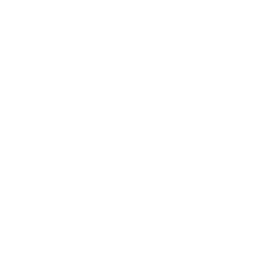
\includegraphics[scale=1]{assets/branding/opa0}
    \vspace{-5.75cm}\\
    {\adjustbox{scale=2.15}{\color{TealDarkCyan}\;III.\;Hamming Codes}}
    \bigskip\bigskip
    {\ }\vspace{4cm}\\
    \bigskip
  \end{center}
\end{frame}

%--- NEW: Historical Motivation ---
\begin{frame}{\textbf{III. Hamming Codes}}{Hamming (1950): The Original Problem}
\small
Richard Hamming worked at Bell Labs in 1947. The relay computer he used ran \textbf{punched-card jobs} overnight — and a single wrong hole would crash the job.

\medskip
\textbf{His frustration:} ``If the machine can detect an error, why can't it fix it?''

\medskip
\defbox[Hamming's insight (1950)]{
	Add \emph{redundant} parity bits so that:
	\begin{itemize}
		\item the syndrome identifies the \textbf{exact position} of the error, and
		\item \textbf{no syndrome is wasted} — each possible syndrome maps to exactly one error pattern.
	\end{itemize}
}

\medskip
This requires $n + 1 = 2^r$ syndromes for $n$ positions, giving $n = 2^r - 1$.
%\begin{columns}[T,onlytextwidth]
%  \begin{column}{.54\textwidth}
%    Richard Hamming worked at Bell Labs in 1947. The relay computer he used ran \textbf{punched-card jobs} overnight — and a single wrong hole would crash the job.
%
%    \medskip
%    \textbf{His frustration:} ``If the machine can detect an error, why can't it fix it?''
%
%    \medskip
%    \defbox[Hamming's insight (1950)]{
%    Add \emph{redundant} parity bits so that:
%    \begin{itemize}
%      \item the syndrome identifies the \textbf{exact position} of the error, and
%      \item \textbf{no syndrome is wasted} — each possible syndrome maps to exactly one error pattern.
%    \end{itemize}
%    }
%
%    \medskip
%    This requires $n + 1 = 2^r$ syndromes for $n$ positions, giving $n = 2^r - 1$.
%  \end{column}
%  \begin{column}{.43\textwidth}
%    \begin{tikzpicture}[scale=0.88]
%      % Show how syndromes map to errors
%      \node[font=\small\bfseries, TealDarkCyan] at (1.5,4.0)
%        {Syndrome $\to$ action};
%      \draw[TealDarkCyan, thick] (0,3.6)--(3.0,3.6);
%
%      % No error
%      \node[draw=TealDarkCyan!40, rounded corners=3pt, fill=TealDarkCyan!8,
%            minimum width=2.8cm, minimum height=0.38cm, font=\scriptsize]
%        at (1.5,3.25) {$000$ $\to$ no error};
%      % Errors at positions
%      \foreach \i/\bits in {1/001, 2/010, 3/011, 4/100, 5/101, 6/110, 7/111} {
%        \pgfmathsetmacro{\yy}{3.25 - \i*0.42}
%        \node[draw=AccentCyan!60, rounded corners=3pt, fill=AccentCyan!10,
%              minimum width=2.8cm, minimum height=0.38cm, font=\scriptsize]
%          at (1.5,\yy) {$\bits$ $\to$ flip bit $\i$};
%      }
%    \end{tikzpicture}
%  \end{column}
%\end{columns}
\end{frame}

\begin{frame}{\textbf{III. Hamming Codes}}{The design problem}
\small
\begin{block}{Goal}
Construct binary linear codes that correct exactly one error and use all possible syndromes.
\end{block}
\begin{itemize}
  \item A received word has either no error or one error in position $i$.
  \item Thus there are $1+n$ elementary cases.
  \item With $r$ parity checks, there are $2^r$ syndromes.
\end{itemize}
\[
  1+n=2^r
  \quad\Rightarrow\quad
  n=2^r-1.
\]
\end{frame}

\begin{frame}{\textbf{III. Hamming Codes}}{The parity-check matrix}
\small
\defbox[Binary Hamming matrix]{
For $r\ge2$, let $H_r$ be the $r\times(2^r-1)$ matrix whose columns are all nonzero vectors of $\F_2^r$.
}
\[
  H_3=
  \begin{bmatrix}
  1&0&1&0&1&0&1\\
  0&1&1&0&0&1&1\\
  0&0&0&1&1&1&1
  \end{bmatrix}.
\]
\begin{itemize}
  \item Column labels are nonzero binary syndromes.
  \item Every nonzero syndrome identifies a unique column.
\end{itemize}
\end{frame}

\begin{frame}{\textbf{III. Hamming Codes}}{Definition}
\small
\defbox[Binary Hamming code]{
The binary Hamming code of order $r$ is
\[
  \operatorname{Ham}(r,2)=\ker(H_r)\le\F_2^{2^r-1}.
\]
}
\begin{itemize}
  \item Length: $n=2^r-1$.
  \item Redundancy: $r$.
  \item Dimension: $k=n-r=2^r-1-r$.
\end{itemize}
\[
  \operatorname{Ham}(r,2)\text{ has parameters }[2^r-1,2^r-1-r,3]_2.
\]
\end{frame}

\begin{frame}{\textbf{III. Hamming Codes}}{Dimension}
\small
\thmbox[Dimension count]{
The matrix $H_r$ has rank $r$, hence
\[
  \dim\ker(H_r)=2^r-1-r.
\]
}
%\begin{proof}
%The standard basis vectors $e_1,\ldots,e_r$ occur among the nonzero columns of $H_r$, so the row rank is $r$.
%\end{proof}
%\begin{block}{Interpretation}
%The parity checks are independent; no check is redundant.
%\end{block}
\end{frame}

\begin{frame}{\textbf{III. Hamming Codes}}{Minimum distance}
\small
\thmbox[Distance]{
The binary Hamming code $\operatorname{Ham}(r,2)$ has minimum distance $3$.
}
%\begin{proof}
%No column of $H_r$ is zero, so $d\ge2$. No two columns are equal over $\F_2$, so no two are dependent, hence $d\ge3$. But $u+v+(u+v)=0$, so three suitable columns are dependent.
%\end{proof}
\begin{itemize}
  \item Therefore Hamming codes correct one error.
  \item They detect two errors.
\end{itemize}
\end{frame}

\begin{frame}{\textbf{III. Hamming Codes}}{Perfectness}
\small
\thmbox[Hamming codes are perfect]{
The binary Hamming code satisfies equality in the Hamming bound for $t=1$.
}
\[
  2^k(1+n)=2^{2^r-1-r}(1+2^r-1)=2^{2^r-1}=2^n.
\]
\begin{itemize}
  \item Every word of $\F_2^n$ is at distance at most $1$ from exactly one codeword.
  \item The syndrome is not merely a diagnostic: it is a complete decoder.
\end{itemize}
\end{frame}

%--- NEW: Perfect Tiling Visual ---
\begin{frame}{\textbf{III. Hamming Codes}}{Perfect Tiling: A Geometric View}
\small
\begin{columns}[T,onlytextwidth]
  \begin{column}{.48\textwidth}
    For the $[3,1,3]$ repetition code in $\F_2^3$: the two correction balls of radius 1 \textbf{tile the cube exactly} — no overlap, no gap.

    \medskip
    \begin{center}
    \begin{tikzpicture}[scale=0.80]
      % 3-cube edges
      \draw[gray!35,thick] (0,0)--(2,0); \draw[gray!35,thick] (0,0)--(1,0.9);
      \draw[gray!35,thick] (0,0)--(0.5,1.6); \draw[gray!35,thick] (2,0)--(3,0.9);
      \draw[gray!35,thick] (2,0)--(2.5,1.6); \draw[gray!35,thick] (1,0.9)--(3,0.9);
      \draw[gray!35,thick] (1,0.9)--(1.5,2.5); \draw[gray!35,thick] (0.5,1.6)--(2.5,1.6);
      \draw[gray!35,thick] (0.5,1.6)--(1.5,2.5); \draw[gray!35,thick] (3,0.9)--(3.5,2.5);
      \draw[gray!35,thick] (2.5,1.6)--(3.5,2.5); \draw[gray!35,thick] (1.5,2.5)--(3.5,2.5);
      % Ball around 000: {000,100,010,001} — TealDarkCyan fill
      \node[circle,draw=TealDarkCyan,fill=TealDarkCyan!20,minimum size=0.62cm,font=\tiny\bfseries]
        at (0,0)     {$000$};
      \node[circle,draw=TealDarkCyan,fill=TealDarkCyan!20,minimum size=0.62cm,font=\tiny\bfseries]
        at (2,0)     {$100$};
      \node[circle,draw=TealDarkCyan,fill=TealDarkCyan!20,minimum size=0.62cm,font=\tiny\bfseries]
        at (1,0.9)   {$010$};
      \node[circle,draw=TealDarkCyan,fill=TealDarkCyan!20,minimum size=0.62cm,font=\tiny\bfseries]
        at (0.5,1.6) {$001$};
      % Ball around 111: {111,011,101,110} — AccentCyan fill
      \node[circle,draw=AccentCyan,fill=AccentCyan!22,minimum size=0.62cm,font=\tiny\bfseries]
        at (3.5,2.5) {$111$};
      \node[circle,draw=AccentCyan,fill=AccentCyan!22,minimum size=0.62cm,font=\tiny\bfseries]
        at (1.5,2.5) {$011$};
      \node[circle,draw=AccentCyan,fill=AccentCyan!22,minimum size=0.62cm,font=\tiny\bfseries]
        at (2.5,1.6) {$101$};
      \node[circle,draw=AccentCyan,fill=AccentCyan!22,minimum size=0.62cm,font=\tiny\bfseries]
        at (3,0.9)   {$110$};
      % Codeword labels
      \node[below=3pt,font=\tiny,TealDarkCyan] at (0,0)     {\textbf{c=000}};
      \node[above=3pt,font=\tiny,AccentCyan]   at (3.5,2.5) {\textbf{c=111}};
    \end{tikzpicture}
	\end{center}
  \end{column}
  \begin{column}{.49\textwidth}
    \textcolor{TealDarkCyan}{\textbf{Why "perfect"?}}
    \begin{itemize}
      \item Each ball has 4 elements: 1 codeword + 3 neighbors
      \item Two balls cover all $2^3 = 8$ points of $\F_2^3$
      \item $2 \times 4 = 8$ — the Hamming bound holds with \emph{equality}
    \end{itemize}

%    \medskip
%    \defbox[For $\operatorname{Ham}(r,2)$]{
%    $2^{2^r-1-r} \times (1 + 2^r - 1) = 2^{2^r-1}$ — all of $\F_2^{2^r-1}$ is tiled.\\[2pt]
%    Every received word is within distance 1 of \textbf{exactly one} codeword.
%    }

    \medskip
    Hamming codes are the \emph{only} linear perfect 1-error-correcting codes (apart from trivial cases).
  \end{column}
\end{columns}
\end{frame}

\begin{frame}{\textbf{III. Hamming Codes}}{Syndrome decoding}
\small
\defbox[Decoder]{
Given $v\in\F_2^n$, compute $s=H_rv^T$.
}
\begin{itemize}
  \item If $s=0$, accept $v$.
  \item If $s\ne0$, find the unique column $H_i=s$.
  \item Correct by flipping coordinate $i$.
\end{itemize}
%\begin{block}{Reason}
%For a single error $e_i$, the syndrome is $H_re_i^T=H_i$.
%\end{block}
\end{frame}

%--- NEW: Full Syndrome Decoder Table ---
\begin{frame}{\textbf{III. Hamming Codes}}{The Complete Syndrome Table for $[7,4,3]$}
\small
With $H_3$ as written, the syndrome $(s_1,s_2,s_3)^T$ equals column $i$ when bit $i$ is flipped.

\medskip
\begin{center}
\begin{tikzpicture}[scale=0.82]
  % Header
  \node[font=\scriptsize\bfseries,TealDarkCyan] at (0.0,3.5) {Syndrome %$(s_1\,s_2\,s_3)$
  };
  \node[font=\scriptsize\bfseries,TealDarkCyan] at (2.5,3.5) {Error pattern $e$};
  \node[font=\scriptsize\bfseries,TealDarkCyan] at (5.2,3.5) {Action};
  \draw[TealDarkCyan!50,thick] (-0.8,3.25)--(6.0,3.25);
  % Row 0: no error
  \node[draw=TealDarkCyan!30,fill=TealDarkCyan!8,rounded corners=2pt,
        minimum width=2.0cm,minimum height=0.34cm,font=\scriptsize]
    at (0.0,3.0) {$(0,0,0)$};
  \node[font=\scriptsize] at (2.5,3.0) {$0000000$};
  \node[font=\scriptsize,TealDarkCyan] at (5.2,3.0) {no error — accept};
  % Rows 1-7: each error position
  \node[draw=AccentCyan,fill=AccentCyan!12,rounded corners=2pt,
        minimum width=2.0cm,minimum height=0.34cm,font=\scriptsize]
    at (0.0,2.6) {$(1,0,0)$};
  \node[font=\scriptsize] at (2.5,2.6) {$1000000$};
  \node[font=\scriptsize,AccentCyan] at (5.2,2.6) {flip bit 1};

  \node[draw=AccentCyan,fill=AccentCyan!12,rounded corners=2pt,
        minimum width=2.0cm,minimum height=0.34cm,font=\scriptsize]
    at (0.0,2.2) {$(0,1,0)$};
  \node[font=\scriptsize] at (2.5,2.2) {$0100000$};
  \node[font=\scriptsize,AccentCyan] at (5.2,2.2) {flip bit 2};

  \node[draw=AccentCyan,fill=AccentCyan!12,rounded corners=2pt,
        minimum width=2.0cm,minimum height=0.34cm,font=\scriptsize]
    at (0.0,1.8) {$(1,1,0)$};
  \node[font=\scriptsize] at (2.5,1.8) {$0010000$};
  \node[font=\scriptsize,AccentCyan] at (5.2,1.8) {flip bit 3};

  \node[draw=AccentCyan,fill=AccentCyan!12,rounded corners=2pt,
        minimum width=2.0cm,minimum height=0.34cm,font=\scriptsize]
    at (0.0,1.4) {$(0,0,1)$};
  \node[font=\scriptsize] at (2.5,1.4) {$0001000$};
  \node[font=\scriptsize,AccentCyan] at (5.2,1.4) {flip bit 4};

  \node[draw=AccentCyan,fill=AccentCyan!12,rounded corners=2pt,
        minimum width=2.0cm,minimum height=0.34cm,font=\scriptsize]
    at (0.0,1.0) {$(1,0,1)$};
  \node[font=\scriptsize] at (2.5,1.0) {$0000100$};
  \node[font=\scriptsize,AccentCyan] at (5.2,1.0) {flip bit 5};

  \node[draw=AccentCyan,fill=AccentCyan!12,rounded corners=2pt,
        minimum width=2.0cm,minimum height=0.34cm,font=\scriptsize]
    at (0.0,0.6) {$(0,1,1)$};
  \node[font=\scriptsize] at (2.5,0.6) {$0000010$};
  \node[font=\scriptsize,AccentCyan] at (5.2,0.6) {flip bit 6};

  \node[draw=AccentCyan,fill=AccentCyan!12,rounded corners=2pt,
        minimum width=2.0cm,minimum height=0.34cm,font=\scriptsize]
    at (0.0,0.2) {$(1,1,1)$};
  \node[font=\scriptsize] at (2.5,0.2) {$0000001$};
  \node[font=\scriptsize,AccentCyan] at (5.2,0.2) {flip bit 7};
\end{tikzpicture}
\end{center}

\vspace{-2pt}
\begin{itemize}
  \item All $2^3 = 8$ syndromes are used — confirming \textbf{perfectness}
  \item Decoding is a single table look-up — $O(1)$ hardware
\end{itemize}
\end{frame}

\begin{frame}{\textbf{III. Hamming Codes}}{Binary index convention}
\small
\defbox[Indexed columns]{
If the $i$-th column of $H_r$ is the binary expansion of $i$, then the nonzero syndrome is literally the error position.
}
\[
  s=(1,0,1)^T\quad\leadsto\quad i=5
\]
depending on the chosen bit order.
\begin{itemize}
  \item This is a notational convention, not an invariant.
  \item It explains the classical parity-bit positions $1,2,4,\ldots$.
\end{itemize}
\end{frame}

\begin{frame}{\textbf{III. Hamming Codes}}{The classical [7,4,3] code}
\small
\[
H=
\begin{bmatrix}
1&0&1&0&1&0&1\\
0&1&1&0&0&1&1\\
0&0&0&1&1&1&1
\end{bmatrix}.
\]
\begin{itemize}
  \item There are $7$ nonzero syndromes.
  \item Each syndrome names one error coordinate.
  \item The kernel has dimension $4$.
\end{itemize}
\[
  \operatorname{Ham}(3,2)=[7,4,3]_2.
\]
\end{frame}

%--- NEW: Parity Bit Layout ---
\begin{frame}{\textbf{III. Hamming Codes}}{The $[7,4,3]$ Code: Parity Bit Positions}
\small
Bits are numbered $1$ through $7$. Positions that are powers of 2 ($1, 2, 4$) are \textcolor{AccentCyan}{\textbf{parity bits}}; the rest carry \textcolor{TealDarkCyan}{\textbf{data}}.

\medskip
\begin{center}
\begin{tikzpicture}[scale=0.88]
  % Seven position boxes
  \foreach \i/\type in {1/par, 2/par, 3/data, 4/par, 5/data, 6/data, 7/data} {
    \pgfmathsetmacro{\xp}{(\i-1)*1.05}
    \ifnum\i=1
      \node[draw=AccentCyan, thick, fill=AccentCyan!20, rounded corners=4pt,
            minimum width=0.9cm, minimum height=0.9cm, font=\small\bfseries]
        (b\i) at (\xp,0) {$p_1$};
    \else\ifnum\i=2
      \node[draw=AccentCyan, thick, fill=AccentCyan!20, rounded corners=4pt,
            minimum width=0.9cm, minimum height=0.9cm, font=\small\bfseries]
        (b\i) at (\xp,0) {$p_2$};
    \else\ifnum\i=4
      \node[draw=AccentCyan, thick, fill=AccentCyan!20, rounded corners=4pt,
            minimum width=0.9cm, minimum height=0.9cm, font=\small\bfseries]
        (b\i) at (\xp,0) {$p_4$};
    \else
      \node[draw=TealDarkCyan, thick, fill=TealDarkCyan!12, rounded corners=4pt,
            minimum width=0.9cm, minimum height=0.9cm, font=\small\bfseries]
        (b\i) at (\xp,0) {$d_{\i}$};
    \fi\fi\fi
    \node[font=\tiny, TealDarkCyan!70] at (\xp,-0.62) {bit \i};
  }
\end{tikzpicture}
\end{center}

\medskip
\textbf{Parity check coverage:}
\begin{center}
\begin{tabular}{c|l|l}
  \textbf{Parity bit} & \textbf{Checks bits} & \textbf{Syndrome row} \\\hline
  $p_1$ (bit 1) & 1, 3, 5, 7 & $H$ row 1: $(1,0,1,0,1,0,1)$ \\
  $p_2$ (bit 2) & 2, 3, 6, 7 & $H$ row 2: $(0,1,1,0,0,1,1)$ \\
  $p_4$ (bit 4) & 4, 5, 6, 7 & $H$ row 3: $(0,0,0,1,1,1,1)$ \\
\end{tabular}
\end{center}

\medskip
\begin{itemize}
  \item Each parity bit checks all positions whose index has a $1$ in the corresponding binary place
  \item The 3-bit syndrome tells us the \emph{binary address} of the flipped bit
\end{itemize}
\end{frame}

\begin{frame}{\textbf{III. Hamming Codes}}{A systematic generator matrix}
\small
One systematic form for the $[7,4,3]$ Hamming code is
\[
G=
\begin{bmatrix}
1&0&0&0&0&1&1\\
0&1&0&0&1&0&1\\
0&0&1&0&1&1&0\\
0&0&0&1&1&1&1
\end{bmatrix}.
\]
\begin{itemize}
  \item The first four coordinates are message symbols.
  \item The last three are parity symbols.
  \item This $G$ is equivalent to the kernel of a suitable $H$.
\end{itemize}
\end{frame}

\begin{frame}{\textbf{III. Hamming Codes}}{Encoding example}
\small
For $m=(1,0,1,1)$ and the systematic matrix $G$,
\[
  c=mG=(1,0,1,1,0,0,1).
\]
\begin{itemize}
  \item The parity bits are linear forms in the message bits.
  \item A single flipped bit changes the syndrome to the corresponding column.
  \item The correction rule does not require knowing the transmitted message.
\end{itemize}
\end{frame}

%--- NEW: Encoding and Error Correction Flow ---
\begin{frame}{\textbf{III. Hamming Codes}}{Encoding \& Error Correction}
\small
\begin{center}
\begin{tikzpicture}[
  box/.style={draw=TealDarkCyan,thick,rounded corners=4pt,
              minimum width=2.0cm,minimum height=0.65cm,
              fill=TealDarkCyan!10,font=\scriptsize,align=center},
  arr/.style={-Stealth,thick,TealDarkCyan},
  earr/.style={-Stealth,thick,AccentCyan,dashed}
]
  % Nodes
  \node[box] (msg)  at (0,0)   {Message\\$m=(1,0,1,1)$};
  \node[box] (enc)  at (3,0)   {Encoder\\$c=mG$};
  \node[box] (cw)   at (6,0)   {Codeword\\$c=(1,0,1,1,0,1,0)$};
  \node[box,fill=AccentCyan!12,draw=AccentCyan] (ch) at (9,0)
    {Channel\\flip bit 5};
  \node[box,fill=AccentCyan!8,draw=AccentCyan]  (rv)  at (9,-1.5)
    {Received\\$v=(1,0,1,1,\mathbf{1},1,0)$};
  \node[box] (syn)  at (6,-1.5) {Syndrome\\$s=Hv^T=(1,0,1)^T$};
  \node[box] (lkp)  at (3,-1.5) {Look up:\\col 5 of $H$};
  \node[box] (fix)  at (0,-1.5) {Correct:\\$\hat{c}=c$\;\checkmark};
  % Arrows
  \draw[arr]  (msg)--(enc);
  \draw[arr]  (enc)--(cw);
  \draw[arr]  (cw)--(ch);
  \draw[earr] (ch)--(rv);
  \draw[arr]  (rv)--(syn);
  \draw[arr]  (syn)--(lkp);
  \draw[arr]  (lkp)--(fix);
  % Labels
  \node[above=2pt,font=\tiny,TealDarkCyan] at (1.5,0)   {$mG$};
  \node[above=2pt,font=\tiny,AccentCyan]   at (9,-0.75) {noise};
  \node[above=2pt,font=\tiny,TealDarkCyan] at (7.5,-1.5) {$Hv^T$};
\end{tikzpicture}
\end{center}

\begin{columns}[T,onlytextwidth]
  \begin{column}{.50\textwidth}
    \textbf{Key numbers:}
    \begin{itemize}
      \item Syndrome $s=(1,0,1)^T$ matches column 5 of $H_3$
      \item Flip bit 5: $(1,0,1,1,\mathbf{1},1,0)\to(1,0,1,1,0,1,0)$
      \item Recovered $\hat{c}$ is the original codeword (v)
    \end{itemize}
  \end{column}
  \begin{column}{.47\textwidth}
%    \begin{block}{The decoder never needs $m$}
	The decoder never needs $m$\\
    The syndrome alone identifies the error. Once we flip the right bit, the first 4 bits of the corrected $\hat{c}$ directly give $\hat{m}=(1,0,1,1)$.
%    \end{block}
  \end{column}
\end{columns}
\end{frame}

\begin{frame}{\textbf{III. Hamming Codes}}{Projective geometry}
\small
\defbox[Projective interpretation]{
The nonzero columns of $H_r$, modulo scalar multiplication, are the points of projective space
\[
  \mathbb{P}^{r-1}(\F_q).
\]
}
\begin{itemize}
  \item Over $\F_2$, each nonzero vector is its own projective point.
  \item Over $\F_q$, scalar multiples define the same projective point.
  \item Hamming codes are parity checks indexed by projective points.
\end{itemize}
\end{frame}

\begin{frame}{\textbf{III. Hamming Codes}}{The Fano plane}
\small
For $r=3$, the projective space $\mathbb{P}^2(\F_2)$ has $7$ points and $7$ lines.
\begin{itemize}
  \item The $7$ columns of $H_3$ are the points.
  \item A dependent triple of columns is a line of the Fano plane.
  \item Weight-$3$ codewords are exactly these lines.
\end{itemize}
%\begin{block}{Geometry}
The minimum distance $3$ is the statement that the smallest projective line has three points.
%\end{block}
\end{frame}

%--- NEW: Fano Plane Drawing ---
\begin{frame}{\textbf{III. Hamming Codes}}{The Fano Plane — Drawn}
\small
\begin{columns}[T,onlytextwidth]
  \begin{column}{.44\textwidth}
    \begin{center}
    \begin{tikzpicture}[scale=0.88]
      % Outer triangle edges (3 lines of the Fano plane)
      % Line {1,2,3}: P1(0,2) -- P3(-0.865,0.5) -- P2(-1.73,-1)
      \draw[TealDarkCyan, thick] (0,2) -- (-1.73,-1);
      % Line {1,4,5}: P1(0,2) -- P5(0.865,0.5) -- P4(1.73,-1)
      \draw[TealDarkCyan, thick] (0,2) -- (1.73,-1);
      % Line {2,4,6}: P2(-1.73,-1) -- P6(0,-1) -- P4(1.73,-1)
      \draw[TealDarkCyan, thick] (-1.73,-1) -- (1.73,-1);
      % Three "altitude" lines (through center P7=(0,0))
      % Line {1,7,6}: P1(0,2) -- P7(0,0) -- P6(0,-1)
      \draw[AccentCyan, thick] (0,2) -- (0,-1);
      % Line {2,7,5}: P2(-1.73,-1) -- P7(0,0) -- P5(0.865,0.5)
      \draw[AccentCyan, thick] (-1.73,-1) -- (0.865,0.5);
      % Line {3,7,4}: P3(-0.865,0.5) -- P7(0,0) -- P4(1.73,-1)
      \draw[AccentCyan, thick] (-0.865,0.5) -- (1.73,-1);
      % Inner circle through {3,5,6} (circumradius ≈ 1 centered at P7=(0,0))
      \draw[TealDarkCyan!55, thick] (0,0) circle (1.0);
      % Points — outer triangle (columns 1,2,4)
      \fill[TealDarkCyan] (0,2)      circle (3.5pt);
      \node[above=3pt, font=\scriptsize, TealDarkCyan]
        at (0,2)      {$1\ (100)$};
      \fill[TealDarkCyan] (-1.73,-1) circle (3.5pt);
      \node[left=3pt,  font=\scriptsize, TealDarkCyan]
        at (-1.73,-1) {$2\ (010)$};
      \fill[TealDarkCyan] (1.73,-1)  circle (3.5pt);
      \node[right=3pt, font=\scriptsize, TealDarkCyan]
        at (1.73,-1)  {$4\ (001)$};
      % Edge midpoints (columns 3,5,6)
      \fill[AccentCyan] (-0.865,0.5) circle (3.5pt);
      \node[left=3pt,  font=\scriptsize, AccentCyan]
        at (-0.865,0.5) {$3\ (110)$};
      \fill[AccentCyan] (0.865,0.5)  circle (3.5pt);
      \node[right=3pt, font=\scriptsize, AccentCyan]
        at (0.865,0.5)  {$5\ (101)$};
      \fill[AccentCyan] (0,-1)        circle (3.5pt);
      \node[below=3pt, font=\scriptsize, AccentCyan]
        at (0,-1)       {$6\ (011)$};
      % Center (column 7)
      \fill[TealDarkCyan!70] (0,0) circle (3.5pt);
      \node[right=4pt, font=\scriptsize, TealDarkCyan]
        at (0,0) {$7\ (111)$};
    \end{tikzpicture}
    \end{center}
  \end{column}
  \begin{column}{.53\textwidth}
    \textcolor{TealDarkCyan}{\textbf{The 7 lines (each has 3 points):}}
    \smallskip

    \begin{tabular}{c|l|l}
      \# & \textbf{Points} & \textbf{Columns sum to 0} \\\hline
      \rowcolor{TealDarkCyan!8}
      1 & $\{1,2,3\}$ & $100{+}010{=}110$ \\
      2 & $\{1,4,5\}$ & $100{+}001{=}101$ \\
      \rowcolor{TealDarkCyan!8}
      3 & $\{2,4,6\}$ & $010{+}001{=}011$ \\
      4 & $\{1,6,7\}$ & $100{+}011{=}111$ \\
      \rowcolor{TealDarkCyan!8}
      5 & $\{2,5,7\}$ & $010{+}101{=}111$ \\
      6 & $\{3,4,7\}$ & $110{+}001{=}111$ \\
      \rowcolor{TealDarkCyan!8}
      7 & $\{3,5,6\}$ & $110{+}101{=}011$ \\
    \end{tabular}

%    \bigskip
%    \begin{block}{Why minimum distance $= 3$}
%    Each line is a weight-$3$ codeword. No point lies alone (weight-$1$), no pair sums to zero (weight-$2$). Hence $d = 3$.
%    \end{block}
  \end{column}
\end{columns}
\end{frame}

\begin{frame}{\textbf{III. Hamming Codes}}{Lines give codewords}
\small
In $\mathbb{P}^2(\F_2)$, if $a,b,c$ are the three points on a line, then
\[
  a+b+c=0.
\]
\begin{itemize}
  \item The incidence vector of that line is a Hamming codeword.
  \item The $7$ lines give the $7$ words of weight $3$.
  \item Their complements give $7$ words of weight $4$.
\end{itemize}
\[
  W_{\operatorname{Ham}(3,2)}(Y)=1+7Y^3+7Y^4+Y^7.
\]
\end{frame}

\begin{frame}{\textbf{III. Hamming Codes}}{The simplex dual}
\small
\defbox[Simplex code]{
The row space of $H_r$ is the binary simplex code:
\[
  \operatorname{Sim}(r,2)=\operatorname{rowspan}(H_r).
\]
}
\begin{itemize}
  \item It has parameters $[2^r-1,r,2^{r-1}]_2$.
  \item Every nonzero word has weight $2^{r-1}$.
  \item It is dual to the Hamming code.
\end{itemize}
\[
  \operatorname{Ham}(r,2)^\perp=\operatorname{Sim}(r,2).
\]
\end{frame}

\begin{frame}{\textbf{III. Hamming Codes}}{MacWilliams check}
\small
For $r=3$, the simplex code has weight enumerator
\[
  W_{\operatorname{Sim}}(X,Y)=X^7+7X^3Y^4.
\]
Applying MacWilliams gives
\[
  W_{\operatorname{Ham}}(X,Y)=X^7+7X^4Y^3+7X^3Y^4+Y^7.
\]
\begin{itemize}
  \item The algebraic transform recovers the geometric weight distribution.
  \item Duality is visible both in matrices and in enumerators.
\end{itemize}
\end{frame}

\begin{frame}{\textbf{III. Hamming Codes}}{Q-ary Hamming codes}
\small
\defbox[Q-ary construction]{
Choose one nonzero representative from each one-dimensional subspace of $\F_q^r$ and use these vectors as columns of $H$.
}
\[
  n=\frac{q^r-1}{q-1}.
\]
\begin{itemize}
  \item The resulting code has parameters
  \[
    \left[\frac{q^r-1}{q-1},\frac{q^r-1}{q-1}-r,3\right]_q.
  \]
  \item It is again perfect for one-error correction.
\end{itemize}
\end{frame}

\begin{frame}{\textbf{III. Hamming Codes}}{Why projective representatives}
\small
Over $\F_q$, two proportional nonzero columns are linearly dependent.
\begin{itemize}
  \item To have $d\ge3$, no two columns may be proportional.
  \item Therefore columns must be projective points, not raw nonzero vectors.
  \item Taking all projective points uses the maximum possible number of columns.
\end{itemize}
%\begin{block}{Conclusion}
Hamming codes are the maximal parity-check configurations with no zero column and no repeated projective point.
%\end{block}
\end{frame}

\begin{frame}{\textbf{III. Hamming Codes}}{Q-ary perfectness}
\small
For the $q$-ary Hamming code,
\[
  n=\frac{q^r-1}{q-1},\qquad k=n-r.
\]
The radius-one sphere has size
\[
  1+n(q-1)=1+q^r-1=q^r.
\]
Hence
\[
  q^k(1+n(q-1))=q^{n-r}q^r=q^n.
\]
%\begin{block}{Perfect again}
Every received word lies at distance at most one from a unique codeword.
%\end{block}
\end{frame}

%%--- NEW: Hamming Family Parameters ---
%\begin{frame}{\textbf{III. Hamming Codes}}{The Hamming Family: Parameters at a Glance}
%\small
%\begin{center}
%\begin{tikzpicture}[scale=0.88]
%  % Table header
%  \node[font=\scriptsize\bfseries,TealDarkCyan] at (0.0,4.5) {$r$};
%  \node[font=\scriptsize\bfseries,TealDarkCyan] at (1.2,4.5) {$n=2^r{-}1$};
%  \node[font=\scriptsize\bfseries,TealDarkCyan] at (2.6,4.5) {$k=n{-}r$};
%  \node[font=\scriptsize\bfseries,TealDarkCyan] at (3.9,4.5) {Rate $k/n$};
%  \node[font=\scriptsize\bfseries,TealDarkCyan] at (5.3,4.5) {$t$ corrected};
%  \node[font=\scriptsize\bfseries,TealDarkCyan] at (6.7,4.5) {Use case};
%  \draw[TealDarkCyan!40,thick] (-0.4,4.25)--(7.5,4.25);
%  % r=2
%  \node[font=\scriptsize] at (0.0,3.9) {2};
%  \node[font=\scriptsize] at (1.2,3.9) {3};
%  \node[font=\scriptsize] at (2.6,3.9) {1};
%  \node[font=\scriptsize] at (3.9,3.9) {$33\%$};
%  \node[font=\scriptsize] at (5.3,3.9) {1};
%  \node[font=\scriptsize,gray] at (6.7,3.9) {tiny};
%  % r=3
%  \node[draw=TealDarkCyan!30,fill=TealDarkCyan!8,rounded corners=2pt,
%        minimum width=6.6cm,minimum height=0.34cm] at (3.35,3.45) {};
%  \node[font=\scriptsize\bfseries,TealDarkCyan] at (0.0,3.45) {3};
%  \node[font=\scriptsize\bfseries,TealDarkCyan] at (1.2,3.45) {7};
%  \node[font=\scriptsize\bfseries,TealDarkCyan] at (2.6,3.45) {4};
%  \node[font=\scriptsize\bfseries,TealDarkCyan] at (3.9,3.45) {$57\%$};
%  \node[font=\scriptsize\bfseries,TealDarkCyan] at (5.3,3.45) {1};
%  \node[font=\scriptsize\bfseries,TealDarkCyan] at (6.7,3.45) {[7,4,3]};
%  % r=4
%  \node[font=\scriptsize] at (0.0,3.0) {4};
%  \node[font=\scriptsize] at (1.2,3.0) {15};
%  \node[font=\scriptsize] at (2.6,3.0) {11};
%  \node[font=\scriptsize] at (3.9,3.0) {$73\%$};
%  \node[font=\scriptsize] at (5.3,3.0) {1};
%  \node[font=\scriptsize,gray] at (6.7,3.0) {medium};
%  % r=5
%  \node[draw=TealDarkCyan!30,fill=TealDarkCyan!8,rounded corners=2pt,
%        minimum width=6.6cm,minimum height=0.34cm] at (3.35,2.55) {};
%  \node[font=\scriptsize] at (0.0,2.55) {5};
%  \node[font=\scriptsize] at (1.2,2.55) {31};
%  \node[font=\scriptsize] at (2.6,2.55) {26};
%  \node[font=\scriptsize] at (3.9,2.55) {$84\%$};
%  \node[font=\scriptsize] at (5.3,2.55) {1};
%  \node[font=\scriptsize,gray] at (6.7,2.55) {medium};
%  % r=6
%  \node[font=\scriptsize] at (0.0,2.1) {6};
%  \node[font=\scriptsize] at (1.2,2.1) {63};
%  \node[font=\scriptsize] at (2.6,2.1) {57};
%  \node[font=\scriptsize] at (3.9,2.1) {$90\%$};
%  \node[font=\scriptsize] at (5.3,2.1) {1};
%  \node[font=\scriptsize,gray] at (6.7,2.1) {large};
%  % r=8 (ECC RAM extended)
%  \node[draw=AccentCyan!20,fill=AccentCyan!8,rounded corners=2pt,
%        minimum width=6.6cm,minimum height=0.34cm] at (3.35,1.65) {};
%  \node[font=\scriptsize,AccentCyan] at (0.0,1.65) {$*$};
%  \node[font=\scriptsize\bfseries,AccentCyan] at (1.2,1.65) {72};
%  \node[font=\scriptsize\bfseries,AccentCyan] at (2.6,1.65) {64};
%  \node[font=\scriptsize\bfseries,AccentCyan] at (3.9,1.65) {$89\%$};
%  \node[font=\scriptsize\bfseries,AccentCyan] at (5.3,1.65) {1 (SECDED)};
%  \node[font=\scriptsize\bfseries,AccentCyan] at (6.7,1.65) {ECC RAM};
%\end{tikzpicture}
%\end{center}
%
%\vspace{-4pt}
%{\footnotesize $*$ Extended Hamming code $[72,64,4]_2$: shortened and extended for byte-aligned memory.}
%
%\begin{itemize}
%  \item Rate $\to 1$ as $r \to \infty$ — Hamming codes become increasingly efficient
%  \item All correct exactly \textbf{one} bit error (single-error-correcting)
%\end{itemize}
%\end{frame}

\begin{frame}{\textbf{III. Hamming Codes}}{Extended Hamming codes}
\small
\defbox[Extension]{
Add one overall parity coordinate to force even total weight.
}
\begin{itemize}
  \item The binary $[7,4,3]$ code becomes an $[8,4,4]$ code.
  \item The new minimum distance is $4$.
  \item It detects three errors and corrects one error.
\end{itemize}
\[
  \widehat{\operatorname{Ham}}(3,2)=[8,4,4]_2.
\]
\end{frame}

\begin{frame}{\textbf{III. Hamming Codes}}{The [8,4,4] code}
\small
The extended Hamming code has weight enumerator
\[
  W(X,Y)=X^8+14X^4Y^4+Y^8.
\]
\begin{itemize}
  \item All codeword weights are divisible by $4$.
  \item The code is self-dual.
  \item It is the smallest doubly-even self-dual binary code.
\end{itemize}
%\begin{block}{Connection}
This code is the length-$8$ seed behind the $E_8$ lattice construction.
%\end{block}
\end{frame}

\begin{frame}{\textbf{III. Hamming Codes}}{Automorphisms}
\small
\defbox[Symmetry group]{
The automorphism group of the binary Hamming code is induced by invertible linear transformations of $\F_2^r$:
\[
  \Aut(\operatorname{Ham}(r,2))\cong \operatorname{GL}(r,2).
\]
}
\begin{itemize}
  \item A matrix in $\operatorname{GL}(r,2)$ permutes the nonzero columns of $H_r$.
  \item Hence it permutes coordinates and preserves the kernel.
  \item The code remembers the projective geometry.
\end{itemize}
\end{frame}

\begin{frame}{\textbf{III. Hamming Codes}}{Tanner graph}
\small
\begin{itemize}
  \item The Tanner graph of $H_r$ has $n=2^r-1$ variable nodes and $r$ check nodes.
  \item It is dense compared with modern LDPC codes.
  \item But it has an exceptionally simple exact decoder.
\end{itemize}
\begin{block}{Interpretation}
For Hamming codes, the syndrome is not iteratively refined; it is read directly as a projective point.
\end{block}
\end{frame}

\begin{frame}{\textbf{III. Hamming Codes}}{Failure modes}
\small
\begin{itemize}
  \item A two-error pattern has syndrome equal to the sum of two columns.
  \item In a binary Hamming matrix, that sum is another nonzero column.
  \item Therefore a two-error pattern may be miscorrected as a one-error pattern.
\end{itemize}
%\begin{block}{Moral}
Minimum distance $3$ guarantees single-error correction, not reliable detection after attempting correction.
%\end{block}
\end{frame}

%\begin{frame}{\textbf{III. Hamming Codes}}{SECDED}
%\small
%\defbox[SECDED]{
%Single-error correction, double-error detection is obtained by using the extended Hamming code.
%}
%\begin{itemize}
%  \item The extension raises the distance from $3$ to $4$.
%  \item One error is corrected by the Hamming syndrome.
%  \item Two errors are detected because parity and syndrome disagree in a recognizable way.
%\end{itemize}
%\end{frame}
%
%%--- NEW: ECC RAM Application ---
%\begin{frame}{\textbf{III. Hamming Codes}}{ECC Memory: Hamming in Your Computer}
%\small
%\begin{columns}[T,onlytextwidth]
%  \begin{column}{.54\textwidth}
%    \textcolor{TealDarkCyan}{\textbf{Error-correcting DRAM (ECC RAM)}}
%
%    \medskip
%    Standard server RAM uses the \textbf{extended Hamming code $[72, 64, 4]_2$}:
%    \begin{itemize}
%      \item $64$ data bits + $8$ check bits per 64-bit memory word
%      \item Corrects \emph{any single-bit} error automatically
%      \item Detects (but does not correct) any \emph{double-bit} error
%      \item Rate $= 64/72 \approx 89\%$ — very efficient
%    \end{itemize}
%
%    \medskip
%    \textcolor{TealDarkCyan}{\textbf{Why does it matter?}}
%    \begin{itemize}
%      \item Cosmic rays and thermal noise can flip a bit in DRAM roughly once per gigabyte per day
%      \item In a server with $1\,\text{TB}$ of RAM, that is $\sim 1000$ bit flips per day
%      \item ECC corrects each flip silently — the OS never sees it
%    \end{itemize}
%  \end{column}
%  \begin{column}{.43\textwidth}
%    \begin{tikzpicture}[scale=0.82]
%      % 72-bit word as colored blocks
%      \node[font=\scriptsize\bfseries, TealDarkCyan] at (1.8,3.5) {72-bit ECC word};
%
%      % Data bits (64): draw 4 rows of 16 → simplified as 4 wide bars
%      \foreach \row in {1,2,3,4} {
%        \pgfmathsetmacro{\yy}{3.1-(\row-1)*0.45}
%        \node[draw=TealDarkCyan, fill=TealDarkCyan!15, rounded corners=2pt,
%              minimum width=3.2cm, minimum height=0.38cm, font=\tiny]
%          at (1.2,\yy) {data bits (16 each)};
%      }
%      % Check bits (8)
%      \node[draw=AccentCyan, fill=AccentCyan!22, rounded corners=2pt,
%            minimum width=3.2cm, minimum height=0.38cm, font=\tiny\bfseries]
%        at (1.2,1.25) {8 check bits (Hamming)};
%
%      % Brace
%      \draw[TealDarkCyan, decorate,
%            decoration={brace, amplitude=4pt, raise=3pt, mirror}]
%        (2.85,1.08) -- (2.85,3.30);
%      \node[right=10pt, font=\tiny, TealDarkCyan] at (2.85,2.2) {72 bits total};
%
%      \medskip
%      \node[draw=TealDarkCyan!40, rounded corners=4pt, fill=TealDarkCyan!5,
%            minimum width=3.4cm, minimum height=0.9cm, font=\scriptsize,
%            align=center] at (1.5,0.5)
%        {Syndrome = 0: OK\\Syndrome $\ne$ 0: fix bit};
%    \end{tikzpicture}
%  \end{column}
%\end{columns}
%\end{frame}
%
%\begin{frame}{\textbf{III. Hamming Codes}}{Shortened Hamming codes}
%\small
%\defbox[Shortening]{
%Shortened Hamming codes are obtained by fixing selected coordinates to zero and deleting them.
%}
%\begin{itemize}
%  \item They are useful when exact lengths $2^r-1$ are inconvenient.
%  \item The minimum distance remains at least $3$.
%  \item Perfectness is usually lost.
%\end{itemize}
%\begin{block}{Engineering}
%Many practical memory codes are shortened or extended Hamming codes.
%\end{block}
%\end{frame}

\begin{frame}{\textbf{III. Hamming Codes}}{Hamming codes as BCH codes}
\small
\defbox[Cyclic viewpoint]{
When $n=2^r-1$, the binary Hamming code can be realized as a narrow-sense BCH code of designed distance $3$.
}
\begin{itemize}
  \item Choose a primitive $n$-th root $\alpha\in\F_{2^r}$.
  \item Let $g(X)$ be the minimal polynomial of $\alpha$ over $\F_2$.
  \item Then the cyclic code generated by $g(X)$ is a Hamming code.
\end{itemize}
\end{frame}

\begin{frame}{\textbf{III. Hamming Codes}}{The [7,4,3] cyclic form}
\small
Over $\F_2$,
\[
  X^7-1=(X+1)(X^3+X+1)(X^3+X^2+1).
\]
Taking
\[
  g(X)=X^3+X+1
\]
gives a cyclic $[7,4,3]$ Hamming code.
\begin{itemize}
  \item This is the bridge from projective checks to polynomial ideals.
  \item The next chapter makes that bridge systematic.
\end{itemize}
\end{frame}

\begin{frame}{\textbf{III. Hamming Codes}}{Classification intuition}
\small
\begin{itemize}
  \item Perfect one-error-correcting linear codes are essentially Hamming codes, apart from trivial cases.
  \item The parity-check matrix must use every possible nonzero syndrome once.
  \item Thus the construction is forced by the Hamming bound.
\end{itemize}
%\begin{block}{Mathematical taste}
Hamming codes are beautiful because optimality, decoding, and geometry are the same statement.
%\end{block}
\end{frame}

%\begin{frame}{\textbf{III. Hamming Codes}}{Exercise: distance}
%\small
%\begin{block}{Problem}
%Let $H$ contain one representative of every point of $\mathbb{P}^{r-1}(\F_q)$. Prove that $\ker H$ has distance exactly $3$.
%\end{block}
%\textbf{Hint.}
%\begin{itemize}
%  \item No one or two columns are dependent.
%  \item Any projective line contains three dependent representatives after scaling.
%  \item Translate column dependence into a codeword support.
%\end{itemize}
%\end{frame}
%
%\begin{frame}{\textbf{III. Hamming Codes}}{Exercise: perfectness}
%\small
%\begin{block}{Problem}
%Verify directly that the $q$-ary Hamming code meets the Hamming bound with equality for $t=1$.
%\end{block}
%\[
%  n=\frac{q^r-1}{q-1},\qquad k=n-r.
%\]
%\textbf{Computation.}
%\[
%  q^k(1+n(q-1))=q^{n-r}(1+q^r-1)=q^n.
%\]
%\end{frame}
%
%\begin{frame}{\textbf{III. Hamming Codes}}{Exercise: dual weights}
%\small
%\begin{block}{Problem}
%Show that every nonzero word of the binary simplex code has weight $2^{r-1}$.
%\end{block}
%\textbf{Hint.}
%For a nonzero row vector $a\in\F_2^r$, the word $aH_r$ evaluates the nonzero linear functional $x\mapsto ax^T$ on every nonzero vector $x$.
%\begin{itemize}
%  \item Exactly half of all vectors of $\F_2^r$ evaluate to $1$.
%  \item The zero vector evaluates to $0$.
%\end{itemize}
%\end{frame}

\begin{frame}{\textbf{III. Hamming Codes}}{Summary}
\small
\begin{columns}[T,onlytextwidth]
  \begin{column}{.48\textwidth}
    \defbox[Construction]{
    \begin{itemize}\small
      \item parity-check columns are projective points
      \item no repeated projective column
      \item all syndromes are used
    \end{itemize}
    }
  \end{column}
  \begin{column}{.48\textwidth}
    \defbox[Consequences]{
    \begin{itemize}\small
      \item parameters $[2^r-1,2^r-1-r,3]_2$
      \item perfect one-error correction
      \item dual simplex code
    \end{itemize}
    }
  \end{column}
\end{columns}
\end{frame}

\begin{frame}{\textbf{III. Hamming Codes}}{Transition to cyclic codes}
\small
\begin{block}{New symmetry}
Hamming codes are governed by projective geometry. Cyclic codes are governed by the cyclic shift operator.
\end{block}
\begin{itemize}
  \item Linear code: subspace of $\F_q^n$.
  \item Hamming code: subspace defined by projective parity checks.
  \item Cyclic code: subspace stable under a cyclic permutation.
\end{itemize}
\[
  \text{shift symmetry}\quad\Longleftrightarrow\quad\text{ideals in }\F_q[X]/(X^n-1).
\]
\end{frame}



%-------------------------------------------------------
% IV. CYCLIC CODES
%-------------------------------------------------------
\section{IV. Cyclic Codes}
%=======================================================
% CHAPTER 3: CYCLIC CODES
%=======================================================

\begin{frame}[plain]
  \begin{center}\bfseries\centering
    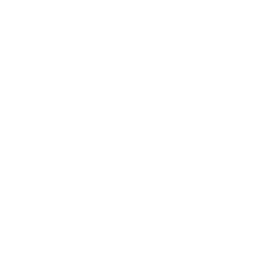
\includegraphics[scale=1]{assets/branding/opa0}
    \vspace{-5.75cm}\\
    {\adjustbox{scale=2.15}{\color{TealDarkCyan}\;IV.\;Cyclic Codes}}
    \bigskip\bigskip
    {\ }\vspace{4cm}\\
    \bigskip
  \end{center}
\end{frame}

%%--- NEW: What Does Cyclic Mean? ---
%\begin{frame}{\textbf{IV. Cyclic Codes}}{What Does ``Cyclic'' Mean?}
%\small
%\begin{columns}[T,onlytextwidth]
%  \begin{column}{.52\textwidth}
%    \textcolor{TealDarkCyan}{\textbf{The core symmetry}}
%
%    A cyclic code is closed under \textbf{rotating} the codeword one position to the right.
%
%    \medskip
%    \begin{center}
%    \begin{tikzpicture}[scale=0.82]
%      % Original codeword
%      \foreach \i/\v in {1/1,2/0,3/1,4/1,5/0,6/1,7/0} {
%        \pgfmathsetmacro{\xp}{(\i-1)*0.72}
%        \node[draw=TealDarkCyan, fill=TealDarkCyan!15, rounded corners=3pt,
%              minimum size=0.65cm, font=\small] at (\xp,0.5) {$\v$};
%      }
%      \node[left=4pt, font=\small, TealDarkCyan] at (-0.1,0.5) {$c=$};
%      % Arrow showing rotation
%      \draw[-Stealth, AccentCyan, thick] (4.5,0.3) -- (4.5,-0.05)
%        node[right=2pt,font=\scriptsize]{rotate};
%      % Rotated codeword
%      \foreach \i/\v in {1/0,2/1,3/0,4/1,5/1,6/0,7/1} {
%        \pgfmathsetmacro{\xp}{(\i-1)*0.72}
%        \node[draw=AccentCyan, fill=AccentCyan!15, rounded corners=3pt,
%              minimum size=0.65cm, font=\small] at (\xp,-0.5) {$\v$};
%      }
%      \node[left=4pt, font=\small, AccentCyan] at (-0.1,-0.5) {$c'=$};
%    \end{tikzpicture}
%    \end{center}
%
%    \medskip
%    If $c = (c_0, c_1, \ldots, c_{n-1})$ is a codeword, so is
%    \[
%      c' = (c_{n-1}, c_0, c_1, \ldots, c_{n-2}).
%    \]
%    Applying the shift repeatedly generates all cyclic shifts of $c$ — and all must be in the code.
%  \end{column}
%  \begin{column}{.45\textwidth}
%    \textcolor{TealDarkCyan}{\textbf{Why is this useful?}}
%    \begin{itemize}
%      \item Shift $=$ multiply by $X$ in the polynomial ring
%      \item Stability under shifts $=$ ideal in $R_n$
%      \item Ideals are generated by a single \emph{generator polynomial} $g(X)$
%      \item Encoding $=$ multiply by $g(X)$ — a simple operation
%    \end{itemize}
%
%    \bigskip
%    \defbox[Hardware bonus]{
%    Cyclic codes can be encoded and decoded with \textbf{shift registers} — fast, cheap circuits. This is why they dominate in hardware applications (CRC, CD, satellite).
%    }
%  \end{column}
%\end{columns}
%\end{frame}

\begin{frame}{\textbf{IV. Cyclic Codes}}{Cyclic shift}
\small
\defbox[Cyclic code]{
A linear code $\code\le\F_q^n$ is cyclic if
\[
  (c_0,c_1,\ldots,c_{n-1})\in\code
  \quad\Rightarrow\quad
  (c_{n-1},c_0,\ldots,c_{n-2})\in\code.
\]
}
\begin{itemize}
  \item This is invariance under a single permutation.
  \item Since the permutation has order $n$, cyclic codes are modules over a cyclic group algebra.
  \item The polynomial model makes this precise.
\end{itemize}
\end{frame}

\begin{frame}{\textbf{IV. Cyclic Codes}}{Polynomial dictionary}
\small
\defbox[Vector to polynomial]{
Identify
\[
  (c_0,c_1,\ldots,c_{n-1})
  \quad\longleftrightarrow\quad
  c(X)=c_0+c_1X+\cdots+c_{n-1}X^{n-1}.
\]
}
\begin{itemize}
  \item Multiplication by $X$ shifts coefficients.
  \item The relation $X^n=1$ performs wrap-around.
  \item Therefore we work modulo $X^n-1$.
\end{itemize}
\end{frame}

\begin{frame}{\textbf{IV. Cyclic Codes}}{The quotient ring}
\small
\defbox[Ambient ring]{
\[
  R_n=\F_q[X]/(X^n-1).
\]
}
\begin{itemize}
  \item Vectors of length $n$ are polynomials of degree $<n$.
  \item Cyclic shift is multiplication by $X$ in $R_n$.
  \item A cyclic code is an $\F_q$-subspace stable under multiplication by $X$.
\end{itemize}
%\begin{block}{Key question}
Which subspaces of $R_n$ are stable under multiplication by $X$?
%\end{block}
\end{frame}

%--- NEW: R_n as a Rotation Carousel ---
\begin{frame}{\textbf{IV. Cyclic Codes}}{$R_n$: The Ring as a Rotation}
\small
\begin{columns}[T,onlytextwidth]
  \begin{column}{.46\textwidth}
    Think of $R_n = \F_q[X]/(X^n-1)$ like a \textbf{clock with $n$ positions} $0,1,\ldots,n-1$.

    \medskip
    Multiplying by $X$ = \textbf{rotating one step}.

    \medskip
    \begin{center}
    \begin{tikzpicture}[scale=1.0]
      % Draw a heptagon (n=7 clock)
      \def\R{1.45}
      \foreach \i in {0,...,6} {
        \pgfmathsetmacro{\ang}{90 - \i*360/7}
        \pgfmathsetmacro{\px}{\R*cos(\ang)}
        \pgfmathsetmacro{\py}{\R*sin(\ang)}
        \fill[TealDarkCyan] (\px,\py) circle (2.8pt);
        \node[font=\tiny\bfseries, TealDarkCyan,
              xshift={0.28cm*cos(\ang)}, yshift={0.28cm*sin(\ang)}]
          at (\px,\py) {$X^{\i}$};
      }
      % Draw the clock circle
      \draw[TealDarkCyan!40, thick] (0,0) circle (\R);
      % Rotation arrow (curved, at top)
      \draw[-Stealth, AccentCyan, thick, bend left=30]
        ({(\R+0.12)*cos(90)},{(\R+0.12)*sin(90)})
        to node[above=2pt,font=\tiny]{$\times X$}
        ({(\R+0.12)*cos(90-360/7)},{(\R+0.12)*sin(90-360/7)});
      % X^7=1 label
      \node[font=\scriptsize, TealDarkCyan] at (0,-0.1) {$X^7=1$};
    \end{tikzpicture}
    \end{center}
  \end{column}
  \begin{column}{.51\textwidth}
    \textcolor{TealDarkCyan}{\textbf{From integers to polynomials}}

    \begin{center}
    \begin{tabular}{c|c}
      $\Z/n\Z$ & $\F_q[X]/(X^n{-}1)$ \\\hline
      \rowcolor{TealDarkCyan!8}
      add $n$ to get $0$ & $X^n = 1$ \\
      $+1$ = shift right & $\times X$ = shift \\
      \rowcolor{TealDarkCyan!8}
      subgroup = ideal & subspace closed\\
                       & under $\times X$ = ideal\\
    \end{tabular}
    \end{center}

    \medskip
    \defbox[Why this matters]{
    A cyclic code is a subspace of $R_n$ that is \emph{closed under rotation}. That is exactly an \textbf{ideal} — generated by a single divisor $g(X)$ of $X^n-1$.
    }
  \end{column}
\end{columns}
\end{frame}

\begin{frame}{\textbf{IV. Cyclic Codes}}{Ideals}
\small
\thmbox[Cyclic codes are ideals]{
Under the identification $\F_q^n\cong R_n$, cyclic codes are exactly the ideals of $R_n$.
}
%\begin{proof}
%If $\code$ is stable under multiplication by $X$, then it is stable under multiplication by every polynomial in $X$. Hence it is an ideal. The converse is immediate.
%\end{proof}
%\begin{block}{Consequence}
%The classification of cyclic codes is an ideal-theoretic problem.
%\end{block}
\end{frame}

\begin{frame}{\textbf{IV. Cyclic Codes}}{Principal ideals}
\small
\thmbox[Principal generator]{
Every ideal of $R_n$ is generated by a unique monic divisor $g(X)$ of $X^n-1$:
\[
  \code=(g(X)).
\]
}
\begin{itemize}
  \item This follows from the principal ideal property of $\F_q[X]$.
  \item The generator polynomial is the monic element of least degree in the code.
  \item The divisibility condition is $g(X)\mid X^n-1$.
\end{itemize}
\end{frame}

\begin{frame}{\textbf{IV. Cyclic Codes}}{Dimension}
\small
\thmbox[Dimension formula]{
If $\code=(g(X))\subseteq R_n$ and $\deg g=r$, then
\[
  \dim_{\F_q}\code=n-r.
\]
}
%\begin{proof}
%The polynomials
%\[
%  g(X),Xg(X),\ldots,X^{n-r-1}g(X)
%\]
%form an $\F_q$-basis of the ideal.
%\end{proof}
\end{frame}

\begin{frame}{\textbf{IV. Cyclic Codes}}{Generator matrix from shifts}
\small
If
\[
  g(X)=g_0+g_1X+\cdots+g_rX^r,
\]
then a generator matrix is obtained by shifting the coefficient vector:
\[
\begin{bmatrix}
g_0&g_1&\cdots&g_r&0&\cdots&0\\
0&g_0&g_1&\cdots&g_r&\cdots&0\\
\vdots&&\ddots&&&\ddots&\vdots
\end{bmatrix}.
\]
\begin{itemize}
  \item This matrix is Toeplitz-like.
  \item It encodes multiplication by $g(X)$.
\end{itemize}
\end{frame}

%--- NEW: Circulant / Shifted Structure ---
\begin{frame}{\textbf{IV. Cyclic Codes}}{The Shifted (Toeplitz) Structure of the Generator Matrix}
\small
For $g(X)=X^3+X+1$ and the $[7,4,3]$ cyclic code, the generator matrix is:
\[
G = \begin{bmatrix}
\mathbf{1}&\mathbf{1}&\mathbf{0}&\mathbf{1}&0&0&0\\
0&\mathbf{1}&\mathbf{1}&\mathbf{0}&\mathbf{1}&0&0\\
0&0&\mathbf{1}&\mathbf{1}&\mathbf{0}&\mathbf{1}&0\\
0&0&0&\mathbf{1}&\mathbf{1}&\mathbf{0}&\mathbf{1}
\end{bmatrix}
\]

\begin{center}
\begin{tikzpicture}[scale=0.82]
  % Draw the 4x7 matrix as colored cells
  % Row i, col j (0-indexed). Entry is 1 if the row is a shift of [1,1,0,1,0,0,0]
  % Row 0: [1,1,0,1,0,0,0]
  % Row 1: [0,1,1,0,1,0,0]
  % Row 2: [0,0,1,1,0,1,0]
  % Row 3: [0,0,0,1,1,0,1]
  % Entries that are 1 (from g coefficients):
  % Row 0: cols 0,1,3
  % Row 1: cols 1,2,4
  % Row 2: cols 2,3,5
  % Row 3: cols 3,4,6
  \foreach \row in {0,1,2,3} {
    \foreach \col in {0,...,6} {
      \pgfmathsetmacro{\xp}{0.72*\col}
      \pgfmathsetmacro{\yp}{-0.55*\row}
      % check if this cell is 1 or 0
      % Row r has 1s at cols r, r+1, r+3 (mod 7, but since all <7, no mod needed)
      % col == row, row+1, or row+3 → cell is 1; else 0
      % (\d is LaTeX's dot-below accent, so use \da/\db/\dc as safe names)
      \pgfmathtruncatemacro{\da}{\col-\row}
      \pgfmathtruncatemacro{\db}{\col-\row-1}
      \pgfmathtruncatemacro{\dc}{\col-\row-3}
      \ifnum\da=0
        \node[draw=AccentCyan,fill=AccentCyan!22,rounded corners=2pt,
              minimum size=0.62cm,font=\small\bfseries] at (\xp,\yp) {1};
      \else\ifnum\db=0
        \node[draw=AccentCyan,fill=AccentCyan!22,rounded corners=2pt,
              minimum size=0.62cm,font=\small\bfseries] at (\xp,\yp) {1};
      \else\ifnum\dc=0
        \node[draw=AccentCyan,fill=AccentCyan!22,rounded corners=2pt,
              minimum size=0.62cm,font=\small\bfseries] at (\xp,\yp) {1};
      \else
        \node[draw=TealDarkCyan!30,fill=TealDarkCyan!5,rounded corners=2pt,
              minimum size=0.62cm,font=\small] at (\xp,\yp) {0};
      \fi\fi\fi
    }
  }
  % Diagonal shift arrows
  \draw[-Stealth,AccentCyan,dashed,thick]
    (-0.5,-0.0) -- (-0.5,-0.55)
    node[left,font=\tiny]{shift};
\end{tikzpicture}
\end{center}

\vspace{-4pt}
\begin{itemize}
  \item Each row is a \textbf{one-position cyclic shift} of the row above
  \item The non-zero diagonals follow the pattern of $g$'s coefficients $(1,1,0,1)$
  \item This ``staircase'' pattern is what makes encoding a shift-register operation
\end{itemize}
\end{frame}

\begin{frame}{\textbf{IV. Cyclic Codes}}{Parity-check polynomial}
\small
\defbox[Check polynomial]{
If $g(X)\mid X^n-1$, define
\[
  h(X)=\frac{X^n-1}{g(X)}.
\]
}
\begin{itemize}
  \item $\deg h=k$ when $\code$ has dimension $k$.
  \item Since $g(X)h(X)=0$ in $R_n$, multiplication by $h(X)$ checks membership.
  \item More precisely, $c(X)\in(g)$ implies $c(X)h(X)\equiv0\pmod{X^n-1}$.
\end{itemize}
\end{frame}

\begin{frame}{\textbf{IV. Cyclic Codes}}{Reciprocal polynomials}
\small
\defbox[Reciprocal]{
For $f(X)=f_0+\cdots+f_mX^m$ with $f_0\ne0$, define
\[
  f^*(X)=X^mf(X^{-1}).
\]
}
\begin{itemize}
  \item Parity-check matrices are naturally written using reciprocal polynomials.
  \item The dual of a cyclic code is cyclic.
  \item If $\code=(g)$ and $h=(X^n-1)/g$, then $\code^\perp$ is generated by a reciprocal of $h$.
\end{itemize}
\end{frame}

\begin{frame}{\textbf{IV. Cyclic Codes}}{Idempotents}
\small
\defbox[Idempotent generator]{
When $\gcd(n,q)=1$, each cyclic code has a unique idempotent generator $e(X)$ satisfying
\[
  e(X)^2=e(X),\qquad \code=(e(X)).
\]
}
\begin{itemize}
  \item Idempotents decompose the semisimple ring $R_n$.
  \item They expose the representation-theoretic structure.
  \item Generator polynomials are usually better for computation.
\end{itemize}
\end{frame}

\begin{frame}{\textbf{IV. Cyclic Codes}}{Roots}
\small
Let $\alpha$ be an $n$-th root of unity in an extension field.
\begin{itemize}
  \item A cyclic code generated by $g(X)$ has zeros $\alpha^i$ where $g(\alpha^i)=0$.
  \item The defining set is
  \[
    Z(\code)=\{i\pmod n:g(\alpha^i)=0\}.
  \]
  \item Root sets translate algebraic divisibility into combinatorics modulo $n$.
\end{itemize}
\end{frame}

\begin{frame}{\textbf{IV. Cyclic Codes}}{Cyclotomic cosets}
\small
\defbox[Q-cyclotomic coset]{
Modulo $n$, the $q$-cyclotomic coset of $i$ is
\[
  C_i=\{i,iq,iq^2,\ldots\}\pmod n.
\]
}
\begin{itemize}
  \item If $\alpha^i$ is a root over $\F_q$, all conjugates $\alpha^{iq^j}$ are roots.
  \item Therefore defining sets are unions of cyclotomic cosets.
  \item Minimal polynomials correspond to these cosets.
\end{itemize}
\end{frame}

%--- NEW: Cyclotomic Cosets Visual for n=7 ---
\begin{frame}{\textbf{IV. Cyclic Codes}}{Cyclotomic Cosets for $n=7$, $q=2$: Orbits Under $\times 2$}
\small
\begin{columns}[T,onlytextwidth]
  \begin{column}{.50\textwidth}
    Multiplying by $q=2$ modulo $n=7$ partitions $\{0,1,\ldots,6\}$ into orbits:

    \medskip
    \begin{center}
    \begin{tikzpicture}[scale=1.0]
      \def\R{1.5}
      % Draw circle
      \draw[TealDarkCyan!30,thick] (0,0) circle (\R);
      % Place 7 points at positions 0..6
      % Position i at angle 90 - i*360/7
      % C_0 = {0}: gray
      \pgfmathsetmacro{\ang}{90}
      \fill[gray!50] ({\R*cos(\ang)},{\R*sin(\ang)}) circle (4pt);
      \node[font=\scriptsize,gray,xshift={0.32cm*cos(\ang)},yshift={0.32cm*sin(\ang)}]
        at ({\R*cos(\ang)},{\R*sin(\ang)}) {$0$};
      % C_1 = {1,2,4}: TealDarkCyan
      \foreach \i in {1,2,4} {
        \pgfmathsetmacro{\ang}{90-\i*360/7}
        \fill[TealDarkCyan] ({\R*cos(\ang)},{\R*sin(\ang)}) circle (4pt);
        \node[font=\scriptsize\bfseries,TealDarkCyan,
              xshift={0.32cm*cos(\ang)},yshift={0.32cm*sin(\ang)}]
          at ({\R*cos(\ang)},{\R*sin(\ang)}) {$\i$};
      }
      % C_3 = {3,5,6}: AccentCyan
      \foreach \i in {3,5,6} {
        \pgfmathsetmacro{\ang}{90-\i*360/7}
        \fill[AccentCyan] ({\R*cos(\ang)},{\R*sin(\ang)}) circle (4pt);
        \node[font=\scriptsize\bfseries,AccentCyan,
              xshift={0.32cm*cos(\ang)},yshift={0.32cm*sin(\ang)}]
          at ({\R*cos(\ang)},{\R*sin(\ang)}) {$\i$};
      }
      % Orbit arrows for C_1: 1->2->4->1
      \pgfmathsetmacro{\aone}{90-1*360/7}
      \pgfmathsetmacro{\atwo}{90-2*360/7}
      \pgfmathsetmacro{\afour}{90-4*360/7}
      \draw[-Stealth,TealDarkCyan,thick,bend left=15]
        ({\R*cos(\aone)},{\R*sin(\aone)}) to ({\R*cos(\atwo)},{\R*sin(\atwo)});
      \draw[-Stealth,TealDarkCyan,thick,bend left=15]
        ({\R*cos(\atwo)},{\R*sin(\atwo)}) to ({\R*cos(\afour)},{\R*sin(\afour)});
      \draw[-Stealth,TealDarkCyan,thick,bend left=15]
        ({\R*cos(\afour)},{\R*sin(\afour)}) to ({\R*cos(\aone)},{\R*sin(\aone)});
      % Orbit arrows for C_3: 3->6->5->3
      \pgfmathsetmacro{\athree}{90-3*360/7}
      \pgfmathsetmacro{\asix}{90-6*360/7}
      \pgfmathsetmacro{\afive}{90-5*360/7}
      \draw[-Stealth,AccentCyan,thick,bend right=15]
        ({\R*cos(\athree)},{\R*sin(\athree)}) to ({\R*cos(\asix)},{\R*sin(\asix)});
      \draw[-Stealth,AccentCyan,thick,bend right=15]
        ({\R*cos(\asix)},{\R*sin(\asix)}) to ({\R*cos(\afive)},{\R*sin(\afive)});
      \draw[-Stealth,AccentCyan,thick,bend right=15]
        ({\R*cos(\afive)},{\R*sin(\afive)}) to ({\R*cos(\athree)},{\R*sin(\athree)});
      % Label ×2
      \node[font=\tiny,TealDarkCyan] at (0.55,0.35) {$\times2$};
      \node[font=\tiny,AccentCyan]   at (-0.55,-0.35) {$\times2$};
    \end{tikzpicture}
    \end{center}
  \end{column}
  \begin{column}{.47\textwidth}
    \textcolor{TealDarkCyan}{\textbf{Three cosets:}}

    \begin{tabular}{c|c|l}
      Coset & Elements & Min. poly \\\hline
      \rowcolor{TealDarkCyan!8}
      $C_0$ & $\{0\}$ & $X+1$ \\
      $C_1$ & $\{1,2,4\}$ & $X^3+X+1$ \\
      \rowcolor{TealDarkCyan!8}
      $C_3$ & $\{3,5,6\}$ & $X^3+X^2+1$ \\
    \end{tabular}

    \medskip
    This gives the factorization:
    \[
      X^7-1 = \underbrace{(X+1)}_{C_0}\underbrace{(X^3+X+1)}_{C_1}\underbrace{(X^3+X^2+1)}_{C_3}
    \]

    \smallskip
    \textbf{Cyclic codes} = choose a subset of factors as the generator $g(X)$.
  \end{column}
\end{columns}
\end{frame}

\begin{frame}{\textbf{IV. Cyclic Codes}}{Minimal polynomials}
\small
\defbox[Minimal polynomial]{
For $\alpha^i$, the minimal polynomial over $\F_q$ is
\[
  M_i(X)=\prod_{j\in C_i}(X-\alpha^j).
\]
}
\begin{itemize}
  \item It lies in $\F_q[X]$.
  \item It is irreducible.
  \item Generator polynomials of cyclic codes are products of such $M_i(X)$.
\end{itemize}
\end{frame}

\begin{frame}{\textbf{IV. Cyclic Codes}}{BCH codes}
\small
\defbox[BCH design]{
A BCH code is a cyclic code whose generator polynomial has a prescribed block of consecutive roots.
}
\[
  g(\alpha^b)=g(\alpha^{b+1})=\cdots=g(\alpha^{b+\delta-2})=0.
\]
\begin{itemize}
  \item The integer $\delta$ is the designed distance.
  \item Consecutive roots force many syndromes to vanish.
  \item The BCH bound converts this into a distance guarantee.
\end{itemize}
\end{frame}

%%--- NEW: BCH Roots on the Circle ---
%\begin{frame}{\textbf{IV. Cyclic Codes}}{BCH Design: Consecutive Roots on the Circle}
%\small
%\begin{columns}[T,onlytextwidth]
%  \begin{column}{.48\textwidth}
%    \textbf{Idea:} place $n$ roots of unity on a circle. Prescribe $\delta-1$ \textcolor{AccentCyan}{\textbf{consecutive}} ones as roots of $g(X)$. The BCH bound guarantees $d \ge \delta$.
%
%    \medskip
%    \begin{center}
%    \begin{tikzpicture}[scale=0.85]
%      % Unit circle
%      \draw[TealDarkCyan!30,thick] (0,0) circle (1.5);
%      % n=7 roots, labeled alpha^0..alpha^6
%      \foreach \i in {0,...,6} {
%        \pgfmathsetmacro{\ang}{90-\i*360/7}
%        \pgfmathsetmacro{\px}{1.5*cos(\ang)}
%        \pgfmathsetmacro{\py}{1.5*sin(\ang)}
%        \ifnum\i=0
%          \fill[gray] (\px,\py) circle (3.2pt);
%          \node[font=\tiny,gray,xshift={0.3cm*cos(\ang)},yshift={0.3cm*sin(\ang)}]
%            at (\px,\py) {$\alpha^0$};
%        \else\ifnum\i=1
%          \fill[AccentCyan] (\px,\py) circle (4pt);
%          \node[font=\tiny\bfseries,AccentCyan,xshift={0.3cm*cos(\ang)},yshift={0.3cm*sin(\ang)}]
%            at (\px,\py) {$\alpha^1$};
%        \else\ifnum\i=2
%          \fill[AccentCyan] (\px,\py) circle (4pt);
%          \node[font=\tiny\bfseries,AccentCyan,xshift={0.3cm*cos(\ang)},yshift={0.3cm*sin(\ang)}]
%            at (\px,\py) {$\alpha^2$};
%        \else
%          \fill[TealDarkCyan!50] (\px,\py) circle (3pt);
%          \node[font=\tiny,TealDarkCyan!70,xshift={0.3cm*cos(\ang)},yshift={0.3cm*sin(\ang)}]
%            at (\px,\py) {$\alpha^{\i}$};
%        \fi\fi\fi
%      }
%      % Arc highlighting the 2 consecutive roots (delta-1=2)
%      \draw[AccentCyan,very thick]
%        ({1.65*cos(90-1*360/7)},{1.65*sin(90-1*360/7)})
%        arc[radius=1.65, start angle={90-1*360/7}, end angle={90-2*360/7}];
%      \node[font=\tiny,AccentCyan] at (1.3,0.8) {$\delta{-}1=2$};
%    \end{tikzpicture}
%    \end{center}
%  \end{column}
%  \begin{column}{.49\textwidth}
%    \textcolor{TealDarkCyan}{\textbf{BCH codes with $n=7$, $q=2$:}}
%
%    \medskip
%    \begin{tabular}{c|l|c|c}
%      $\delta$ & roots of $g$ & $[n,k]$ & $d$ \\\hline
%      \rowcolor{TealDarkCyan!8}
%      3 & $\alpha^1,\alpha^2$ & $[7,4]$ & 3 (Hamming) \\
%      5 & $\alpha^1,\ldots,\alpha^4$ & $[7,1]$ & 7 (repetition) \\
%    \end{tabular}
%
%    \medskip
%    \begin{block}{BCH Bound}
%    $\delta-1$ consecutive roots $\Rightarrow d \ge \delta$. More prescribed roots $\Rightarrow$ higher designed distance $\Rightarrow$ lower rate.
%    \end{block}
%
%    \medskip
%    \textcolor{TealDarkCyan}{\textbf{Key insight for non-majors:}} prescribing more roots forces the codeword polynomial to have more zeros, which ``spreads'' the code and increases the minimum distance — at the cost of fewer codewords (lower rate).
%  \end{column}
%\end{columns}
%\end{frame}

\begin{frame}{\textbf{IV. Cyclic Codes}}{BCH bound}
\small
\thmbox[BCH bound]{
If a cyclic code has $\delta-1$ consecutive roots
\[
  \alpha^b,\alpha^{b+1},\ldots,\alpha^{b+\delta-2},
\]
then its minimum distance is at least $\delta$.
}
%\begin{proof}
%A codeword of weight $<\delta$ would give a nonzero polynomial with too many consecutive zero syndromes, forcing a Vandermonde determinant to vanish.
%\end{proof}
\end{frame}

\begin{frame}{\textbf{IV. Cyclic Codes}}{Narrow-sense primitive BCH}
\small
\defbox[Common special case]{
Let $n=q^m-1$ and let $\alpha$ be primitive in $\F_{q^m}$. The narrow-sense BCH code of designed distance $\delta$ has roots
\[
  \alpha,\alpha^2,\ldots,\alpha^{\delta-1}.
\]
}
\begin{itemize}
  \item Primitive: the length is the full multiplicative order.
  \item Narrow-sense: the first root is $\alpha$.
  \item Hamming codes occur when $\delta=3$ in the binary case.
\end{itemize}
\end{frame}

\begin{frame}{\textbf{IV. Cyclic Codes}}{Cyclic Hamming code}
\small
Let $n=2^r-1$ and let $\alpha\in\F_{2^r}$ be primitive.
\begin{itemize}
  \item Let $g(X)$ be the minimal polynomial of $\alpha$ over $\F_2$.
  \item Then $\deg g=r$.
  \item The cyclic code $(g)$ has parameters
  \[
    [2^r-1,2^r-1-r,3]_2.
  \]
\end{itemize}
%\begin{block}{Identification}
This is the binary Hamming code in cyclic coordinates.
%\end{block}
\end{frame}

\begin{frame}{\textbf{IV. Cyclic Codes}}{The case n equals 7}
\small
Over $\F_2$,
\[
  X^7-1=(X+1)(X^3+X+1)(X^3+X^2+1).
\]
\begin{itemize}
  \item A primitive $7$-th root has minimal polynomial $X^3+X+1$ or $X^3+X^2+1$.
  \item Either cubic gives a cyclic $[7,4,3]$ Hamming code.
  \item The two choices are equivalent under coordinate reversal.
\end{itemize}
\end{frame}

\begin{frame}{\textbf{IV. Cyclic Codes}}{Encoding by multiplication}
\small
For a cyclic code $(g)$ with $\deg g=r$, non-systematic encoding is
\[
  m(X)\longmapsto c(X)=m(X)g(X),\qquad \deg m< n-r.
\]
\begin{itemize}
  \item The message polynomial has $k=n-r$ coefficients.
  \item The product automatically lies in the ideal $(g)$.
  \item Hardware can implement this multiplication by shift registers.
\end{itemize}
\end{frame}

\begin{frame}{\textbf{IV. Cyclic Codes}}{Systematic cyclic encoding}
\small
Let $\deg g=r$. To encode a message $m(X)$ with $\deg m<k$:
\[
  X^r m(X)=q(X)g(X)+p(X),\qquad \deg p<r.
\]
Then set
\[
  c(X)=X^rm(X)-p(X).
\]
\begin{itemize}
  \item Since $c(X)$ is divisible by $g(X)$, it is a codeword.
  \item The high-degree coefficients contain the message.
  \item The low-degree polynomial $p(X)$ supplies parity.
\end{itemize}
\end{frame}

%%--- NEW: Systematic Encoding Walkthrough ---
%\begin{frame}{\textbf{IV. Cyclic Codes}}{Systematic Encoding: Step-by-Step Example}
%\small
%Encode message $m(X) = X^3 + 1$ (i.e.\ $m=(1,0,0,1)$) using $g(X)=X^3+X+1$.
%
%\medskip
%\begin{center}
%\begin{tikzpicture}[scale=0.88,
%  sbox/.style={draw=TealDarkCyan,thick,rounded corners=4pt,
%               fill=TealDarkCyan!8,minimum width=5.2cm,
%               minimum height=0.55cm,font=\scriptsize,align=left}]
%  \node[sbox] at (0,3.4) {\textbf{Step 1.} Form $X^3 m(X) = X^6+X^3$};
%  \node[sbox] at (0,2.75) {\textbf{Step 2.} Divide: $X^6+X^3 = (X^3+X^2+X+1)\cdot g(X) + (X^2+X)$};
%  \node[sbox,fill=AccentCyan!10,draw=AccentCyan] at (0,2.1)
%    {\textbf{Step 3.} Remainder $p(X) = X^2+X$ (the parity part)};
%  \node[sbox] at (0,1.45)
%    {\textbf{Step 4.} Codeword: $c(X)=X^3 m(X)-p(X)=X^6+X^3+X^2+X$};
%  \node[sbox,fill=TealDarkCyan!15] at (0,0.8)
%    {\textbf{Check:} $c(X)\div g(X)=(X^3+X^2+X+1)$ — remainder 0 \checkmark};
%\end{tikzpicture}
%\end{center}
%
%\vspace{-2pt}
%\begin{columns}[T,onlytextwidth]
%  \begin{column}{.50\textwidth}
%    \textbf{Codeword in vector form:}
%    \[
%      c = (0,1,1,1,0,0,1) \in \F_2^7
%    \]
%    \begin{itemize}
%      \item Bits 4--7 (positions $X^3,\ldots,X^6$): the message $(1,0,0,1)$
%      \item Bits 1--3: the parity $(0,1,1)$ from $p(X)=X^2+X$
%    \end{itemize}
%  \end{column}
%  \begin{column}{.47\textwidth}
%%    \begin{block}{Why this works}
%    Since $c(X) = X^3 m(X) - p(X)$ and $p(X) \equiv X^3 m(X) \pmod{g}$, we get $c(X) \equiv 0 \pmod{g}$. So $c$ is a codeword.
%%    \end{block}
%  \end{column}
%\end{columns}
%\end{frame}
%
%\begin{frame}{\textbf{IV. Cyclic Codes}}{Syndrome polynomial}
%\small
%For received $v(X)=c(X)+e(X)$, compute the remainder
%\[
%  s(X)=v(X)\bmod g(X).
%\]
%\begin{itemize}
%  \item Since $c(X)$ is divisible by $g(X)$, $s(X)=e(X)\bmod g(X)$.
%  \item This is the polynomial analogue of $Hv^T=He^T$.
%  \item BCH decoding refines this by evaluating at roots of $g$.
%\end{itemize}
%\end{frame}
%
%\begin{frame}{\textbf{IV. Cyclic Codes}}{Root syndromes}
%\small
%If $\alpha^i$ is a root of $g(X)$, then every codeword satisfies
%\[
%  c(\alpha^i)=0.
%\]
%For $v=c+e$,
%\[
%  v(\alpha^i)=e(\alpha^i).
%\]
%\begin{itemize}
%  \item The numbers $S_i=v(\alpha^i)$ are syndromes.
%  \item Decoding asks for the error locations and values from these sums.
%  \item This is a finite-field moment problem.
%\end{itemize}
%\end{frame}
%
%\begin{frame}{\textbf{IV. Cyclic Codes}}{Error locator polynomial}
%\small
%For error locations $j_1,\ldots,j_t$, define
%\[
%  \Lambda(Z)=\prod_{\ell=1}^t(1-\alpha^{j_\ell}Z).
%\]
%\begin{itemize}
%  \item The roots of $\Lambda$ identify error locations.
%  \item BCH and Reed--Solomon decoding compute $\Lambda$ from syndromes.
%  \item Berlekamp--Massey is an efficient algorithm for this recurrence problem.
%\end{itemize}
%\end{frame}
%
%\begin{frame}{\textbf{IV. Cyclic Codes}}{LFSR viewpoint}
%\small
%\defbox[Linear feedback shift register]{
%Division by $g(X)$ can be implemented with a shift register whose feedback taps are the nonzero coefficients of $g(X)$.
%}
%\begin{itemize}
%  \item Memory cost is $\deg g=n-k$ registers.
%  \item Input is processed one symbol per clock.
%  \item This is why cyclic codes became central in hardware error control.
%\end{itemize}
%\end{frame}
%
%%--- NEW: LFSR Circuit Diagram ---
%\begin{frame}{\textbf{IV. Cyclic Codes}}{The LFSR Circuit for $g(X)=X^3+X+1$}
%\small
%For the $[7,4,3]$ cyclic Hamming code, $g(X)=X^3+X+1$. The feedback taps are at $X^0$ and $X^1$.
%
%\medskip
%\begin{center}
%\begin{tikzpicture}[
%  reg/.style  = {draw=TealDarkCyan, thick, rectangle,
%                 minimum width=0.9cm, minimum height=0.7cm, fill=TealDarkCyan!12},
%  xorcirc/.style = {draw=AccentCyan, thick, circle,
%                    minimum size=0.5cm, fill=AccentCyan!15, font=\small},
%  arr/.style  = {-Stealth, thick, TealDarkCyan},
%  farr/.style = {-Stealth, thick, AccentCyan, dashed}
%]
%  % Input node
%  \node[font=\small] (inp) at (-2.5,0) {input $b_i$};
%  % XOR gates
%  \node[xorcirc] (x1) at (-1.2,0) {$\oplus$};
%  \node[xorcirc] (x2) at ( 1.4,0) {$\oplus$};
%  % Registers R0, R1, R2
%  \node[reg] (R0) at (0,   0) {$R_0$};
%  \node[reg] (R1) at (2.6, 0) {$R_1$};
%  \node[reg] (R2) at (4.6, 0) {$R_2$};
%  % Forward connections
%  \draw[arr] (inp) -- (x1);
%  \draw[arr] (x1)  -- (R0);
%  \draw[arr] (R0)  -- (x2);
%  \draw[arr] (x2)  -- (R1);
%  \draw[arr] (R1)  -- (R2);
%  \node[right=4pt,font=\small] at (R2.east) {$\to$ parity out};
%  % Feedback from R2 back to x1 (tap for $g_0=1$, i.e.\ $X^0$)
%  \draw[farr] (R2.south) -- ++(0,-0.55) -| (x1.south)
%    node[near start, below, font=\tiny, AccentCyan]{tap $X^0$};
%  % Feedback from R2 back to x2 (tap for $g_1=1$, i.e.\ $X^1$)
%  \draw[farr] (R2.south)++(0,-0.55) -- ++(0,0) -| (x2.south)
%    node[near end, below, font=\tiny, AccentCyan]{tap $X^1$};
%  % Label
%  \node[font=\scriptsize, TealDarkCyan] at (1.15,-1.4)
%    {Computes remainder of $X^3 \cdot m(X) \div g(X)$ — one bit per clock};
%\end{tikzpicture}
%\end{center}
%
%\begin{columns}[T,onlytextwidth]
%  \begin{column}{.48\textwidth}
%    \textbf{Encoding (4 clock cycles):}
%    \begin{enumerate}\small
%      \item Feed in the $4$ message bits $m_3,m_2,m_1,m_0$
%      \item The 3 registers accumulate the parity
%      \item Read off $(R_0, R_1, R_2)$ — these are the 3 parity bits
%    \end{enumerate}
%  \end{column}
%  \begin{column}{.48\textwidth}
%    \textbf{Key advantage:}
%    \begin{itemize}\small
%      \item Only $r = n{-}k$ flip-flops needed
%      \item One XOR gate per feedback tap
%      \item Works at wire speed — no computation delay
%      \item Used in every USB, Ethernet, and SATA controller
%    \end{itemize}
%  \end{column}
%\end{columns}
%\end{frame}
%
%\begin{frame}{\textbf{IV. Cyclic Codes}}{Burst errors}
%\small
%\defbox[Burst]{
%A burst of length $\ell$ is an error whose nonzero positions lie in $\ell$ consecutive coordinates.
%}
%\begin{itemize}
%  \item Polynomial remainders are well suited for burst detection.
%  \item CRC polynomials are chosen to detect common burst patterns.
%  \item This is detection rather than correction in many communication protocols.
%\end{itemize}
%\end{frame}
%
%\begin{frame}{\textbf{IV. Cyclic Codes}}{CRC codes}
%\small
%CRC uses a generator polynomial $g(X)$ and transmits a multiple of $g(X)$.
%\begin{itemize}
%  \item Receiver divides by $g(X)$.
%  \item Nonzero remainder means an error was detected.
%  \item The method is a cyclic-code membership test.
%\end{itemize}
%\begin{block}{Mathematical core}
%CRC is not a different theory: it is cyclic codes used primarily for error detection.
%\end{block}
%\end{frame}
%
%%--- NEW: CRC in Daily Life ---
%\begin{frame}{\textbf{IV. Cyclic Codes}}{CRC in Your Daily Life}
%\small
%\begin{columns}[T,onlytextwidth]
%  \begin{column}{.52\textwidth}
%    \textcolor{TealDarkCyan}{\textbf{Every data transfer uses CRC.}}
%
%    \medskip
%    \begin{tabular}{p{2.3cm}|p{1.4cm}|p{1.5cm}}
%      \textbf{Standard} & \textbf{Polynomial} & \textbf{Detects} \\\hline
%      \rowcolor{TealDarkCyan!8}
%      Ethernet (CRC-32) & $x^{32}+\cdots$ & $\le 32$-bit bursts \\
%      USB 2.0 & CRC-16 & $\le 16$-bit bursts \\
%      \rowcolor{TealDarkCyan!8}
%      SATA/NVMe & CRC-32 & storage errors \\
%      PNG / ZIP & CRC-32 & file corruption \\
%      \rowcolor{TealDarkCyan!8}
%      Bluetooth & CRC-24 & packet errors \\
%    \end{tabular}
%
%    \medskip
%    \textcolor{TealDarkCyan}{\textbf{How it works (in one sentence):}}
%    \begin{itemize}
%      \item Sender appends $r = \deg g$ bits so the extended packet is divisible by $g(X)$
%      \item Receiver divides: nonzero remainder $\Rightarrow$ error detected
%    \end{itemize}
%  \end{column}
%  \begin{column}{.45\textwidth}
%    \begin{tikzpicture}[scale=0.82]
%      % Ethernet frame schematic
%      \node[font=\scriptsize\bfseries, TealDarkCyan] at (1.6,4.0)
%        {Ethernet frame};
%      \node[draw=TealDarkCyan, fill=TealDarkCyan!10, rounded corners=3pt,
%            minimum width=3.2cm, minimum height=0.42cm, font=\tiny]
%        at (1.6,3.55) {Destination MAC (6 B)};
%      \node[draw=TealDarkCyan, fill=TealDarkCyan!10, rounded corners=3pt,
%            minimum width=3.2cm, minimum height=0.42cm, font=\tiny]
%        at (1.6,3.08) {Source MAC (6 B)};
%      \node[draw=TealDarkCyan, fill=TealDarkCyan!10, rounded corners=3pt,
%            minimum width=3.2cm, minimum height=0.42cm, font=\tiny]
%        at (1.6,2.61) {EtherType (2 B)};
%      \node[draw=TealDarkCyan, fill=TealDarkCyan!15, rounded corners=3pt,
%            minimum width=3.2cm, minimum height=0.70cm, font=\tiny]
%        at (1.6,2.00) {Payload (46–1500 B)};
%      \node[draw=AccentCyan, thick, fill=AccentCyan!20, rounded corners=3pt,
%            minimum width=3.2cm, minimum height=0.42cm, font=\tiny\bfseries]
%        at (1.6,1.48) {CRC-32 checksum (4 B)};
%      % Arrow
%      \draw[-Stealth, AccentCyan, thick] (3.3,1.48) -- (4.1,1.48)
%        node[right,font=\tiny]{verify};
%    \end{tikzpicture}
%
%    \smallskip
%    \begin{block}{}
%    \centering\footnotesize
%    CRC detects $\approx 99.9998\%$ of\\ random errors. It does \emph{not} correct them — for correction, add an outer code (e.g.\ Reed--Solomon).
%    \end{block}
%  \end{column}
%\end{columns}
%\end{frame}
%
%%--- NEW: Reed-Solomon Intuition ---
%\begin{frame}{\textbf{IV. Cyclic Codes}}{Reed--Solomon: The Core Idea}
%\small
%\begin{columns}[T,onlytextwidth]
%  \begin{column}{.50\textwidth}
%    \textcolor{TealDarkCyan}{\textbf{The polynomial evaluation idea}}
%
%    \medskip
%    A degree-$(k{-}1)$ polynomial over $\F_q$ is determined by $k$ of its values. If you evaluate it at $n > k$ points and some values are corrupted, you can still recover the polynomial — because \emph{any $k$ correct values suffice}.
%
%    \medskip
%    \begin{center}
%    \begin{tikzpicture}[scale=0.82]
%      \draw[-Stealth, TealDarkCyan, thick] (-0.2,0) -- (3.5,0)
%        node[right, font=\scriptsize]{$\alpha^i$};
%      \draw[-Stealth, TealDarkCyan, thick] (0,-0.2) -- (0,2.4)
%        node[above, font=\scriptsize]{$f(\alpha^i)$};
%      % True polynomial (quadratic)
%      \draw[TealDarkCyan, thick, domain=0.1:3.2, samples=30]
%        plot (\x, {0.4*(\x-1.6)^2+0.5});
%      % Evaluation points
%      \fill[TealDarkCyan] (0.5,{0.4*(0.5-1.6)^2+0.5}) circle (3pt)
%        node[above=2pt,font=\tiny]{ok};
%      \fill[TealDarkCyan] (1.2,{0.4*(1.2-1.6)^2+0.5}) circle (3pt)
%        node[above=2pt,font=\tiny]{ok};
%      \fill[TealDarkCyan] (1.6,0.5) circle (3pt)
%        node[above=2pt,font=\tiny]{ok};
%      \fill[TealDarkCyan] (2.2,{0.4*(2.2-1.6)^2+0.5}) circle (3pt)
%        node[above=2pt,font=\tiny]{ok};
%      % Corrupted points
%      \fill[AccentCyan] (0.9,1.8) circle (3pt)
%        node[right=2pt,font=\tiny,AccentCyan]{err};
%      \fill[AccentCyan] (2.8,0.2) circle (3pt)
%        node[right=2pt,font=\tiny,AccentCyan]{err};
%    \end{tikzpicture}
%    \end{center}
%  \end{column}
%  \begin{column}{.47\textwidth}
%    \defbox[Reed--Solomon $\mathrm{RS}(n,k)$]{
%    \begin{itemize}
%      \item Message: polynomial $f$ of degree $<k$
%      \item Codeword: $(f(\alpha^0),\ldots,f(\alpha^{n-1}))$
%      \item Minimum distance: $d = n-k+1$ (\textbf{MDS})
%      \item Corrects up to $\lfloor(n-k)/2\rfloor$ errors
%    \end{itemize}
%    }
%
%    \bigskip
%    \textcolor{TealDarkCyan}{\textbf{In practice:}}
%    \begin{itemize}
%      \item CD, DVD, Blu-ray: RS$(255,251)$ per 8-bit symbol
%      \item QR codes: up to RS$(255,223)$
%      \item Deep space (Voyager): RS$(255,223)$, corrects up to 16 symbol errors
%    \end{itemize}
%  \end{column}
%\end{columns}
%\end{frame}
%
%\begin{frame}{\textbf{IV. Cyclic Codes}}{Reed--Solomon codes}
%\small
%\defbox[Reed--Solomon]{
%Over $\F_q$, Reed--Solomon codes evaluate polynomials of degree $<k$ at $n$ distinct field points.
%}
%\begin{itemize}
%  \item In a suitable form, they are cyclic codes.
%  \item They meet the Singleton bound: $d=n-k+1$.
%  \item They correct symbol errors, which is why they are strong against bursts.
%\end{itemize}
%\end{frame}
%
%\begin{frame}{\textbf{IV. Cyclic Codes}}{BCH versus Reed--Solomon}
%\small
%\begin{columns}[T,onlytextwidth]
%  \begin{column}{.48\textwidth}
%    \defbox[BCH]{
%    \begin{itemize}\small
%      \item often binary
%      \item roots in an extension field
%      \item designed distance
%      \item strong for bit errors
%    \end{itemize}
%    }
%  \end{column}
%  \begin{column}{.48\textwidth}
%    \defbox[Reed--Solomon]{
%    \begin{itemize}\small
%      \item nonbinary
%      \item evaluation over $\F_q$
%      \item MDS property
%      \item strong for symbol bursts
%    \end{itemize}
%    }
%  \end{column}
%\end{columns}
%\end{frame}
%
%\begin{frame}{\textbf{IV. Cyclic Codes}}{Dual cyclic codes}
%\small
%\thmbox[Dual cyclicity]{
%The dual of a cyclic code is cyclic.
%}
%\begin{proof}
%If $c$ is orthogonal to every word of $\code$, then a cyclic shift of $c$ is also orthogonal to every cyclic shift of every word of $\code$. Since $\code$ is shift-invariant, the shifted $c$ lies in $\code^\perp$.
%\end{proof}
%\begin{itemize}
%  \item Generator polynomials of duals are expressed using reciprocal polynomials.
%  \item This is another sign that cyclic codes form a closed algebraic world.
%\end{itemize}
%\end{frame}
%
%\begin{frame}{\textbf{IV. Cyclic Codes}}{Repeated-root caution}
%\small
%\begin{block}{Assumption often made}
%Many clean statements assume $\gcd(n,q)=1$.
%\end{block}
%\begin{itemize}
%  \item Then $X^n-1$ has no repeated roots.
%  \item The quotient ring is semisimple.
%  \item If $\gcd(n,q)\ne1$, repeated-root cyclic codes require extra care.
%\end{itemize}
%\begin{block}{Moral}
%Always check separability before using root-set arguments naively.
%\end{block}
%\end{frame}
%
%\begin{frame}{\textbf{IV. Cyclic Codes}}{Quasi-cyclic hint}
%\small
%\defbox[Quasi-cyclic code]{
%A code is quasi-cyclic of index $\ell$ if it is invariant under cyclic shift by $\ell$ positions.
%}
%\begin{itemize}
%  \item Generator matrices are built from circulant blocks.
%  \item Circulant blocks correspond to polynomials modulo $X^m-1$.
%  \item This structure is important in code-based cryptography.
%\end{itemize}
%\end{frame}
%
%\begin{frame}{\textbf{IV. Cyclic Codes}}{Algebraic hierarchy}
%\small
%\[
%\begin{array}{c}
%\text{linear code}\\
%\Downarrow\ \text{add cyclic shift}\\
%\text{cyclic code}\\
%\Downarrow\ \text{prescribe roots}\\
%\text{BCH code}\\
%\Downarrow\ \text{evaluation/MDS structure}\\
%\text{Reed--Solomon code}
%\end{array}
%\]
%\begin{block}{Perspective}
%Each additional algebraic structure buys stronger theorems and faster algorithms.
%\end{block}
%\end{frame}
%
%\begin{frame}{\textbf{IV. Cyclic Codes}}{Cyclic codes as modules}
%\small
%\begin{itemize}
%  \item A linear code is an $\F_q$-subspace of $\F_q^n$.
%  \item A cyclic code is an $\F_q[X]$-submodule, where $X$ acts by shift.
%  \item The relation $X^n=1$ makes the module a module over $R_n$.
%\end{itemize}
%\[
%  \text{cyclic code}=\text{submodule of }R_n=\text{ideal of }R_n.
%\]
%\begin{block}{Mathematician's slogan}
%Shift-invariant linear algebra is ideal theory.
%\end{block}
%\end{frame}
%
%\begin{frame}{\textbf{IV. Cyclic Codes}}{Exercise: ideal proof}
%\small
%\begin{block}{Problem}
%Prove that if an $\F_q$-subspace $\code\subseteq R_n$ is closed under multiplication by $X$, then it is an ideal.
%\end{block}
%\textbf{Hint.}
%\begin{itemize}
%  \item Closure under $X$ gives closure under $X^j$ for every $j\ge0$.
%  \item By linearity, closure under every polynomial follows.
%  \item Reduce modulo $X^n-1$.
%\end{itemize}
%\end{frame}
%
%\begin{frame}{\textbf{IV. Cyclic Codes}}{Exercise: dimension}
%\small
%\begin{block}{Problem}
%Let $g(X)\mid X^n-1$ and $\deg g=r$. Show that $(g)$ has dimension $n-r$ as an $\F_q$-space.
%\end{block}
%\textbf{Hint.}
%\[
%  a(X)g(X),\qquad \deg a<n-r
%\]
%are all distinct modulo $X^n-1$.
%\begin{itemize}
%  \item Count the possible coefficients of $a(X)$.
%  \item Use the degree bound to prove injectivity.
%\end{itemize}
%\end{frame}
%
%\begin{frame}{\textbf{IV. Cyclic Codes}}{Exercise: cyclic Hamming}
%\small
%\begin{block}{Problem}
%For $X^7-1=(X+1)(X^3+X+1)(X^3+X^2+1)$ over $\F_2$, show that the code generated by $g=X^3+X+1$ has parameters $[7,4,3]$.
%\end{block}
%\textbf{Hint.}
%\begin{itemize}
%  \item Dimension is $7-\deg g=4$.
%  \item The BCH bound with roots $\alpha,\alpha^2$ gives $d\ge3$.
%  \item The Singleton bound excludes $d>4$, and a direct word gives $d=3$.
%\end{itemize}
%\end{frame}
%
%\begin{frame}{\textbf{IV. Cyclic Codes}}{Summary of cyclic codes}
%\small
%\begin{columns}[T,onlytextwidth]
%  \begin{column}{.48\textwidth}
%    \defbox[Algebra]{
%    \begin{itemize}\small
%      \item $R_n=\F_q[X]/(X^n-1)$
%      \item cyclic codes are ideals
%      \item generator polynomial $g$
%      \item root sets and cosets
%    \end{itemize}
%    }
%  \end{column}
%  \begin{column}{.48\textwidth}
%    \defbox[Algorithms]{
%    \begin{itemize}\small
%      \item encoding by multiplication
%      \item parity by remainders
%      \item BCH decoding from syndromes
%      \item LFSR implementation
%    \end{itemize}
%    }
%  \end{column}
%\end{columns}
%\end{frame}
%
%\begin{frame}{\textbf{IV. Cyclic Codes}}{Final perspective}
%\small
%\begin{alertblock}{}
%\centering
%Linear codes turn error correction into finite-dimensional algebra.\\[4pt]
%Hamming codes show how perfect decoding is finite geometry.\\[4pt]
%Cyclic codes show how shift symmetry becomes polynomial ideal theory.
%\end{alertblock}
%\bigskip
%\begin{center}
%\large
%\textbf{Coding theory is the art of adding structure to redundancy.}
%\end{center}
%\end{frame}


%-------------------------------------------------------
% CLOSING FRAME
%-------------------------------------------------------
\begin{frame}[plain]
  \begin{center}\bfseries\centering
    \vspace{2cm}
    {\Huge\color{TealDarkCyan} Thank You}\\[.5cm]
    {\large\color{black} Ji, Yong-hyeon}\\[.3cm]
    {\normalsize\texttt{hacker3740@gmail.com}}\\[.5cm]
    {\small\color{gray} 2026 Spring $\cdot$ Colloquium $\cdot$ 2026}
    \bigskip
  \end{center}
\end{frame}

\end{document}
